 %-*- TeX:UTF-8:Soft -*-

\textcolor{blue}{MOVE TO PAGE 37 FOR PEAK PRICES RESULTS}

\textcolor{blue}{MOVE TO PAGES 13 AND 16 FOR LEFT DIGITS RESULTS SPLITTING THE SAMPLE BASED ON ANNUAL VOLATILITY}


\section{Left Most Digit}\label{sec:intro}

	Here, we look at what happen when the second left digit moves from 9 to 0 (i.e., when the left most digit changes).
	
Sample restrictions:

\begin{itemize}
	\item New accounts (same sample used in the Disposition Effect Paper for convenience)
	\item The unit of observation is an investor $\times$ stock $\times$ day. 
	\item Sample 1: We use login days and all quarters and stocks in which (1) the price has increased with respect to the initial price of the stock in that quarter and (2) there was at least one change in the first left digit of the price---on any day in the quarter. We use all days in the quarter.
	
	\item For (1), I look at the first price observed by the trader in the quarter and all the prices in the login days during that quarter.
	\item By using (1) and (2) restrictions, we are excluding the quarters in which the stocks have not increase enough to move up the left most digit or have a general tendency to decline.
	
	\item Sample 2: All remaining quarters that were excluded above.
	
	
\end{itemize}	

	


First, I am pooling all the observation to show patterns. But the second digit have bins of different size. As a robustness check, I also have created three subsets to have the same bins on each second digit. These include prices in the intervals £0.11 to £1.01, £1.1 to £10.1, and £11 to £101. In these subsets I only selected the days when the price of the stock was in any of these intervals.



\textcolor{blue}{Why this restrictions? When prices increase during the quarter, the probability to sell moves up when the second digit becomes 0. But the opposite occurs when the prices move down. So the average effect of a change in the left most digit if we pool all the data is cancelled out because we are not distinguishing increments and reductions in prices.}


	
First, I will show the distribution of prices on login days for all the data. Then, some stats for the subsamples.	
	
	\clearpage
	\subsection{Summary Stats}
	
	\begin{figure}%
		\centering%
		\caption{Histogram of Prices, Login-Day Sample}%
		\label{fig:disposition_interaction_main}%
		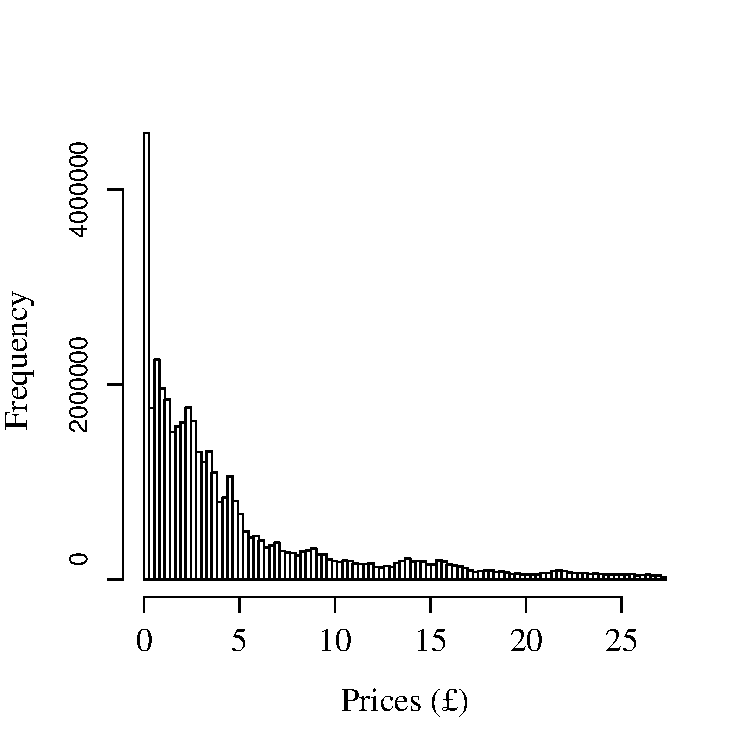
\includegraphics[width=.7\textwidth]{figures/prices_hist_login_days.pdf}
		\fignote{Figure shows the histogram of prices on login days. Outliers in the 99 percentile are excluded.}
	\end{figure}




\clearpage


\begin{econtable}\small
	\caption{Summary Stats}
	\label{tab:stats}
	\estauto{lcccccccc}{
	& \multicolumn{1}{c}{N} & \multicolumn{1}{c}{Mean} & \multicolumn{1}{c}{St. Dev.} & \multicolumn{1}{c}{Min} & \multicolumn{1}{c}{Pctl(25)} & \multicolumn{1}{c}{Median} & \multicolumn{1}{c}{Pctl(75)} & \multicolumn{1}{c}{Max} \\ 	
		Price on Login Days \pounds & 43,903,112 & 7.942 & 26.178 & 0.000 & 1.153 & 3.050 & 7.642 & 15,051.630 \\ 
Price on Sell Days \pounds & 3,341,054 & 7.103 & 24.523 & 0.000 & 0.832 & 2.646 & 6.674 & 3,589.000 \\ 
Price of Stocks Sold \pounds & 342,277 & 6.848 & 16.483 & 0.000 & 0.861 & 2.714 & 6.648 & 1,771.425 \\ 
 
	}
	\fignote{Sample of all investor $\times$ stock $\times$ days on which the investor log in to his account. }
\end{econtable}





\begin{econtable}[h]\small
	\caption{Summary Stats for Subsamples  - Quarters when Stocks Increased in Price}
	\label{tab:stats}
	\estauto{lcccccccc}{
		& \multicolumn{1}{c}{N} & \multicolumn{1}{c}{Mean} & \multicolumn{1}{c}{St. Dev.} & \multicolumn{1}{c}{Min} & \multicolumn{1}{c}{Pctl(25)} & \multicolumn{1}{c}{Median} & \multicolumn{1}{c}{Pctl(75)} & \multicolumn{1}{c}{Max} \\ 	
		All Stocks & 316,242 & 5.777 & 15.384 & 0.000 & 0.582 & 2.433 & 6.010 & 2,001.557 \\ 
Stocks with Prices Between \pounds 0.11 to \pounds 1.01 & 82,932 & 0.588 & 0.254 & 0.110 & 0.378 & 0.616 & 0.795 & 1.010 \\ 
Stocks with Prices Between \pounds 1.1 to \pounds 10.1 & 155,842 & 4.816 & 2.367 & 1.100 & 2.917 & 4.348 & 6.578 & 10.099 \\ 
Stocks with Prices Between \pounds 11 to \pounds 101 & 25,401 & 34.166 & 18.423 & 11.000 & 19.931 & 30.040 & 46.290 & 100.690 \\ 
 
	}
	\fignote{The unit of observation is an investor $\times$ stock $\times$ day. The samples is restricted to login days. We include only quarters in which the stocks increased in price (regarding the first observation of the quarter) and change the left most digit at least once during the quarter. Only those stocks that have changed the left most digit are included.}
\end{econtable}


\begin{econtable}[h]\small
	\caption{Summary Stats for Subsamples - Remaining Quarters}
	\label{tab:stats}
	\estauto{lcccccccc}{
		& \multicolumn{1}{c}{N} & \multicolumn{1}{c}{Mean} & \multicolumn{1}{c}{St. Dev.} & \multicolumn{1}{c}{Min} & \multicolumn{1}{c}{Pctl(25)} & \multicolumn{1}{c}{Median} & \multicolumn{1}{c}{Pctl(75)} & \multicolumn{1}{c}{Max} \\ 	
		All Stocks & 4,376,352 & 7.507 & 26.412 & 0.000 & 1.183 & 2.650 & 8.270 & 4,495.251 \\ 
Stocks with Prices Between \pounds 0.10 to \pounds 1.0 & 611,813 & 0.491 & 0.277 & 0.100 & 0.226 & 0.472 & 0.740 & 1.000 \\ 
Stocks with Prices Between \pounds 1 to \pounds 10 & 2,461,228 & 3.230 & 1.998 & 1.000 & 1.750 & 2.602 & 4.176 & 10.000 \\ 
Stocks with Prices Between \pounds 10 to \pounds 100 & 978,415 & 20.993 & 11.905 & 10.000 & 13.725 & 16.350 & 24.450 & 99.990 \\ 
 
	}
	\fignote{The unit of observation is an investor $\times$ stock $\times$ day. The samples is restricted to login days. We include the remaining quarters in which the stocks did not increase their prices and change the left most digit at least once during the quarter.}
\end{econtable}


\clearpage

\subsection{Effect of Left Digits When Prices Increase}

\subsubsection{Raw Patterns Showing the First Two Digits and the Probability to Sell}


\begin{figure}[hbt!]
	\centering%
	\caption{Probability of Selling  for Stocks that Change the First Digit \\ All Stocks (different bin size)}%
	\label{fig:all_obs}%
	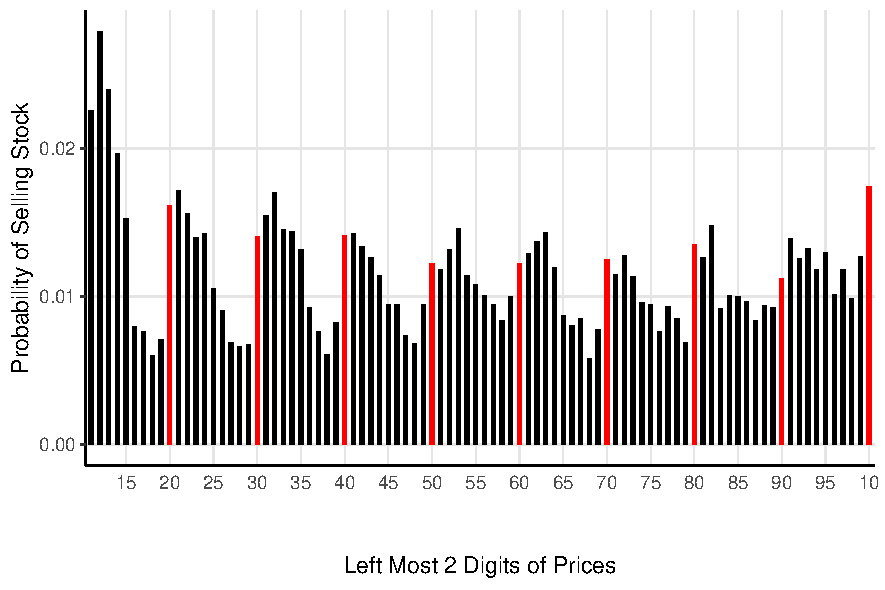
\includegraphics[width=0.65\textwidth]{figures/2left_increase.pdf}
	\fignote{}
\end{figure}

Note above that the 10 bar is the last one, I put it at the end because prices are generally increasing so the 99 bar is usually for prices preceding the 10 bar (e.g., £0.99 increasing to £1.00; £9.9 increasing to £10, etc.).

\begin{figure}[hp]
	\centering%
	\caption{Probability of Selling  for Stocks that Change the First Digit}%
	\label{fig:bars_prob}%
	\subfigure[Stocks with Prices from £0.11 to £1.01 (1p bins)]{	
		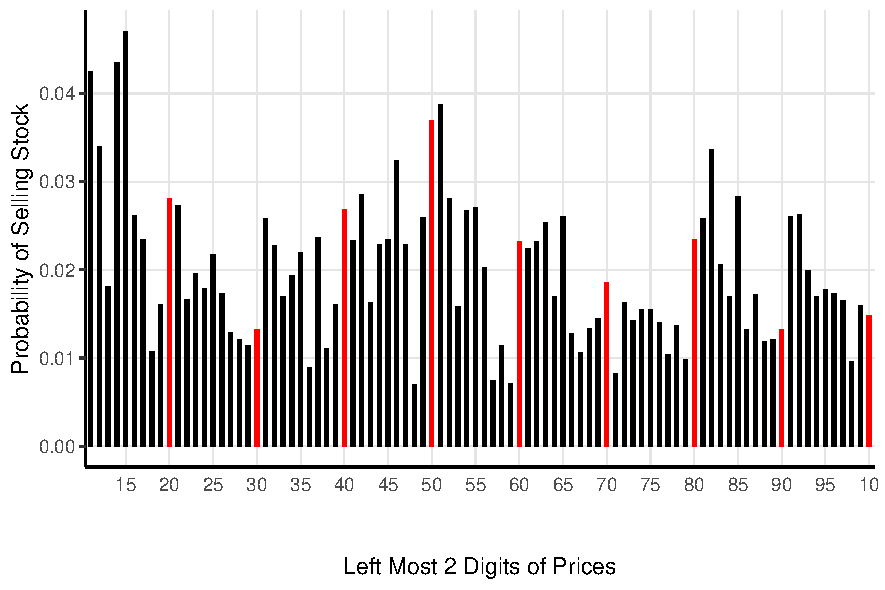
\includegraphics[width=0.65\textwidth]{figures/2left_increase_bin1p.pdf}
	}
	\subfigure[Stocks with Prices from £1.1 to £10.1  (10p  bins)]{	
		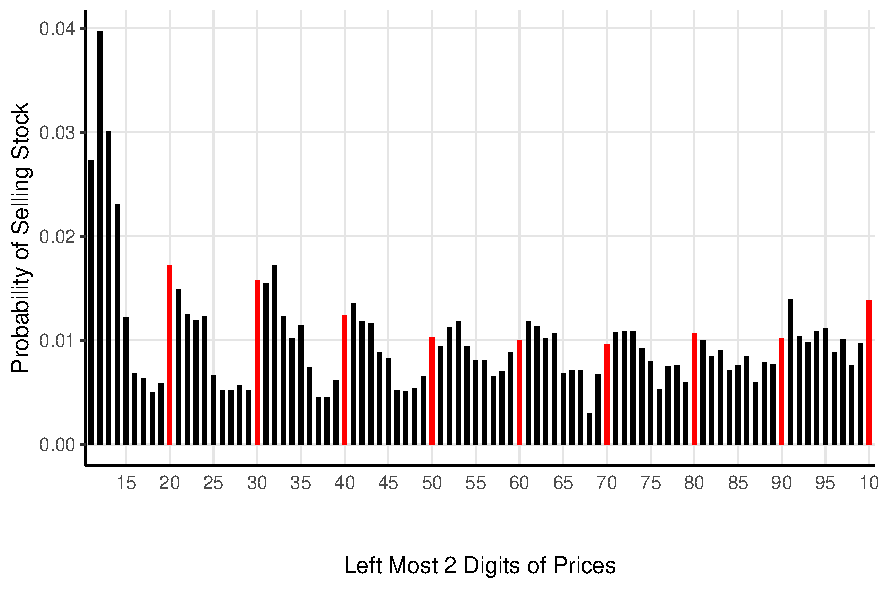
\includegraphics[width=0.65\textwidth]{figures/2left_increase_bin10p.pdf}
	}	
	\subfigure[Stocks with Prices from £11 to £101 
	(£1  bins)]{	
		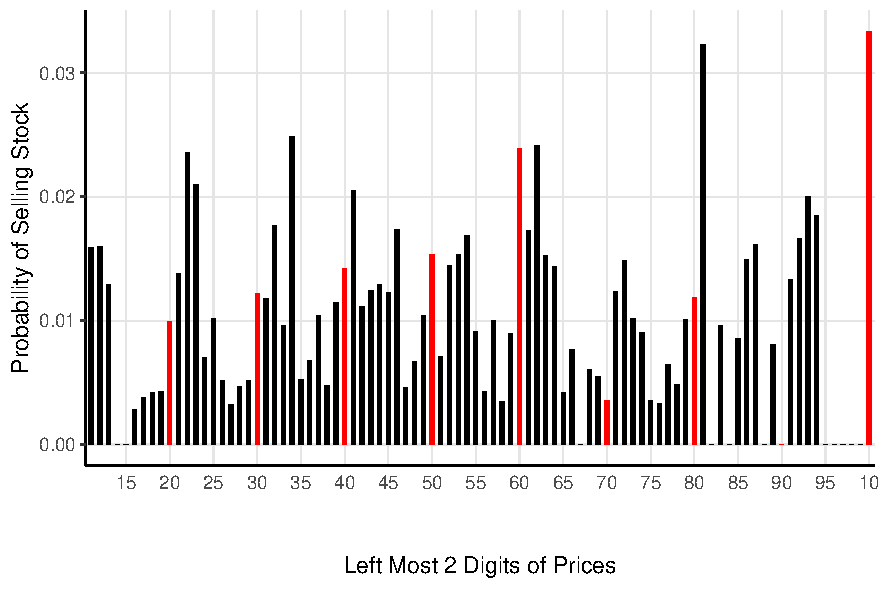
\includegraphics[width=0.65\textwidth]{figures/2left_increase_bin1pound.pdf}
	}	
	\fignote{  }
\end{figure}

\clearpage
\subsubsection{Raw Patterns Showing the Second Digit and the Probability to Sell}


\begin{figure}[hbt!]
	\centering%
	\caption{Probability of Selling  for Stocks that Change the First Digit \\ All Stocks (different bin size)}%
	\label{fig:prob_all_inc}%
	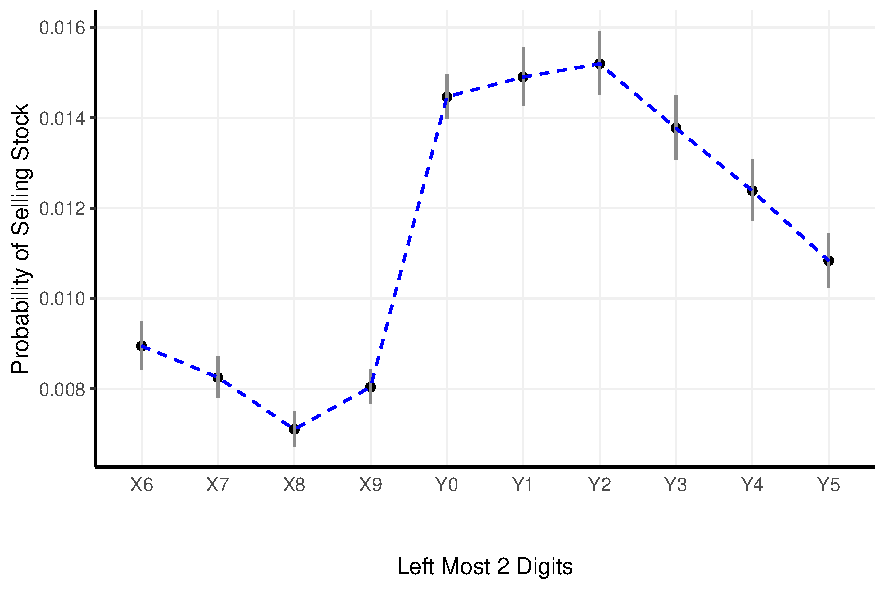
\includegraphics[width=0.65\textwidth]{figures/Left2increase_probCI.pdf}
	\fignote{}
\end{figure}


\begin{figure}[hp]
	\centering%
	\caption{Probability of Selling  for Stocks that Change the First Digit}%
	\label{fig:prob_inc_samples}%
	\subfigure[Stocks with Prices from £0.11 to £1.01 (1p bins)]{	
		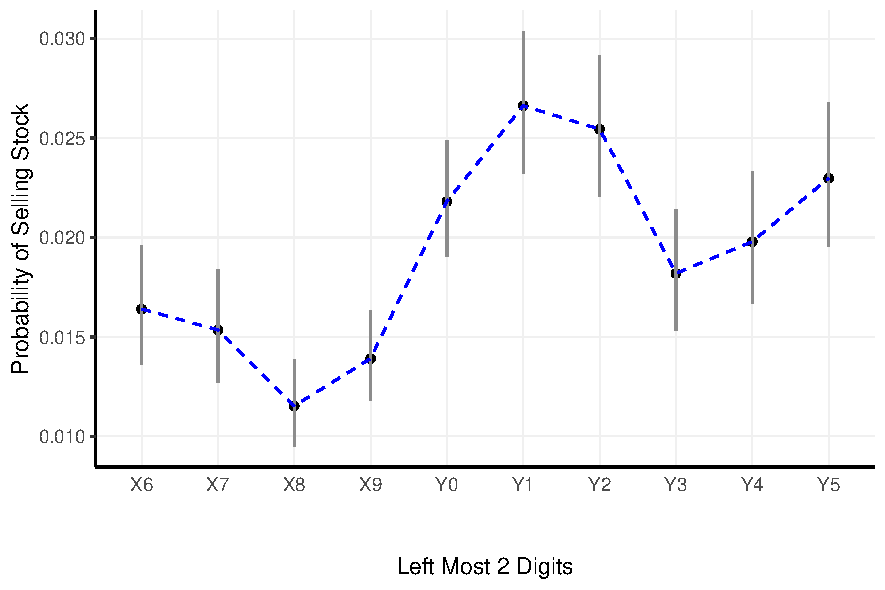
\includegraphics[width=0.65\textwidth]{figures/Left2increases_1pbin_CI.pdf}
	}
	\subfigure[Stocks with Prices from £1.1 to £10.1  (10p  bins)]{	
		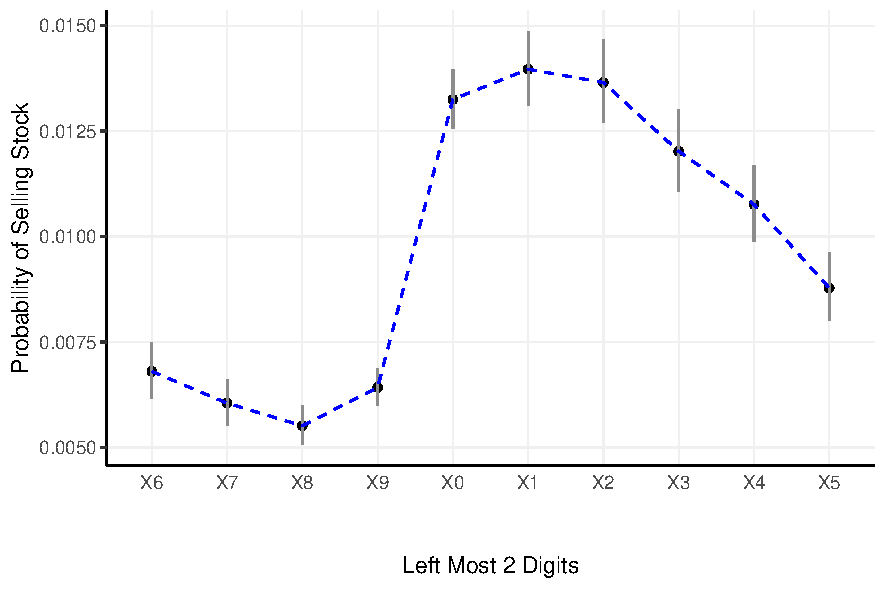
\includegraphics[width=0.65\textwidth]{figures/Left2increases_10pbin_CI.pdf}
	}	
	\subfigure[Stocks with Prices from £11 to £101 
	(£1  bins)]{	
		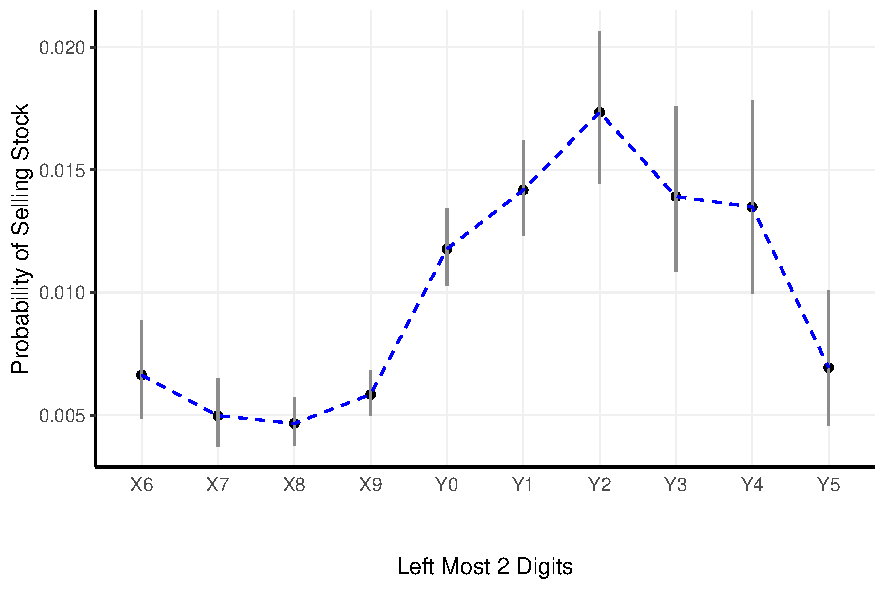
\includegraphics[width=0.65\textwidth]{figures/Left2increases_1poundbin_CI.pdf}
	}	
	\fignote{  }
\end{figure}

\clearpage

\subsubsection{Simulated prices}

I simulated prices for each stock following random walks, ARIMA (1,1,0) and AR=0.7,  and replace the real prices with the simulated ones. Following the same procedure of sample selection, selecting quarters on which the first digit change, we have further evidence that our results are not an artefact of the sample selection. \textcolor{blue}{I think I can try a permutation of all the stocks that people have in their portfolios (so changing the prices of their stocks but with other real stocks' prices), while leaving invariant the sell dummy, and run al the analysis again following all the steps used in the sample restriction. We should not find an effect.}



\begin{figure}[hbt!]
	\centering%
	\caption{Probability of Selling  for Stocks that Change the First Digit \\ All Stocks (different bin size)}%
	\label{fig:}%
	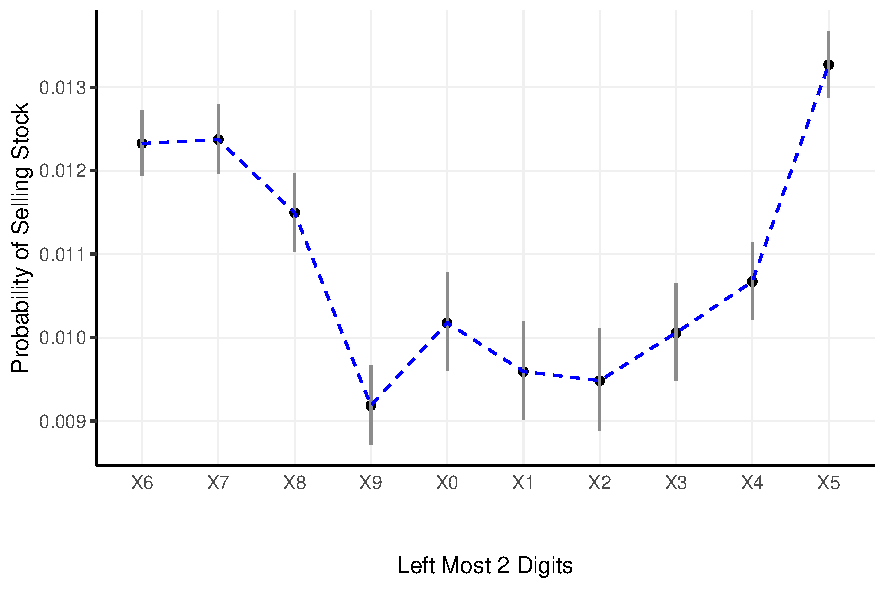
\includegraphics[width=0.65\textwidth]{figures/Left2increase_probCI_random.pdf}
	\fignote{}
\end{figure}


\begin{figure}[hbt!]
	\centering%
	\caption{Probability of Selling  for the Remaining Stocks \\ All Stocks (different bin size)}%
	\label{fig:}%
	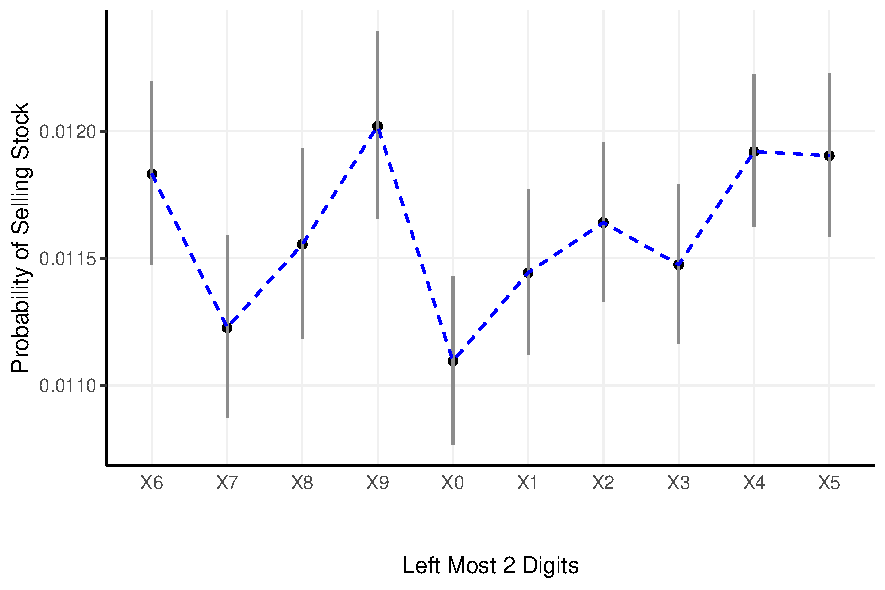
\includegraphics[width=0.65\textwidth]{figures/Left2decrease_probCI_random.pdf}
	\fignote{}
\end{figure}

\clearpage

\subsubsection{Regressions}

Regressions fit an intercept for the change in the left most digit at X0 and two slopes for the left (X6 to X9) and right (X0 to X5) values, as described by the raw patterns in \ref{fig:prob_all_inc}. 
The constant shows the probability to sell the stock at when the second digit is 9 (X9). The second digit over threshold dummy shows the jump in probability when the first digit changes and so the second digit becomes 0 (X0). SE are clustered by account.

\begin{econtable}[h]\footnotesize
	\caption{All Stocks}
	\label{tab:}
	\estauto{l c c c c c c  }{
		& \multicolumn{5}{c}{$Probability\:  of\:  Sale_{ijt}=1$} \\ 
		%	\cmidrule(rr){2-7}
		& \multicolumn{1}{c}{(1)} & \multicolumn{1}{c}{(2)} & \multicolumn{1}{c}{(3)} & \multicolumn{1}{c}{(4)} & 
		\multicolumn{1}{c}{(5)} & \\ 
		\midrule
		\\[-2.1ex] Above X0 = 1 & 0.0058{***} & 0.0076{***} & 0.0070{***} & 0.0067{***} & 0.0070{***} \\ 
  & (0.0002) & (0.0003) & (0.0003) & (0.0003) & (0.0003) \\ 
  Stock Digits (XO to X5) &  & -0.0007{***} & -0.0008{***} & -0.0008{***} & -0.0010{***} \\ 
  &  & (0.0001) & (0.0001) & (0.0001) & (0.0001) \\ 
  Stock Digits (X6 to X9) &  & -0.0003{***} & -0.0001 & -0.0001 & 0.0001 \\ 
  &  & (0.0001) & (0.0001) & (0.0001) & (0.0001) \\ 
  Constant & 0.0080{***} & 0.0076{***} & 0.0098{***} &  &  \\ 
  & (0.0003) & (0.0003) & (0.0025) &  &  \\ 
 Day FE & NO & NO & YES & YES & YES \\ 
Industry FE & NO & NO & YES & YES & YES \\ 
Account FE & NO & NO & NO & YES & YES \\ 
Stock FE & NO & NO & NO & NO & YES \\ 
Observations & \multicolumn{1}{c}{1,517,823} & \multicolumn{1}{c}{1,517,823} & \multicolumn{1}{c}{1,517,823} & \multicolumn{1}{c}{1,517,823} & \multicolumn{1}{c}{1,517,823} \\ 
R$^{2}$ & \multicolumn{1}{c}{0.0008} & \multicolumn{1}{c}{0.0008} & \multicolumn{1}{c}{0.0022} & \multicolumn{1}{c}{0.0511} & \multicolumn{1}{c}{0.0549} \\ 
 
	}
	\fignote{The unit of observation is an investor $\times$ stock $\times$ day. The samples is restricted to login days. We include only quarters in which the stocks increased in price (regarding the first observation of the quarter) and change the left most digit at least once during the quarter. Only those stocks that have changed the left most digit are included. Regressions fit an intercept for the change in the left most digit at X0 and two slopes for the left (X6 to X9) and right (X0 to X5) values, as described by the raw patterns in \ref{fig:prob_all_inc}. The constant shows the probability to sell the stock at when the second digit is 9 (X9). The second digit over threshold dummy shows the jump in probability when the first digit changes and so the second digit becomes 0 (X0). SE are clustered by account.}
\end{econtable}


\begin{econtable}[h]\footnotesize
	\caption{Stocks with Prices Between \pounds 0.11 to \pounds 1.01}
	\label{tab:}
	\estauto{l c c c c c c  }{
		& \multicolumn{5}{c}{$Probability\:  of\:  Sale_{ijt}=1$} \\ 
		%	\cmidrule(rr){2-7}
		& \multicolumn{1}{c}{(1)} & \multicolumn{1}{c}{(2)} & \multicolumn{1}{c}{(3)} & \multicolumn{1}{c}{(4)} & 
		\multicolumn{1}{c}{(5)} & \\ 
		\midrule
		\\[-2.1ex] Second Digit Over Threshold = 1 (in Range X0 to X5) & 0.0046{***} & 0.0069{***} & 0.0061{***} & 0.0057{***} & 0.0055{***} \\ 
  & (0.0004) & (0.0006) & (0.0006) & (0.0006) & (0.0006) \\ 
  Second Digit Over Threshold (= 0 to 5, corresponding to X0 to X5) &  & -0.0007{***} & -0.0007{***} & -0.0006{***} & -0.0006{***} \\ 
  &  & (0.0002) & (0.0002) & (0.0002) & (0.0002) \\ 
  Second Digit Below Threshold (= -3 to 0, corresponding to X6 to X9) &  & -0.0004{*} & -0.0003 & -0.0004{*} & -0.0004 \\ 
  &  & (0.0002) & (0.0002) & (0.0002) & (0.0002) \\ 
  Constant & 0.0094{***} & 0.0088{***} & 0.0687{***} &  &  \\ 
  & (0.0004) & (0.0005) & (0.0262) &  &  \\ 
 Day FE & NO & NO & YES & YES & YES \\ 
Industry FE & NO & NO & YES & YES & YES \\ 
Account FE & NO & NO & NO & YES & YES \\ 
Stock FE & NO & NO & NO & NO & YES \\ 
Observations & \multicolumn{1}{c}{387,060} & \multicolumn{1}{c}{387,060} & \multicolumn{1}{c}{387,060} & \multicolumn{1}{c}{387,060} & \multicolumn{1}{c}{387,060} \\ 
R$^{2}$ & \multicolumn{1}{c}{0.0005} & \multicolumn{1}{c}{0.0005} & \multicolumn{1}{c}{0.0023} & \multicolumn{1}{c}{0.0756} & \multicolumn{1}{c}{0.0800} \\ 
 
	}
	\fignote{The unit of observation is an investor $\times$ stock $\times$ day. The samples is restricted to login days. We include only quarters in which the stocks increased in price (regarding the first observation of the quarter) and change the left most digit at least once during the quarter. Only those stocks that have changed the left most digit are included. Regressions fit an intercept for the change in the left most digit at X0 and two slopes for the left (X6 to X9) and right (X0 to X5) values, as described by the raw patterns in \ref{fig:prob_inc_samples}. The constant shows the probability to sell the stock at when the second digit is 9 (X9). The second digit over threshold dummy shows the jump in probability when the first digit changes and so the second digit becomes 0 (X0). SE are clustered by account.}
\end{econtable}


\begin{econtable}[h]\footnotesize
	\caption{Stocks with Prices Between \pounds 1.1 to \pounds 10.1}
	\label{tab:}
	\estauto{l c c c c c c  }{
		& \multicolumn{5}{c}{$Probability\:  of\:  Sale_{ijt}=1$} \\ 
		%	\cmidrule(rr){2-7}
		& \multicolumn{1}{c}{(1)} & \multicolumn{1}{c}{(2)} & \multicolumn{1}{c}{(3)} & \multicolumn{1}{c}{(4)} & 
		\multicolumn{1}{c}{(5)} & \\ 
		\midrule
		 Above Y0 = 1 (in Range Y0 to Y5) & 0.0098{***} & 0.0116{***} & 0.0114{***} & 0.0123{***} & 0.0124{***} \\ 
  & (0.0007) & (0.0010) & (0.0010) & (0.0010) & (0.0011) \\ 
  Stock Digits Y0 to Y5 &  & -0.0007{**} & -0.0012{***} & -0.0008{***} & -0.0010{***} \\ 
  &  & (0.0003) & (0.0003) & (0.0003) & (0.0003) \\ 
  Stock Digits X6 to X9 &  & -0.0004 & 0.0001 & -0.0003 & -0.0001 \\ 
  &  & (0.0004) & (0.0004) & (0.0004) & (0.0004) \\ 
  Constant & 0.0097{***} & 0.0093{***} & 0.0433{***} &  &  \\ 
  & (0.0005) & (0.0007) & (0.0041) &  &  \\ 
 Day FE & NO & NO & YES & YES & YES \\ 
Industry FE & NO & NO & YES & YES & YES \\ 
Account FE & NO & NO & NO & YES & YES \\ 
Stock FE & NO & NO & NO & NO & YES \\ 
Observations & \multicolumn{1}{c}{155,842} & \multicolumn{1}{c}{155,842} & \multicolumn{1}{c}{155,842} & \multicolumn{1}{c}{155,842} & \multicolumn{1}{c}{155,842} \\ 
R$^{2}$ & \multicolumn{1}{c}{0.0016} & \multicolumn{1}{c}{0.0016} & \multicolumn{1}{c}{0.0058} & \multicolumn{1}{c}{0.1185} & \multicolumn{1}{c}{0.1271} \\ 
 
	}
	\fignote{The unit of observation is an investor $\times$ stock $\times$ day. The samples is restricted to login days. We include only quarters in which the stocks increased in price (regarding the first observation of the quarter) and change the left most digit at least once during the quarter. Only those stocks that have changed the left most digit are included. Regressions fit an intercept for the change in the left most digit at X0 and two slopes for the left (X6 to X9) and right (X0 to X5) values, as described by the raw patterns in \ref{fig:prob_inc_samples}. The constant shows the probability to sell the stock at when the second digit is 9 (X9). The second digit over threshold dummy shows the jump in probability when the first digit changes and so the second digit becomes 0 (X0). SE are clustered by account.}
\end{econtable}

\begin{econtable}[h]\footnotesize
	\caption{Stocks with Prices Between \pounds 11 to \pounds 101}
	\label{tab:}
	\estauto{l c c c c c c  }{
		& \multicolumn{5}{c}{$Probability\:  of\:  Sale_{ijt}=1$} \\ 
		%	\cmidrule(rr){2-7}
		& \multicolumn{1}{c}{(1)} & \multicolumn{1}{c}{(2)} & \multicolumn{1}{c}{(3)} & \multicolumn{1}{c}{(4)} & 
		\multicolumn{1}{c}{(5)} & \\ 
		\midrule
		 Above Y0 = 1 (in Range Y0 to Y5) & 0.0112{***} & 0.0133{***} & 0.0132{***} & 0.0163{***} & 0.0171{***} \\ 
  & (0.0016) & (0.0022) & (0.0022) & (0.0028) & (0.0028) \\ 
  Stock Digits Y0 to Y5 &  & -0.0005 & -0.0004 & 0.0008 & 0.0011 \\ 
  &  & (0.0008) & (0.0009) & (0.0009) & (0.0010) \\ 
  Stock Digits X6 to X9 &  & -0.0017 & -0.0018 & -0.0016 & -0.0021 \\ 
  &  & (0.0013) & (0.0013) & (0.0014) & (0.0015) \\ 
  Constant & 0.0106{***} & 0.0092{***} & 0.0245{***} &  &  \\ 
  & (0.0012) & (0.0014) & (0.0047) &  &  \\ 
 Day FE & NO & NO & YES & YES & YES \\ 
Industry FE & NO & NO & YES & YES & YES \\ 
Account FE & NO & NO & NO & YES & YES \\ 
Stock FE & NO & NO & NO & NO & YES \\ 
Observations & \multicolumn{1}{c}{25,401} & \multicolumn{1}{c}{25,401} & \multicolumn{1}{c}{25,401} & \multicolumn{1}{c}{25,401} & \multicolumn{1}{c}{25,401} \\ 
R$^{2}$ & \multicolumn{1}{c}{0.0017} & \multicolumn{1}{c}{0.0018} & \multicolumn{1}{c}{0.0042} & \multicolumn{1}{c}{0.1850} & \multicolumn{1}{c}{0.1968} \\ 
 
	}
	\fignote{The unit of observation is an investor $\times$ stock $\times$ day. The samples is restricted to login days. We include only quarters in which the stocks increased in price (regarding the first observation of the quarter) and change the left most digit at least once during the quarter. Only those stocks that have changed the left most digit are included. Regressions fit an intercept for the change in the left most digit at X0 and two slopes for the left (X6 to X9) and right (X0 to X5) values, as described by the raw patterns in \ref{fig:prob_inc_samples}. The constant shows the probability to sell the stock at when the second digit is 9 (X9). The second digit over threshold dummy shows the jump in probability when the first digit changes and so the second digit becomes 0 (X0). SE are clustered by account.}
\end{econtable}

\clearpage


\subsubsection{\textcolor{blue}{Regressions - Highest Quartile of Stocks Based on Volatility}}

\textcolor{blue}{Results from this section should be compared with regression results from the earlier section 1.2.4. We might expect that coefficients using a sample of stocks that are highly volatile would have bigger coefficients for the dummy of the second digit.}



Regressions fit an intercept for the change in the left most digit at X0 and two slopes for the left (X6 to X9) and right (X0 to X5) values, as described by the raw patterns in \ref{fig:all_obs}. 
The constant shows the probability to sell the stock at when the second digit is 9 (X9). The second digit over threshold dummy shows the jump in probability when the first digit changes and so the second digit becomes 0 (X0). SE are clustered by account.

\begin{econtable}[h]\footnotesize
	\caption{All Stocks}
	\label{tab:}
	\estauto{l c c c c c c  }{
		& \multicolumn{5}{c}{$Probability\:  of\:  Sale_{ijt}=1$} \\ 
		%	\cmidrule(rr){2-7}
		& \multicolumn{1}{c}{(1)} & \multicolumn{1}{c}{(2)} & \multicolumn{1}{c}{(3)} & \multicolumn{1}{c}{(4)} & 
		\multicolumn{1}{c}{(5)} & \\ 
		\midrule
		 Second Digit Over Threshold = 1 (in Range X0 to X5) & 0.0045{***} & 0.0052{***} & 0.0051{***} & 0.0053{***} & 0.0057{***} \\ 
  & (0.0004) & (0.0007) & (0.0007) & (0.0007) & (0.0007) \\ 
  Second Digit Over Threshold (= 0 to 5, corresponding to X0 to X5) &  & -0.0006{***} & -0.0007{***} & -0.0007{***} & -0.0008{***} \\ 
  &  & (0.0002) & (0.0002) & (0.0001) & (0.0001) \\ 
  Second Digit Below Threshold (= -3 to 0, corresponding to X6 to X9) &  & 0.0004 & 0.0005{*} & 0.0002 & 0.0001 \\ 
  &  & (0.0002) & (0.0002) & (0.0002) & (0.0002) \\ 
  Constant & 0.0140{***} & 0.0146{***} & 0.0116{***} &  &  \\ 
  & (0.0006) & (0.0007) & (0.0025) &  &  \\ 
 Day FE & NO & NO & YES & YES & YES \\ 
Industry FE & NO & NO & YES & YES & YES \\ 
Account FE & NO & NO & NO & YES & YES \\ 
Stock FE & NO & NO & NO & NO & YES \\ 
Observations & \multicolumn{1}{c}{534,511} & \multicolumn{1}{c}{534,511} & \multicolumn{1}{c}{534,511} & \multicolumn{1}{c}{534,511} & \multicolumn{1}{c}{534,511} \\ 
R$^{2}$ & \multicolumn{1}{c}{0.0003} & \multicolumn{1}{c}{0.0003} & \multicolumn{1}{c}{0.0009} & \multicolumn{1}{c}{0.0687} & \multicolumn{1}{c}{0.0731} \\ 
 
	}
	\fignote{The unit of observation is an investor $\times$ stock $\times$ day. The samples is restricted to login days. We include only quarters in which the stocks increased in price (regarding the first observation of the quarter) and change the left most digit at least once during the quarter. Only those stocks that have changed the left most digit are included. Regressions fit an intercept for the change in the left most digit at X0 and two slopes for the left (X6 to X9) and right (X0 to X5) values, as described by the raw patterns in \ref{fig:prob_all_inc}. The constant shows the probability to sell the stock at when the second digit is 9 (X9). The second digit over threshold dummy shows the jump in probability when the first digit changes and so the second digit becomes 0 (X0). SE are clustered by account.}
\end{econtable}


\begin{econtable}[h]\footnotesize
	\caption{Stocks with Prices Between \pounds 0.11 to \pounds 1.01}
	\label{tab:}
	\estauto{l c c c c c c  }{
		& \multicolumn{5}{c}{$Probability\:  of\:  Sale_{ijt}=1$} \\ 
		%	\cmidrule(rr){2-7}
		& \multicolumn{1}{c}{(1)} & \multicolumn{1}{c}{(2)} & \multicolumn{1}{c}{(3)} & \multicolumn{1}{c}{(4)} & 
		\multicolumn{1}{c}{(5)} & \\ 
		\midrule
		 Second Digit Over Threshold = 1 (in Range X0 to X5) & 0.0042{***} & 0.0055{***} & 0.0052{***} & 0.0047{***} & 0.0043{***} \\ 
  & (0.0006) & (0.0010) & (0.0010) & (0.0010) & (0.0010) \\ 
  Second Digit Over Threshold (= 0 to 5, corresponding to X0 to X5) &  & -0.0005{**} & -0.0005{**} & -0.0004 & -0.0004 \\ 
  &  & (0.0002) & (0.0002) & (0.0002) & (0.0002) \\ 
  Second Digit Below Threshold (= -3 to 0, corresponding to X6 to X9) &  & -0.0001 & 0.0000 & -0.0002 & -0.0001 \\ 
  &  & (0.0004) & (0.0004) & (0.0004) & (0.0004) \\ 
  Constant & 0.0135{***} & 0.0135{***} & 0.0692{***} &  &  \\ 
  & (0.0008) & (0.0009) & (0.0262) &  &  \\ 
 Day FE & NO & NO & YES & YES & YES \\ 
Industry FE & NO & NO & YES & YES & YES \\ 
Account FE & NO & NO & NO & YES & YES \\ 
Stock FE & NO & NO & NO & NO & YES \\ 
Observations & \multicolumn{1}{c}{194,573} & \multicolumn{1}{c}{194,573} & \multicolumn{1}{c}{194,573} & \multicolumn{1}{c}{194,573} & \multicolumn{1}{c}{194,573} \\ 
R$^{2}$ & \multicolumn{1}{c}{0.0003} & \multicolumn{1}{c}{0.0003} & \multicolumn{1}{c}{0.0015} & \multicolumn{1}{c}{0.0936} & \multicolumn{1}{c}{0.0989} \\ 
 
	}
	\fignote{The unit of observation is an investor $\times$ stock $\times$ day. The samples is restricted to login days. We include only quarters in which the stocks increased in price (regarding the first observation of the quarter) and change the left most digit at least once during the quarter. Only those stocks that have changed the left most digit are included. Regressions fit an intercept for the change in the left most digit at X0 and two slopes for the left (X6 to X9) and right (X0 to X5) values, as described by the raw patterns in \ref{fig:prob_inc_samples}. The constant shows the probability to sell the stock at when the second digit is 9 (X9). The second digit over threshold dummy shows the jump in probability when the first digit changes and so the second digit becomes 0 (X0). SE are clustered by account.}
\end{econtable}


\begin{econtable}[h]\footnotesize
	\caption{Stocks with Prices Between \pounds 1.1 to \pounds 10.1}
	\label{tab:}
	\estauto{l c c c c c c  }{
		& \multicolumn{5}{c}{$Probability\:  of\:  Sale_{ijt}=1$} \\ 
		%	\cmidrule(rr){2-7}
		& \multicolumn{1}{c}{(1)} & \multicolumn{1}{c}{(2)} & \multicolumn{1}{c}{(3)} & \multicolumn{1}{c}{(4)} & 
		\multicolumn{1}{c}{(5)} & \\ 
		\midrule
		 Second Digit Over Threshold = 1 (in Range X0 to X5) & 0.0108{***} & 0.0135{***} & 0.0129{***} & 0.0113{***} & 0.0109{***} \\ 
  & (0.0010) & (0.0015) & (0.0015) & (0.0015) & (0.0015) \\ 
  Second Digit Over Threshold (= 0 to 5, corresponding to X0 to X5) &  & -0.0009{**} & -0.0010{***} & -0.0011{***} & -0.0010{***} \\ 
  &  & (0.0004) & (0.0004) & (0.0004) & (0.0004) \\ 
  Second Digit Below Threshold (= -3 to 0, corresponding to X6 to X9) &  & -0.0005 & -0.0003 & -0.0005 & -0.0005 \\ 
  &  & (0.0006) & (0.0006) & (0.0005) & (0.0005) \\ 
  Constant & 0.0121{***} & 0.0113{***} & 0.0187{***} &  &  \\ 
  & (0.0010) & (0.0012) & (0.0026) &  &  \\ 
 Day FE & NO & NO & YES & YES & YES \\ 
Industry FE & NO & NO & YES & YES & YES \\ 
Account FE & NO & NO & NO & YES & YES \\ 
Stock FE & NO & NO & NO & NO & YES \\ 
Observations & \multicolumn{1}{c}{103,156} & \multicolumn{1}{c}{103,156} & \multicolumn{1}{c}{103,156} & \multicolumn{1}{c}{103,156} & \multicolumn{1}{c}{103,156} \\ 
R$^{2}$ & \multicolumn{1}{c}{0.0016} & \multicolumn{1}{c}{0.0017} & \multicolumn{1}{c}{0.0034} & \multicolumn{1}{c}{0.1335} & \multicolumn{1}{c}{0.1376} \\ 
 
	}
	\fignote{The unit of observation is an investor $\times$ stock $\times$ day. The samples is restricted to login days. We include only quarters in which the stocks increased in price (regarding the first observation of the quarter) and change the left most digit at least once during the quarter. Only those stocks that have changed the left most digit are included. Regressions fit an intercept for the change in the left most digit at X0 and two slopes for the left (X6 to X9) and right (X0 to X5) values, as described by the raw patterns in \ref{fig:prob_inc_samples}. The constant shows the probability to sell the stock at when the second digit is 9 (X9). The second digit over threshold dummy shows the jump in probability when the first digit changes and so the second digit becomes 0 (X0). SE are clustered by account.}
\end{econtable}

\begin{econtable}[h]\footnotesize
	\caption{Stocks with Prices Between \pounds 11 to \pounds 101}
	\label{tab:}
	\estauto{l c c c c c c  }{
		& \multicolumn{5}{c}{$Probability\:  of\:  Sale_{ijt}=1$} \\ 
		%	\cmidrule(rr){2-7}
		& \multicolumn{1}{c}{(1)} & \multicolumn{1}{c}{(2)} & \multicolumn{1}{c}{(3)} & \multicolumn{1}{c}{(4)} & 
		\multicolumn{1}{c}{(5)} & \\ 
		\midrule
		 Second Digit Over Threshold = 1 (in Range X0 to X5) & 0.0047{*} & 0.0101{**} & 0.0085{**} & 0.0065 & 0.0061 \\ 
  & (0.0025) & (0.0042) & (0.0043) & (0.0045) & (0.0045) \\ 
  Second Digit Over Threshold (= 0 to 5, corresponding to X0 to X5) &  & -0.0022{*} & -0.0019 & -0.0012 & -0.0010 \\ 
  &  & (0.0013) & (0.0014) & (0.0014) & (0.0013) \\ 
  Second Digit Below Threshold (= -3 to 0, corresponding to X6 to X9) &  & -0.0005 & -0.0007 & -0.0012 & -0.0012 \\ 
  &  & (0.0015) & (0.0015) & (0.0016) & (0.0016) \\ 
  Constant & 0.0116{***} & 0.0109{***} & 0.0151 &  &  \\ 
  & (0.0024) & (0.0030) & (0.0092) &  &  \\ 
 Day FE & NO & NO & YES & YES & YES \\ 
Industry FE & NO & NO & YES & YES & YES \\ 
Account FE & NO & NO & NO & YES & YES \\ 
Stock FE & NO & NO & NO & NO & YES \\ 
Observations & \multicolumn{1}{c}{8,949} & \multicolumn{1}{c}{8,949} & \multicolumn{1}{c}{8,949} & \multicolumn{1}{c}{8,949} & \multicolumn{1}{c}{8,949} \\ 
R$^{2}$ & \multicolumn{1}{c}{0.0004} & \multicolumn{1}{c}{0.0009} & \multicolumn{1}{c}{0.0035} & \multicolumn{1}{c}{0.1034} & \multicolumn{1}{c}{0.1129} \\ 
 
	}
	\fignote{The unit of observation is an investor $\times$ stock $\times$ day. The samples is restricted to login days. We include only quarters in which the stocks increased in price (regarding the first observation of the quarter) and change the left most digit at least once during the quarter. Only those stocks that have changed the left most digit are included. Regressions fit an intercept for the change in the left most digit at X0 and two slopes for the left (X6 to X9) and right (X0 to X5) values, as described by the raw patterns in \ref{fig:prob_inc_samples}. The constant shows the probability to sell the stock at when the second digit is 9 (X9). The second digit over threshold dummy shows the jump in probability when the first digit changes and so the second digit becomes 0 (X0). SE are clustered by account.}
\end{econtable}

\clearpage




\subsubsection{\textcolor{blue}{Regressions - Lowest Quartile of Stocks Based on Volatility}}

\textcolor{blue}{Results from this section should be compared with regression results from the earlier section 1.2.4. We might expect that coefficients using a sample of stocks that have low volatility would have smaller coefficients for the dummy of the second digit. But the coefficients are still significant and precisely estimated }



Regressions fit an intercept for the change in the left most digit at X0 and two slopes for the left (X6 to X9) and right (X0 to X5) values, as described by the raw patterns in \ref{fig:prob_all_inc}. 
The constant shows the probability to sell the stock at when the second digit is 9 (X9). The second digit over threshold dummy shows the jump in probability when the first digit changes and so the second digit becomes 0 (X0). SE are clustered by account.

\begin{econtable}[h]\footnotesize
	\caption{All Stocks}
	\label{tab:}
	\estauto{l c c c c c c  }{
		& \multicolumn{5}{c}{$Probability\:  of\:  Sale_{ijt}=1$} \\ 
		%	\cmidrule(rr){2-7}
		& \multicolumn{1}{c}{(1)} & \multicolumn{1}{c}{(2)} & \multicolumn{1}{c}{(3)} & \multicolumn{1}{c}{(4)} & 
		\multicolumn{1}{c}{(5)} & \\ 
		\midrule
		 Second Digit Over Threshold = 1 (in Range X0 to X5) & 0.0047{***} & 0.0050{***} & 0.0050{***} & 0.0050{***} & 0.0053{***} \\ 
  & (0.0004) & (0.0005) & (0.0005) & (0.0005) & (0.0005) \\ 
  Second Digit Over Threshold (= 0 to 5, corresponding to X0 to X5) &  & -0.0002 & -0.0002 & -0.0001 & -0.0002 \\ 
  &  & (0.0001) & (0.0001) & (0.0001) & (0.0002) \\ 
  Second Digit Below Threshold (= -3 to 0, corresponding to X6 to X9) &  & -0.0001 & -0.0001 & -0.0002 & -0.0000 \\ 
  &  & (0.0002) & (0.0002) & (0.0002) & (0.0002) \\ 
  Constant & 0.0032{***} & 0.0031{***} & 0.0119 &  &  \\ 
  & (0.0002) & (0.0003) & (0.0087) &  &  \\ 
 Day FE & NO & NO & YES & YES & YES \\ 
Industry FE & NO & NO & YES & YES & YES \\ 
Account FE & NO & NO & NO & YES & YES \\ 
Stock FE & NO & NO & NO & NO & YES \\ 
Observations & \multicolumn{1}{c}{220,953} & \multicolumn{1}{c}{220,953} & \multicolumn{1}{c}{220,953} & \multicolumn{1}{c}{220,953} & \multicolumn{1}{c}{220,953} \\ 
R$^{2}$ & \multicolumn{1}{c}{0.0010} & \multicolumn{1}{c}{0.0010} & \multicolumn{1}{c}{0.0013} & \multicolumn{1}{c}{0.0506} & \multicolumn{1}{c}{0.0536} \\ 
 
	}
	\fignote{The unit of observation is an investor $\times$ stock $\times$ day. The samples is restricted to login days. We include only quarters in which the stocks increased in price (regarding the first observation of the quarter) and change the left most digit at least once during the quarter. Only those stocks that have changed the left most digit are included. Regressions fit an intercept for the change in the left most digit at X0 and two slopes for the left (X6 to X9) and right (X0 to X5) values, as described by the raw patterns in \ref{fig:prob_all_inc}. The constant shows the probability to sell the stock at when the second digit is 9 (X9). The second digit over threshold dummy shows the jump in probability when the first digit changes and so the second digit becomes 0 (X0). SE are clustered by account.}
\end{econtable}


\begin{econtable}[h]\footnotesize
	\caption{Stocks with Prices Between \pounds 0.11 to \pounds 1.01}
	\label{tab:}
	\estauto{l c c c c c c  }{
		& \multicolumn{5}{c}{$Probability\:  of\:  Sale_{ijt}=1$} \\ 
		%	\cmidrule(rr){2-7}
		& \multicolumn{1}{c}{(1)} & \multicolumn{1}{c}{(2)} & \multicolumn{1}{c}{(3)} & \multicolumn{1}{c}{(4)} & 
		\multicolumn{1}{c}{(5)} & \\ 
		\midrule
		 Second Digit Over Threshold = 1 (in Range X0 to X5) & 0.0018{**} & 0.0018{*} & 0.0019{**} & 0.0017{*} & 0.0019{*} \\ 
  & (0.0008) & (0.0009) & (0.0009) & (0.0010) & (0.0010) \\ 
  Second Digit Over Threshold (= 0 to 5, corresponding to X0 to X5) &  & 0.0001 & 0.0001 & 0.0002 & 0.0001 \\ 
  &  & (0.0003) & (0.0003) & (0.0003) & (0.0004) \\ 
  Second Digit Below Threshold (= -3 to 0, corresponding to X6 to X9) &  & -0.0001 & -0.0001 & -0.0003 & -0.0003 \\ 
  &  & (0.0004) & (0.0004) & (0.0004) & (0.0004) \\ 
  Constant & 0.0027{***} & 0.0026{***} & -0.0014{**} &  &  \\ 
  & (0.0005) & (0.0006) & (0.0006) &  &  \\ 
 Day FE & NO & NO & YES & YES & YES \\ 
Industry FE & NO & NO & YES & YES & YES \\ 
Account FE & NO & NO & NO & YES & YES \\ 
Stock FE & NO & NO & NO & NO & YES \\ 
Observations & \multicolumn{1}{c}{32,584} & \multicolumn{1}{c}{32,584} & \multicolumn{1}{c}{32,584} & \multicolumn{1}{c}{32,584} & \multicolumn{1}{c}{32,584} \\ 
R$^{2}$ & \multicolumn{1}{c}{0.0002} & \multicolumn{1}{c}{0.0002} & \multicolumn{1}{c}{0.0012} & \multicolumn{1}{c}{0.0541} & \multicolumn{1}{c}{0.0611} \\ 
 
	}
	\fignote{The unit of observation is an investor $\times$ stock $\times$ day. The samples is restricted to login days. We include only quarters in which the stocks increased in price (regarding the first observation of the quarter) and change the left most digit at least once during the quarter. Only those stocks that have changed the left most digit are included. Regressions fit an intercept for the change in the left most digit at X0 and two slopes for the left (X6 to X9) and right (X0 to X5) values, as described by the raw patterns in \ref{fig:prob_inc_samples}. The constant shows the probability to sell the stock at when the second digit is 9 (X9). The second digit over threshold dummy shows the jump in probability when the first digit changes and so the second digit becomes 0 (X0). SE are clustered by account.}
\end{econtable}


\begin{econtable}[h]\footnotesize
	\caption{Stocks with Prices Between \pounds 1.1 to \pounds 10.1}
	\label{tab:}
	\estauto{l c c c c c c  }{
		& \multicolumn{5}{c}{$Probability\:  of\:  Sale_{ijt}=1$} \\ 
		%	\cmidrule(rr){2-7}
		& \multicolumn{1}{c}{(1)} & \multicolumn{1}{c}{(2)} & \multicolumn{1}{c}{(3)} & \multicolumn{1}{c}{(4)} & 
		\multicolumn{1}{c}{(5)} & \\ 
		\midrule
		 Second Digit Over Threshold = 1 (in Range X0 to X5) & 0.0056{***} & 0.0060{***} & 0.0060{***} & 0.0061{***} & 0.0061{***} \\ 
  & (0.0005) & (0.0006) & (0.0006) & (0.0007) & (0.0007) \\ 
  Second Digit Over Threshold (= 0 to 5, corresponding to X0 to X5) &  & -0.0003 & -0.0003 & -0.0002 & -0.0002 \\ 
  &  & (0.0002) & (0.0002) & (0.0002) & (0.0002) \\ 
  Second Digit Below Threshold (= -3 to 0, corresponding to X6 to X9) &  & -0.0000 & -0.0000 & 0.0001 & 0.0002 \\ 
  &  & (0.0002) & (0.0002) & (0.0002) & (0.0003) \\ 
  Constant & 0.0029{***} & 0.0029{***} & 0.0015 &  &  \\ 
  & (0.0003) & (0.0003) & (0.0040) &  &  \\ 
 Day FE & NO & NO & YES & YES & YES \\ 
Industry FE & NO & NO & YES & YES & YES \\ 
Account FE & NO & NO & NO & YES & YES \\ 
Stock FE & NO & NO & NO & NO & YES \\ 
Observations & \multicolumn{1}{c}{144,661} & \multicolumn{1}{c}{144,661} & \multicolumn{1}{c}{144,661} & \multicolumn{1}{c}{144,661} & \multicolumn{1}{c}{144,661} \\ 
R$^{2}$ & \multicolumn{1}{c}{0.0013} & \multicolumn{1}{c}{0.0014} & \multicolumn{1}{c}{0.0016} & \multicolumn{1}{c}{0.0550} & \multicolumn{1}{c}{0.0598} \\ 
 
	}
	\fignote{The unit of observation is an investor $\times$ stock $\times$ day. The samples is restricted to login days. We include only quarters in which the stocks increased in price (regarding the first observation of the quarter) and change the left most digit at least once during the quarter. Only those stocks that have changed the left most digit are included. Regressions fit an intercept for the change in the left most digit at X0 and two slopes for the left (X6 to X9) and right (X0 to X5) values, as described by the raw patterns in \ref{fig:prob_inc_samples}. The constant shows the probability to sell the stock at when the second digit is 9 (X9). The second digit over threshold dummy shows the jump in probability when the first digit changes and so the second digit becomes 0 (X0). SE are clustered by account.}
\end{econtable}

\begin{econtable}[h]\footnotesize
	\caption{Stocks with Prices Between \pounds 11 to \pounds 101}
	\label{tab:}
	\estauto{l c c c c c c  }{
		& \multicolumn{5}{c}{$Probability\:  of\:  Sale_{ijt}=1$} \\ 
		%	\cmidrule(rr){2-7}
		& \multicolumn{1}{c}{(1)} & \multicolumn{1}{c}{(2)} & \multicolumn{1}{c}{(3)} & \multicolumn{1}{c}{(4)} & 
		\multicolumn{1}{c}{(5)} & \\ 
		\midrule
		 Second Digit Over Threshold = 1 (in Range X0 to X5) & 0.0045{***} & 0.0054{***} & 0.0053{***} & 0.0042{***} & 0.0043{***} \\ 
  & (0.0010) & (0.0012) & (0.0012) & (0.0013) & (0.0013) \\ 
  Second Digit Over Threshold (= 0 to 5, corresponding to X0 to X5) &  & -0.0004 & -0.0005 & 0.0003 & 0.0003 \\ 
  &  & (0.0005) & (0.0005) & (0.0005) & (0.0005) \\ 
  Second Digit Below Threshold (= -3 to 0, corresponding to X6 to X9) &  & -0.0007 & -0.0007 & -0.0011 & -0.0011 \\ 
  &  & (0.0007) & (0.0007) & (0.0008) & (0.0008) \\ 
  Constant & 0.0044{***} & 0.0038{***} & 0.0031{***} &  &  \\ 
  & (0.0005) & (0.0007) & (0.0009) &  &  \\ 
 Day FE & NO & NO & YES & YES & YES \\ 
Industry FE & NO & NO & YES & YES & YES \\ 
Account FE & NO & NO & NO & YES & YES \\ 
Stock FE & NO & NO & NO & NO & YES \\ 
Observations & \multicolumn{1}{c}{35,305} & \multicolumn{1}{c}{35,305} & \multicolumn{1}{c}{35,305} & \multicolumn{1}{c}{35,305} & \multicolumn{1}{c}{35,305} \\ 
R$^{2}$ & \multicolumn{1}{c}{0.0008} & \multicolumn{1}{c}{0.0009} & \multicolumn{1}{c}{0.0012} & \multicolumn{1}{c}{0.0843} & \multicolumn{1}{c}{0.0850} \\ 
 
	}
	\fignote{The unit of observation is an investor $\times$ stock $\times$ day. The samples is restricted to login days. We include only quarters in which the stocks increased in price (regarding the first observation of the quarter) and change the left most digit at least once during the quarter. Only those stocks that have changed the left most digit are included. Regressions fit an intercept for the change in the left most digit at X0 and two slopes for the left (X6 to X9) and right (X0 to X5) values, as described by the raw patterns in \ref{fig:prob_inc_samples}. The constant shows the probability to sell the stock at when the second digit is 9 (X9). The second digit over threshold dummy shows the jump in probability when the first digit changes and so the second digit becomes 0 (X0). SE are clustered by account.}
\end{econtable}

\clearpage




\subsubsection{Frequency of Observations in the Samples}

We might show plots with the frequency of observations in an appendix. In \ref{fig:freq_inc} and \ref{fig:freq_inc_samples}, the second digit 9 is the most frequent because stocks have to increase price and change the first digit during the quarter. This means that in all quarters there is usually at least one second digit 9 and at least one second digit 0 (except for the cases in which the price increases two or more second digits, from 8 to 0, from 9 to 1, etc.)

The opposite happens when we look quarters when prices decrease. There, there is usually at least one second digit 1 and at least one second digit 0 because prices are moving down.

If the sample restrictions were making any difference, because there are more second digits 9, we could argue that the second digits 8 and 0 in the subsamples have about the same frequency but very different probabilities of selling (see \ref{fig:prob_all_inc}  and \ref{fig:freq_inc_samples}). Also, even when we pool all the observations of stocks that increase in price (\ref{fig:freq_all_obs}), the second digits 0 and 1 have very different frequencies, however they have about the sample probability of selling in \ref{fig:prob_all_inc}.


\begin{figure}[hp]
	\centering%
	\caption{Frequency of Observations for All Stocks  \\ No restriction on Price Movements (different bin size)}%
	\label{fig:freq_all_obs}%
	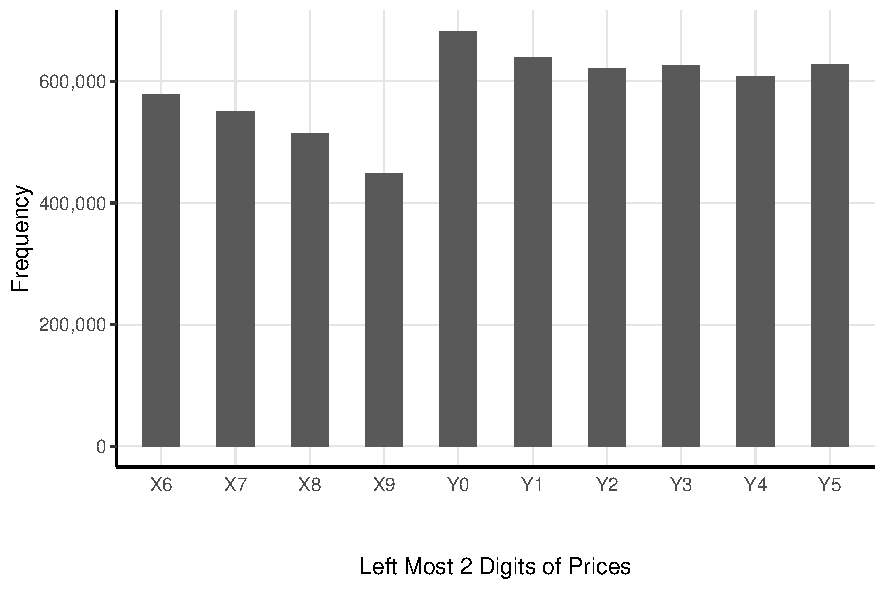
\includegraphics[width=0.65\textwidth]{figures/left2_second_count.pdf}
	\fignote{}
\end{figure}

\begin{figure}[hp]
	\centering%
	\caption{Frequency of Observations for Stocks that Change the First Digit \\ All Stocks (different bin size)}%
	\label{fig:freq_inc}%
	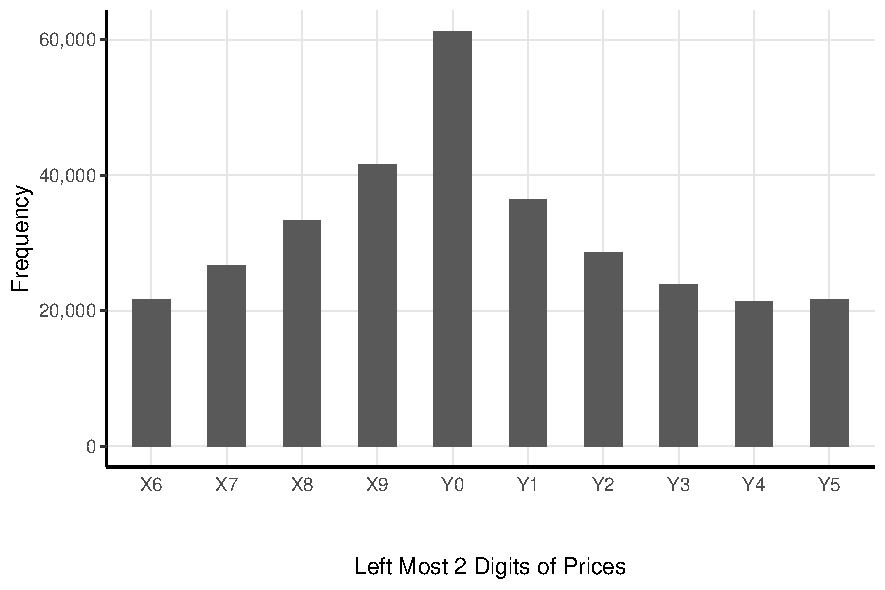
\includegraphics[width=0.65\textwidth]{figures/left2_second_increase_count.pdf}
	\fignote{}
\end{figure}





\begin{figure}[hp]
	\centering%
	\caption{Frequency of Observations  for Stocks that Change the First Digit}%
	\label{fig:freq_inc_samples}%
	\subfigure[Stocks with Prices from £0.11 to £1.01 (1p bins)]{	
		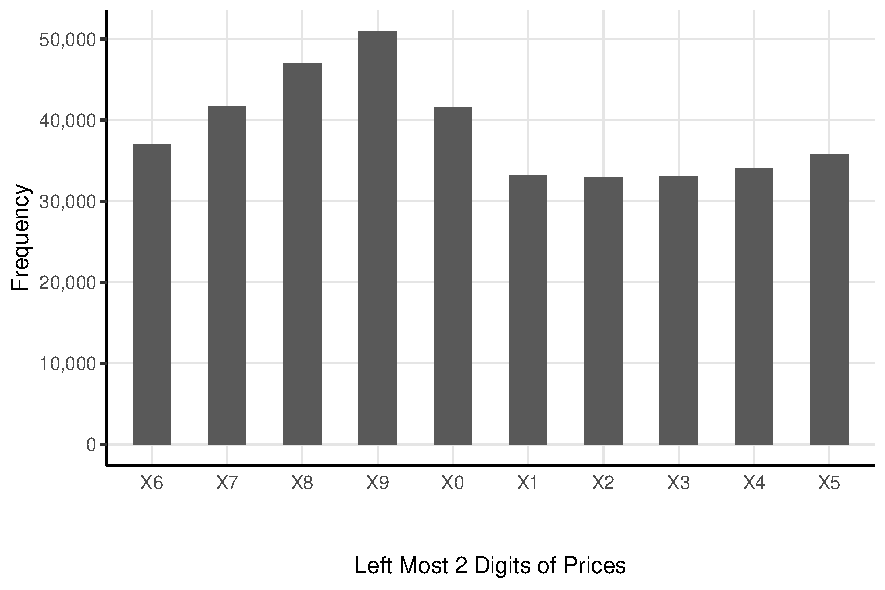
\includegraphics[width=0.65\textwidth]{figures/Left2_second_increases_1pbin_count.pdf}
	}
	\subfigure[Stocks with Prices from £1.1 to £10.1  (10p  bins)]{	
		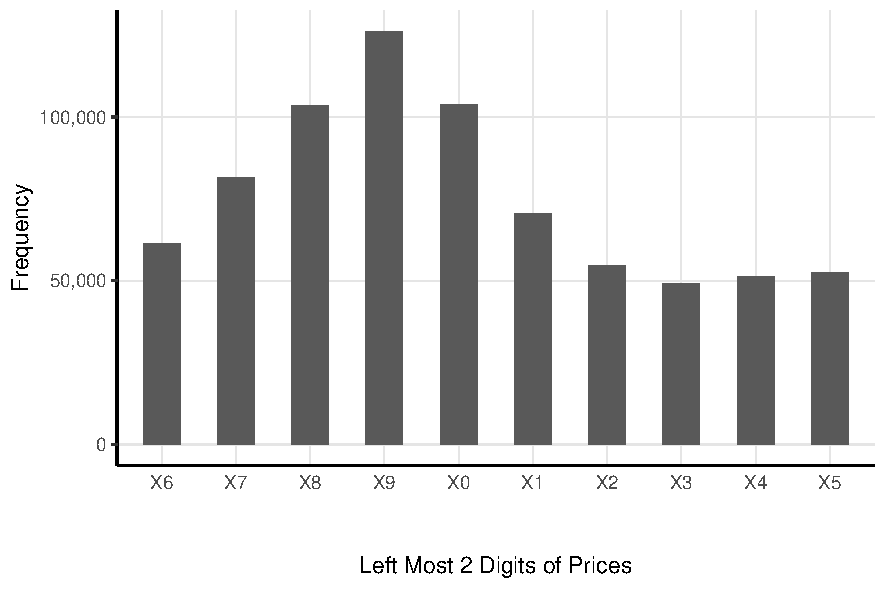
\includegraphics[width=0.65\textwidth]{figures/Left2_second_increases_10pbin_count.pdf}
	}	
	\subfigure[Stocks with Prices from £11 to £101 
	(£1  bins)]{	
		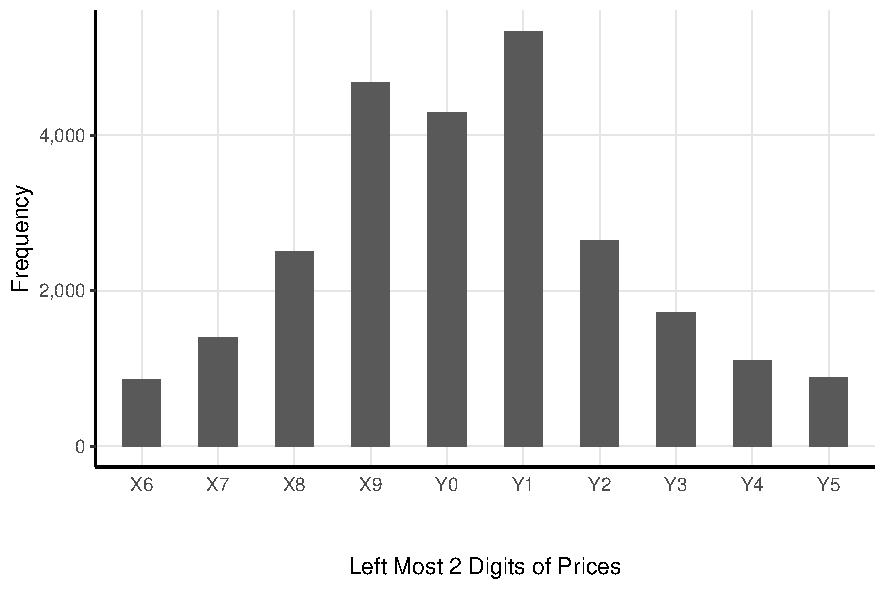
\includegraphics[width=0.65\textwidth]{figures/Left2_second_increases_1poundbin_count.pdf}
	}	
	\fignote{  }
\end{figure}





\clearpage
\subsection{Effect of Left Digits when Prices Decrease}

Here I used the excluded quarters from the sample restriction described in the previous section.

\subsubsection{Raw Patterns Showing the First Two Digits and the Probability to Sell}

\begin{figure}[hbt!]
	\centering%
	\caption{Probability of Selling  for Stocks that Do not Change the First Digit \\ All Stocks (different bin size)}%
	\label{fig:}%
	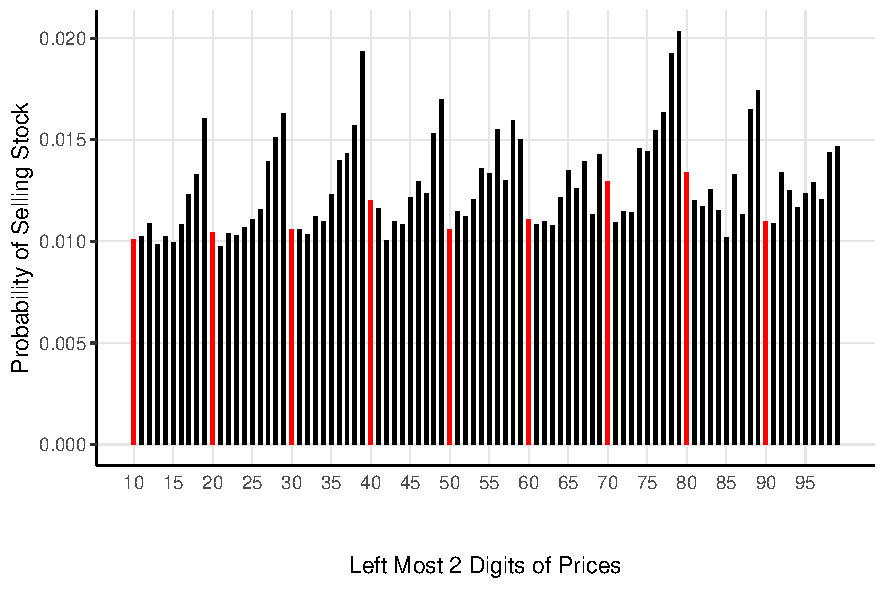
\includegraphics[width=0.65\textwidth]{figures/2left_decrease.pdf}
	\fignote{}
\end{figure}

Note above that the 10 bar is the first one, I put it at the beginning because prices are generally moving down from 11 bar to 10 bar.

Also, note in the next figure that the subsamples are a bit different. For instance, the first subsample goes from £0.10 to less than £1.00 rather than from £0.11 to less than £1.01. This is because the second digit 0 should include prices in the bin £0.10, because we are interested in observing what happen when prices  move down from £0.11 to £0.10 (in the previous analysis prices were, however, moving up from second digit £0.99 to £1.00 and we were interested in observing what happen in the £1.00 bin).

\begin{figure}[hp]
	\centering%
	\caption{Probability of Selling  for Stocks that Do not Change the First Digit}%
	\label{fig:bars_prob}%
	\subfigure[Stocks with Prices from £0.10 to £1.00 (1p bins)]{	
		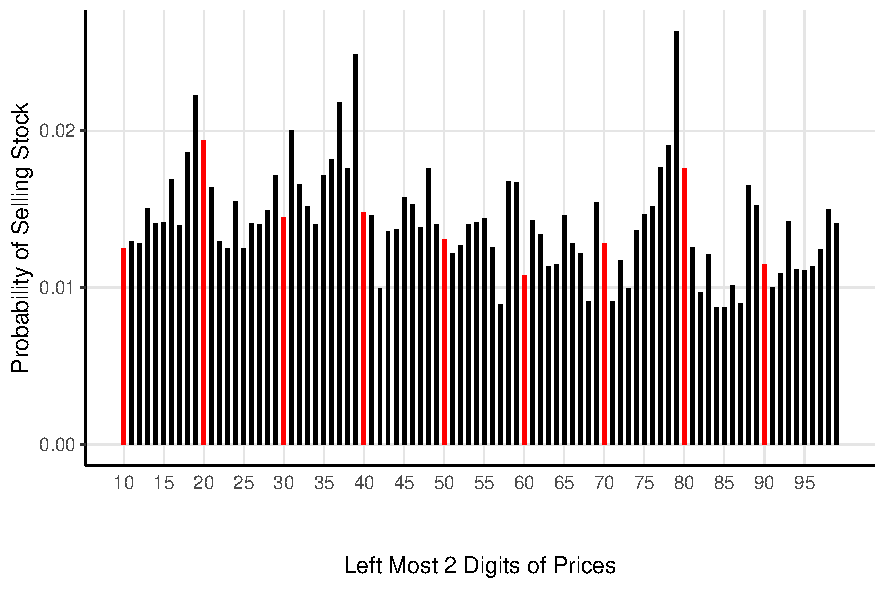
\includegraphics[width=0.65\textwidth]{figures/2left_decrease_bin1p.pdf}
	}
	\subfigure[Stocks with Prices from £1.00 to £10.00  (10p  bins)]{	
		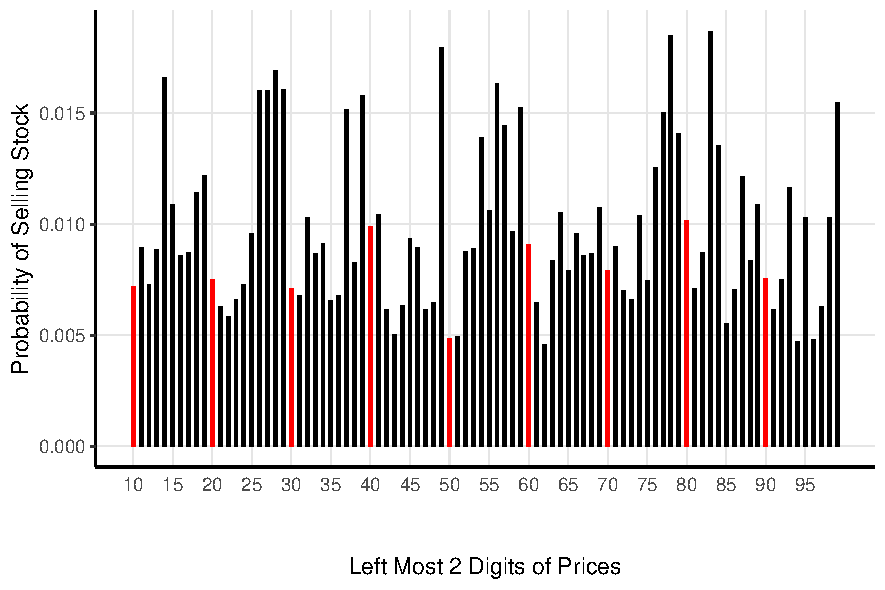
\includegraphics[width=0.65\textwidth]{figures/2left_decrease_bin10p.pdf}
	}	
	\subfigure[Stocks with Prices from £10 to £100 
	(£1  bins)]{	
		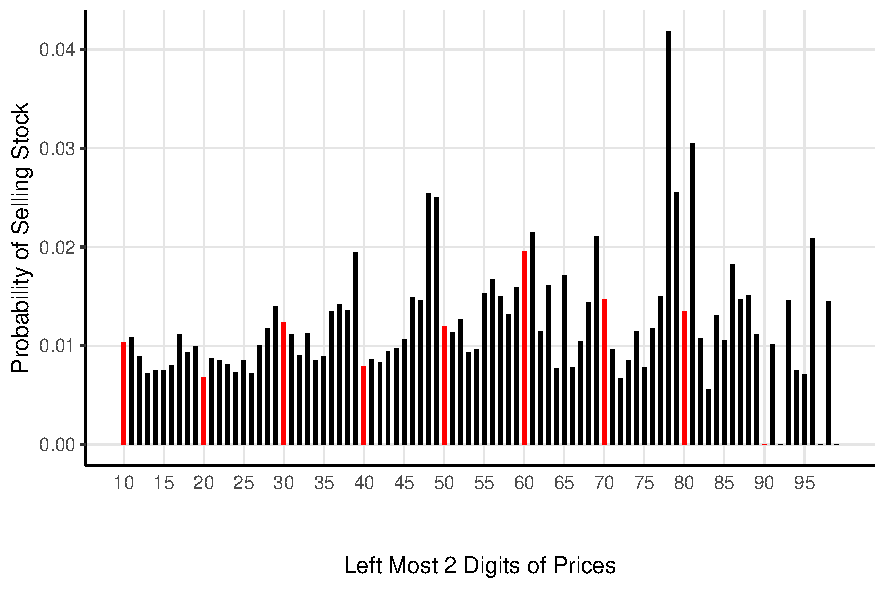
\includegraphics[width=0.65\textwidth]{figures/2left_decrease_bin1pound.pdf}
	}	
	\fignote{  }
\end{figure}

\clearpage
\subsubsection{Raw Patterns Showing the Second Digit and the Probability to Sell}

\begin{figure}[hbt!]
	\centering%
	\caption{Probability of Selling  for Stocks that Do not Change the First Digit \\ All Stocks (different bin size)}%
	\label{fig:prob_all_dec}%
	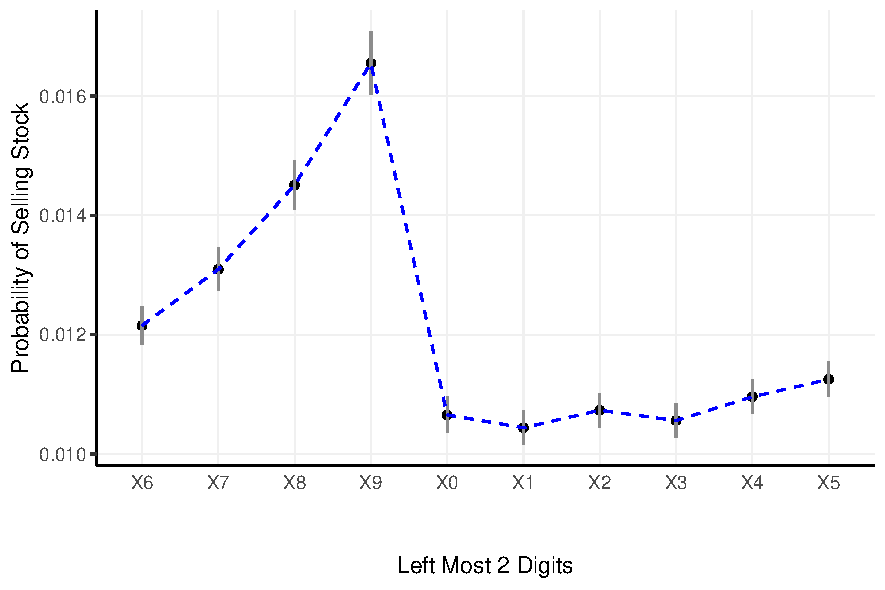
\includegraphics[width=0.65\textwidth]{figures/Left2decrease_probCI.pdf}
	\fignote{}
\end{figure}


\begin{figure}[hp]
	\centering%
	\caption{Probability of Selling  for Stocks that Change Do not the First Digit}%
	\label{fig:prob_all_dec_samples}%
	\subfigure[Stocks with Prices from £0.11 to £1.01 (1p bins)]{	
		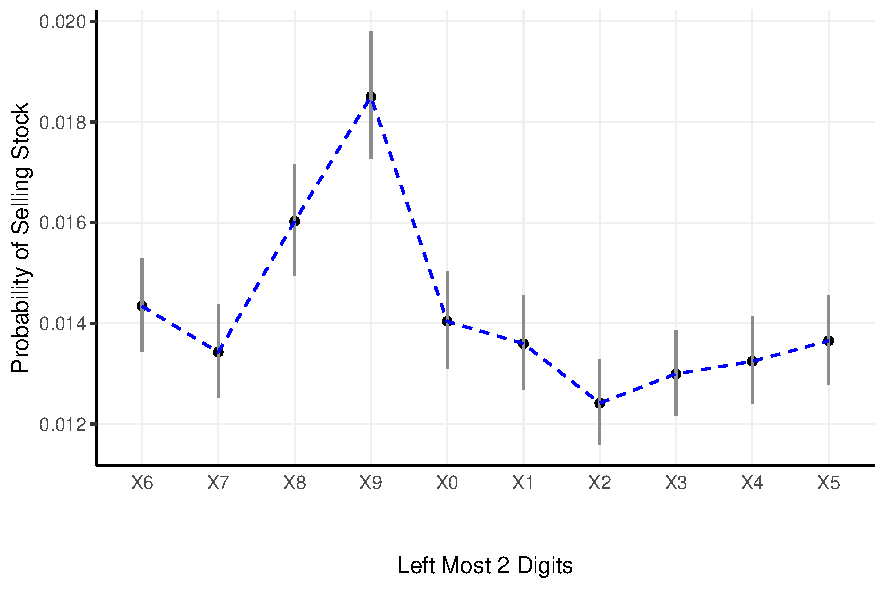
\includegraphics[width=0.65\textwidth]{figures/Left2decreases_1pbin_CI.pdf}
	}
	\subfigure[Stocks with Prices from £1.1 to £10.1  (10p  bins)]{	
		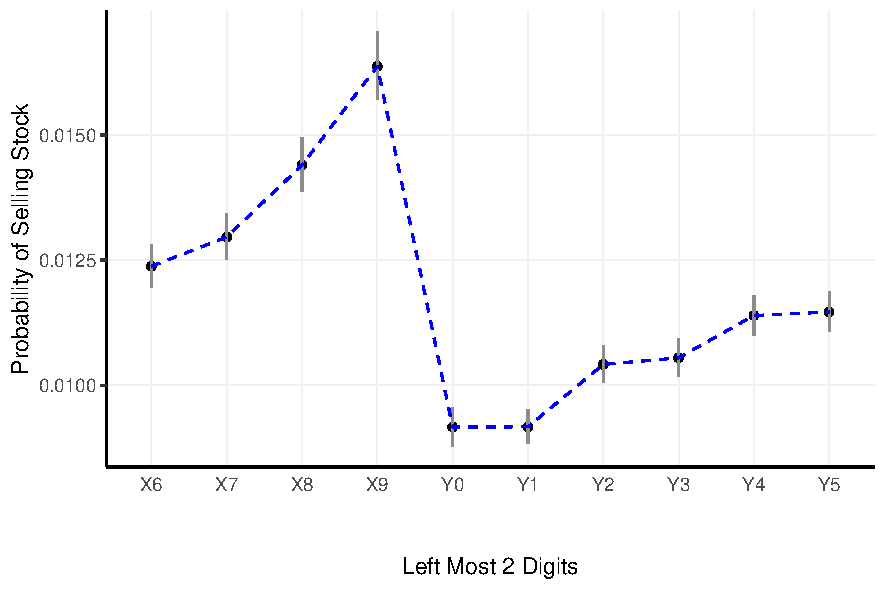
\includegraphics[width=0.65\textwidth]{figures/Left2decreases_10pbin_CI.pdf}
	}	
	\subfigure[Stocks with Prices from £11 to £101 
	(£1  bins)]{	
		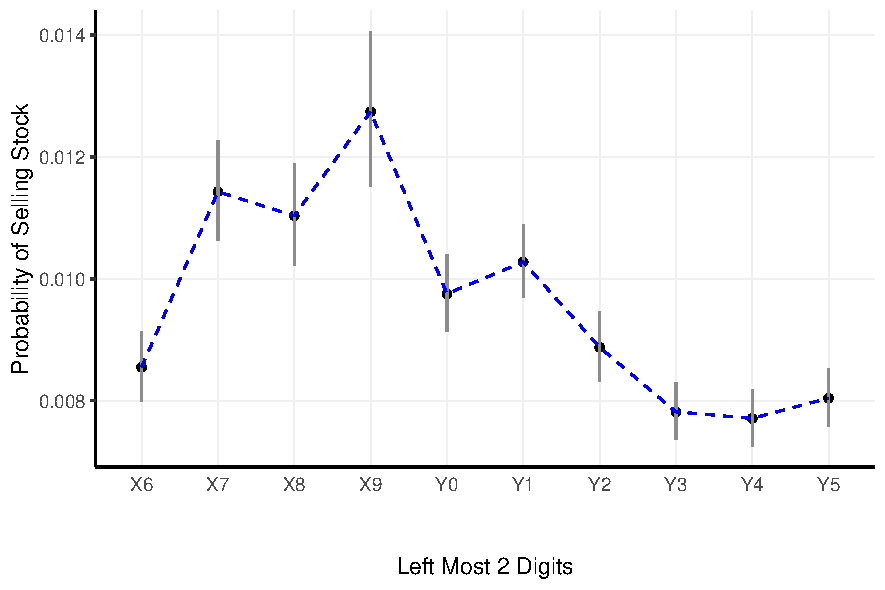
\includegraphics[width=0.65\textwidth]{figures/Left2decreases_1poundbin_CI.pdf}
	}	
	\fignote{  }
\end{figure}

\clearpage


\clearpage
\subsection{Regressions}

\begin{econtable}[h]\footnotesize
	\caption{All Stocks}
	\label{tab:}
	\estauto{l c c c c c c  }{
		& \multicolumn{5}{c}{$Probability\:  of\:  Sale_{ijt}=1$} \\ 
		%	\cmidrule(rr){2-7}
		& \multicolumn{1}{c}{(1)} & \multicolumn{1}{c}{(2)} & \multicolumn{1}{c}{(3)} & \multicolumn{1}{c}{(4)} & 
		\multicolumn{1}{c}{(5)} & \\ 
		\midrule
		\\[-2.1ex] Second Digit Over Threshold = 1 (in Range X0 to X5) & -0.0029{***} & -0.0057{***} & -0.0056{***} & -0.0054{***} & -0.0057{***} \\ 
  & (0.0001) & (0.0003) & (0.0003) & (0.0003) & (0.0003) \\ 
  Second Digit Over Threshold (= 0 to 5, corresponding to X0 to X5) &  & 0.0001{***} & 0.0002{***} & 0.0004{***} & 0.0004{***} \\ 
  &  & (0.0000) & (0.0000) & (0.0000) & (0.0000) \\ 
  Second Digit Below Threshold (= -3 to 0, corresponding to X6 to X9) &  & 0.0014{***} & 0.0013{***} & 0.0011{***} & 0.0011{***} \\ 
  &  & (0.0001) & (0.0001) & (0.0001) & (0.0001) \\ 
  Constant & 0.0137{***} & 0.0162{***} & 0.0193{***} &  &  \\ 
  & (0.0003) & (0.0004) & (0.0019) &  &  \\ 
 Day FE & NO & NO & YES & YES & YES \\ 
Industry FE & NO & NO & YES & YES & YES \\ 
Account FE & NO & NO & NO & YES & YES \\ 
Stock FE & NO & NO & NO & NO & YES \\ 
Observations & \multicolumn{1}{c}{4,376,352} & \multicolumn{1}{c}{4,376,352} & \multicolumn{1}{c}{4,376,352} & \multicolumn{1}{c}{4,376,352} & \multicolumn{1}{c}{4,376,352} \\ 
R$^{2}$ & \multicolumn{1}{c}{0.0002} & \multicolumn{1}{c}{0.0002} & \multicolumn{1}{c}{0.0009} & \multicolumn{1}{c}{0.0492} & \multicolumn{1}{c}{0.0526} \\ 
 
	}
	\fignote{The unit of observation is an investor $\times$ stock $\times$ day. The samples is restricted to login days. We include only quarters in which the stocks have not increased in price (regarding the first observation of the quarter) and have not changed the left most digit at least once during the quarter. Regressions fit an intercept for the change in the left most digit at X0 and two slopes for the left (X6 to X9) and right (X0 to X5) values, as described by the raw patterns in \ref{fig:prob_all_dec}. The constant shows the probability to sell the stock at when the second digit is 9 (X9). The second digit over threshold dummy shows the jump in probability when the first digit changes and so the second digit becomes 0 (X0). SE are clustered by account.}
\end{econtable}


\begin{econtable}[h]\footnotesize
	\caption{Stocks with Prices Between \pounds 0.10 to \pounds 1.0 }
	\label{tab:}
	\estauto{l c c c c c c  }{
		& \multicolumn{5}{c}{$Probability\:  of\:  Sale_{ijt}=1$} \\ 
		%	\cmidrule(rr){2-7}
		& \multicolumn{1}{c}{(1)} & \multicolumn{1}{c}{(2)} & \multicolumn{1}{c}{(3)} & \multicolumn{1}{c}{(4)} & 
		\multicolumn{1}{c}{(5)} & \\ 
		\midrule
		 Above Y0 = 1 (in Range Y0 to Y5) & -0.0035{***} & -0.0045{***} & -0.0051{***} & -0.0048{***} & -0.0052{***} \\ 
  & (0.0008) & (0.0012) & (0.0012) & (0.0012) & (0.0013) \\ 
  Stock Digits Y0 to Y5 &  & -0.0004{*} & -0.0003 & 0.0001 & 0.0002 \\ 
  &  & (0.0003) & (0.0003) & (0.0003) & (0.0003) \\ 
  Stock Digits X6 to X9 &  & 0.0015{***} & 0.0015{***} & 0.0011{**} & 0.0012{**} \\ 
  &  & (0.0005) & (0.0005) & (0.0005) & (0.0005) \\ 
  Constant & 0.0147{***} & 0.0167{***} & 0.0613{**} &  &  \\ 
  & (0.0008) & (0.0011) & (0.0291) &  &  \\ 
 Day FE & NO & NO & YES & YES & YES \\ 
Industry FE & NO & NO & YES & YES & YES \\ 
Account FE & NO & NO & NO & YES & YES \\ 
Stock FE & NO & NO & NO & NO & YES \\ 
Observations & \multicolumn{1}{c}{114,133} & \multicolumn{1}{c}{114,133} & \multicolumn{1}{c}{114,133} & \multicolumn{1}{c}{114,133} & \multicolumn{1}{c}{114,133} \\ 
R$^{2}$ & \multicolumn{1}{c}{0.0002} & \multicolumn{1}{c}{0.0003} & \multicolumn{1}{c}{0.0015} & \multicolumn{1}{c}{0.1445} & \multicolumn{1}{c}{0.1599} \\ 
 
	}
	\fignote{The unit of observation is an investor $\times$ stock $\times$ day. The samples is restricted to login days. We include only quarters in which the stocks have not increased in price (regarding the first observation of the quarter) and have not changed the left most digit at least once during the quarter. Regressions fit an intercept for the change in the left most digit at X0 and two slopes for the left (X6 to X9) and right (X0 to X5) values, as described by the raw patterns in \ref{fig:prob_all_dec_samples}. The constant shows the probability to sell the stock at when the second digit is 9 (X9). The second digit over threshold dummy shows the jump in probability when the first digit changes and so the second digit becomes 0 (X0). SE are clustered by account.}
\end{econtable}


\begin{econtable}[h]\footnotesize
	\caption{Stocks with Prices Between \pounds 1 to \pounds 10}
	\label{tab:}
	\estauto{l c c c c c c  }{
		& \multicolumn{5}{c}{$Probability\:  of\:  Sale_{ijt}=1$} \\ 
		%	\cmidrule(rr){2-7}
		& \multicolumn{1}{c}{(1)} & \multicolumn{1}{c}{(2)} & \multicolumn{1}{c}{(3)} & \multicolumn{1}{c}{(4)} & 
		\multicolumn{1}{c}{(5)} & \\ 
		\midrule
		\\[-2.1ex] Second Digit Over Threshold = 1 (in Range X0 to X5) & -0.0033{***} & -0.0069{***} & -0.0065{***} & -0.0063{***} & -0.0068{***} \\ 
  & (0.0002) & (0.0004) & (0.0004) & (0.0004) & (0.0004) \\ 
  Second Digit Over Threshold (= 0 to 5, corresponding to X0 to X5) &  & 0.0005{***} & 0.0004{***} & 0.0004{***} & 0.0005{***} \\ 
  &  & (0.0001) & (0.0001) & (0.0001) & (0.0001) \\ 
  Second Digit Below Threshold (= -3 to 0, corresponding to X6 to X9) &  & 0.0013{***} & 0.0012{***} & 0.0012{***} & 0.0011{***} \\ 
  &  & (0.0001) & (0.0001) & (0.0001) & (0.0001) \\ 
  Constant & 0.0137{***} & 0.0159{***} & 0.0256{***} &  &  \\ 
  & (0.0004) & (0.0005) & (0.0014) &  &  \\ 
 Day FE & NO & NO & YES & YES & YES \\ 
Industry FE & NO & NO & YES & YES & YES \\ 
Account FE & NO & NO & NO & YES & YES \\ 
Stock FE & NO & NO & NO & NO & YES \\ 
Observations & \multicolumn{1}{c}{2,461,228} & \multicolumn{1}{c}{2,461,228} & \multicolumn{1}{c}{2,461,228} & \multicolumn{1}{c}{2,461,228} & \multicolumn{1}{c}{2,461,228} \\ 
R$^{2}$ & \multicolumn{1}{c}{0.0002} & \multicolumn{1}{c}{0.0003} & \multicolumn{1}{c}{0.0011} & \multicolumn{1}{c}{0.0551} & \multicolumn{1}{c}{0.0572} \\ 
 
	}
	\fignote{The unit of observation is an investor $\times$ stock $\times$ day. The samples is restricted to login days. We include only quarters in which the stocks have not increased in price (regarding the first observation of the quarter) and have not changed the left most digit at least once during the quarter.  Regressions fit an intercept for the change in the left most digit at X0 and two slopes for the left (X6 to X9) and right (X0 to X5) values, as described by the raw patterns in \ref{fig:prob_all_dec_samples}. The constant shows the probability to sell the stock at when the second digit is 9 (X9). The second digit over threshold dummy shows the jump in probability when the first digit changes and so the second digit becomes 0 (X0). SE are clustered by account.}
\end{econtable}

\begin{econtable}[h]\footnotesize
	\caption{Stocks with Prices Between \pounds 10 to \pounds 100}
	\label{tab:}
	\estauto{l c c c c c c  }{
		& \multicolumn{5}{c}{$Probability\:  of\:  Sale_{ijt}=1$} \\ 
		%	\cmidrule(rr){2-7}
		& \multicolumn{1}{c}{(1)} & \multicolumn{1}{c}{(2)} & \multicolumn{1}{c}{(3)} & \multicolumn{1}{c}{(4)} & 
		\multicolumn{1}{c}{(5)} & \\ 
		\midrule
		\\[-2.1ex] Second Digit Over Threshold = 1 (in Range X0 to X5) & -0.0017{***} & -0.0029{***} & -0.0029{***} & -0.0047{***} & -0.0057{***} \\ 
  & (0.0003) & (0.0006) & (0.0006) & (0.0006) & (0.0007) \\ 
  Second Digit Over Threshold (= 0 to 5, corresponding to X0 to X5) &  & -0.0005{***} & -0.0003{***} & 0.0001{*} & 0.0003{***} \\ 
  &  & (0.0001) & (0.0001) & (0.0001) & (0.0001) \\ 
  Second Digit Below Threshold (= -3 to 0, corresponding to X6 to X9) &  & 0.0013{***} & 0.0012{***} & 0.0011{***} & 0.0012{***} \\ 
  &  & (0.0002) & (0.0002) & (0.0002) & (0.0002) \\ 
  Constant & 0.0104{***} & 0.0129{***} & 0.0146{***} &  &  \\ 
  & (0.0004) & (0.0007) & (0.0010) &  &  \\ 
 Day FE & NO & NO & YES & YES & YES \\ 
Industry FE & NO & NO & YES & YES & YES \\ 
Account FE & NO & NO & NO & YES & YES \\ 
Stock FE & NO & NO & NO & NO & YES \\ 
Observations & \multicolumn{1}{c}{978,415} & \multicolumn{1}{c}{978,415} & \multicolumn{1}{c}{978,415} & \multicolumn{1}{c}{978,415} & \multicolumn{1}{c}{978,415} \\ 
R$^{2}$ & \multicolumn{1}{c}{0.0001} & \multicolumn{1}{c}{0.0002} & \multicolumn{1}{c}{0.0006} & \multicolumn{1}{c}{0.0607} & \multicolumn{1}{c}{0.0641} \\ 
 
	}
	\fignote{The unit of observation is an investor $\times$ stock $\times$ day. The samples is restricted to login days. We include only quarters in which the stocks have not increased in price (regarding the first observation of the quarter) and have not changed the left most digit at least once during the quarter.  Regressions fit an intercept for the change in the left most digit at X0 and two slopes for the left (X6 to X9) and right (X0 to X5) values, as described by the raw patterns in \ref{fig:prob_all_dec_samples}. The constant shows the probability to sell the stock at when the second digit is 9 (X9). The second digit over threshold dummy shows the jump in probability when the first digit changes and so the second digit becomes 0 (X0). SE are clustered by account.}
\end{econtable}

\clearpage

\subsubsection{Frequency of Observations in the Samples}

We might show plots with the frequency of observations in an appendix.

\begin{figure}[h]
	\centering%
	\caption{Frequency of Observations for Stocks that Change the First Digit \\ All Stocks (different bin size)}%
	\label{fig:}%
	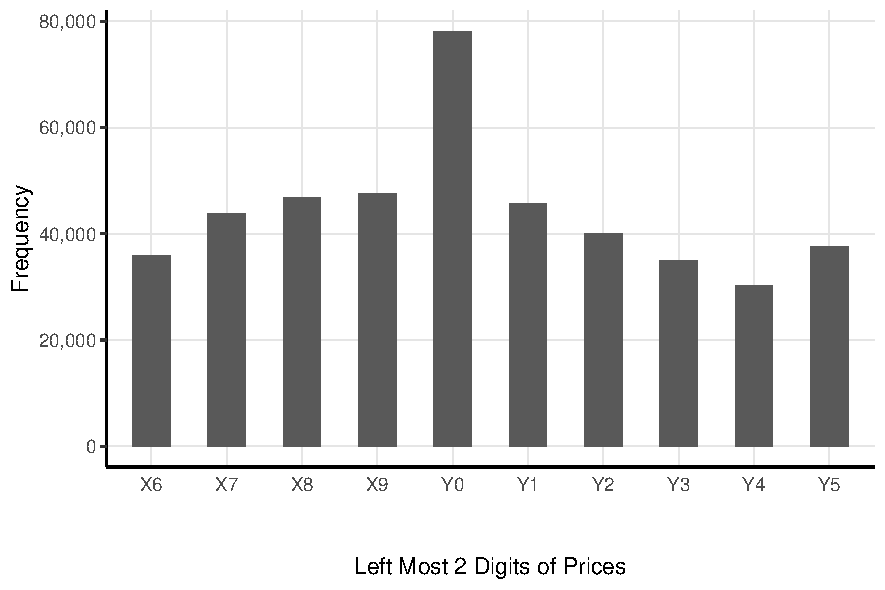
\includegraphics[width=0.65\textwidth]{figures/left2_second_decrease_count.pdf}
	\fignote{}
\end{figure}





\begin{figure}[hp]
	\centering%
	\caption{Frequency of Observations  for Stocks that Change the First Digit}%
	\label{fig:}%
	\subfigure[Stocks with Prices from £0.11 to £1.01 (1p bins)]{	
		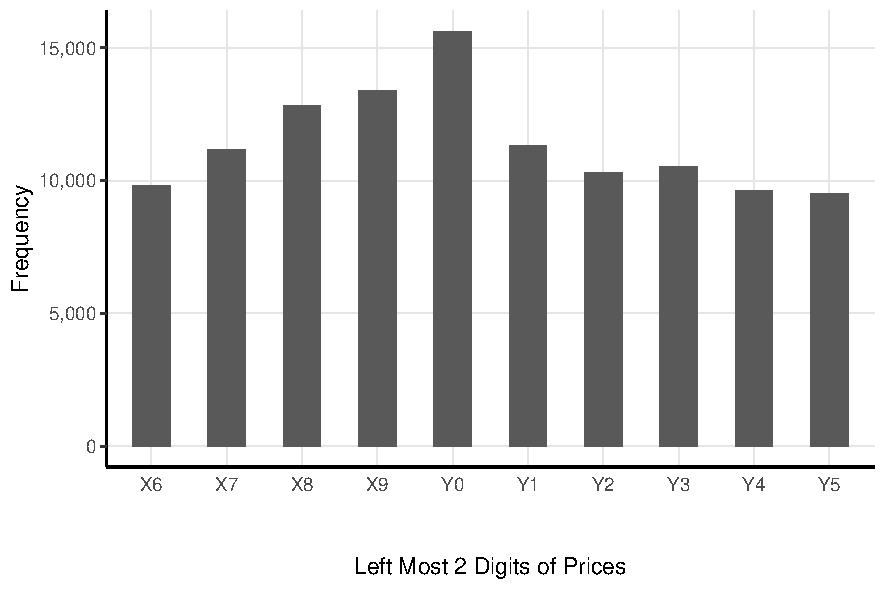
\includegraphics[width=0.65\textwidth]{figures/Left2_second_decreases_1pbin_count.pdf}
	}
	\subfigure[Stocks with Prices from £1.1 to £10.1  (10p  bins)]{	
		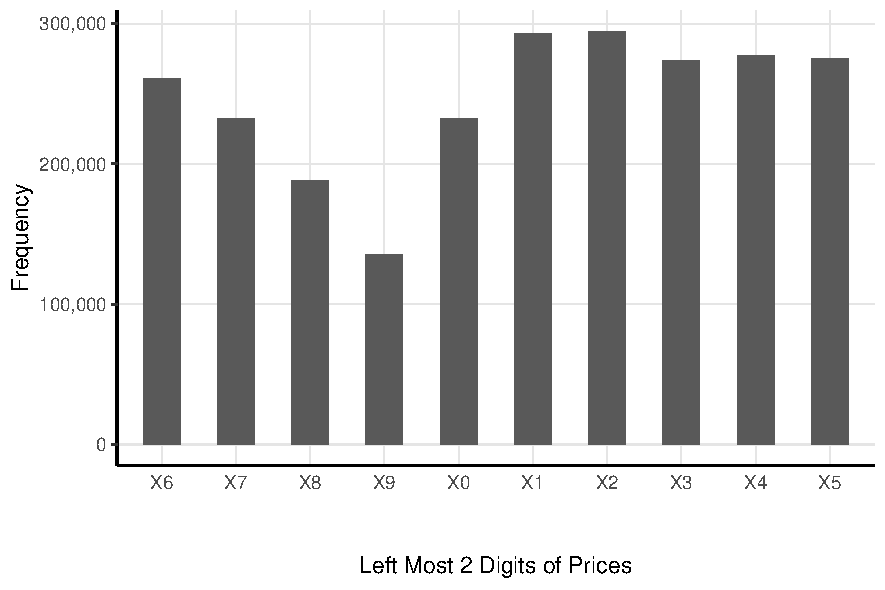
\includegraphics[width=0.65\textwidth]{figures/Left2_second_decreases_10pbin_count.pdf}
	}	
	\subfigure[Stocks with Prices from £11 to £101 
	(£1  bins)]{	
		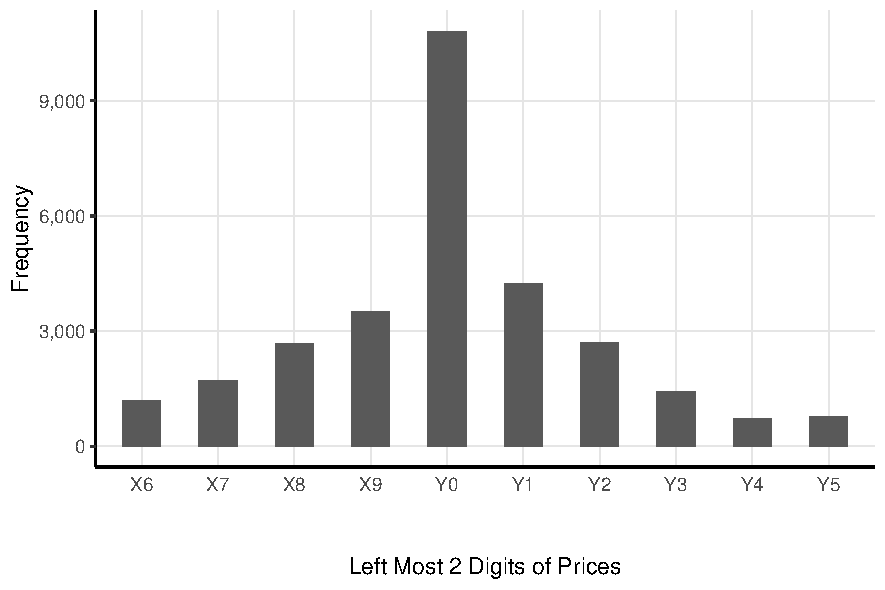
\includegraphics[width=0.65\textwidth]{figures/Left2_second_decreases_1poundbin_count.pdf}
	}	
	\fignote{  }
\end{figure}




\clearpage
\subsection{Sell days with no login}

\textcolor{blue}{\textbf{UPDATE: after our last discussion, it is enough to look at the raw probabilities that are large when the second digit is either 9 or 1 to show that our results are not driven by limit orders. The analysis of sell days with no logins is unnecessary and it actually did not work because of the few number of observations.}}

Unfortunately, we cannot distinguish limit orders in the data. The narratives of the transactions have not enough information to allow us to identify limit orders. Here I am looking at those days in which there were sells with no login into the account. These days are more likely to show the execution of limit orders. If we cannot identify the effect of a change in the left most digit, then limit orders are not a problem for our estimation. 
However, after looking into the data, we have a very tiny sample to do this analysis.

 We have 1669  accounts with sells in days with no logins (22595 observations, account $\times$ stock $\times$ day), but for consistency we have to use the observations for the quarters in which the price increase and change the first digit. This restriction leave us with a subset of 6713 observations.
This is a very tiny proportion compared to the number of observations from the previous analysis (login days, including quarter in which the price goes up and there is a change in the left digit: 1517823 observations).


I used the remaining 15882 observations to see the patterns for quarters when prices move down (even if the left digit has not changed, like in the previous analysis). 

The patterns do not make apparent the effect of a change in the left most digit. But I think we cannot say much because the number of observations is tiny. Any thoughts on how to address in the paper the fact that we cannot distinguish limit orders?


\begin{figure}[hp]
	\centering%
	\caption{Probability of Selling for Sell Days with no Logins}%
	\label{fig:bars_prob}%
	\subfigure[Stocks with Prices that Increase and Change Left Digit]{	
		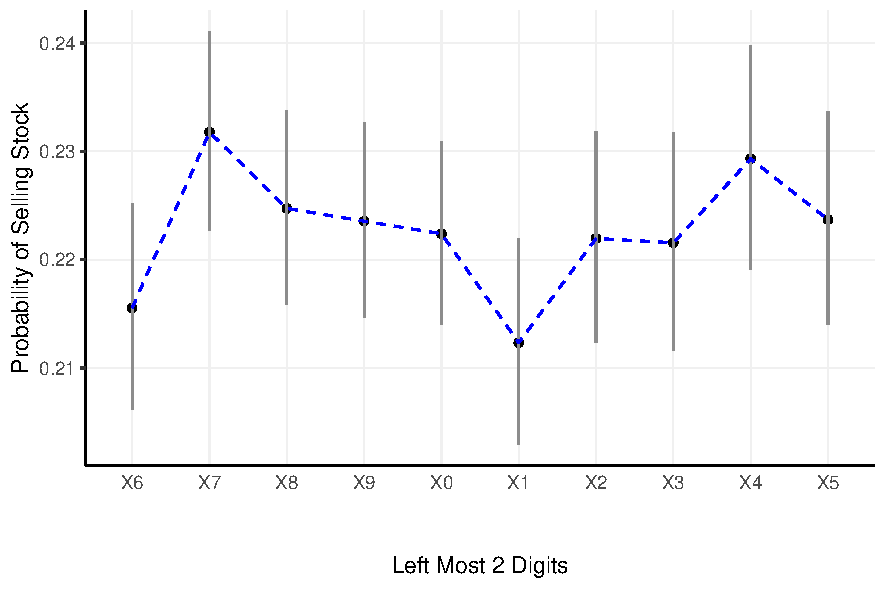
\includegraphics[width=0.65\textwidth]{figures/Left2increase_sell_no_login.pdf}
	}
	\subfigure[All the Other Stocs and Quarters]{	
		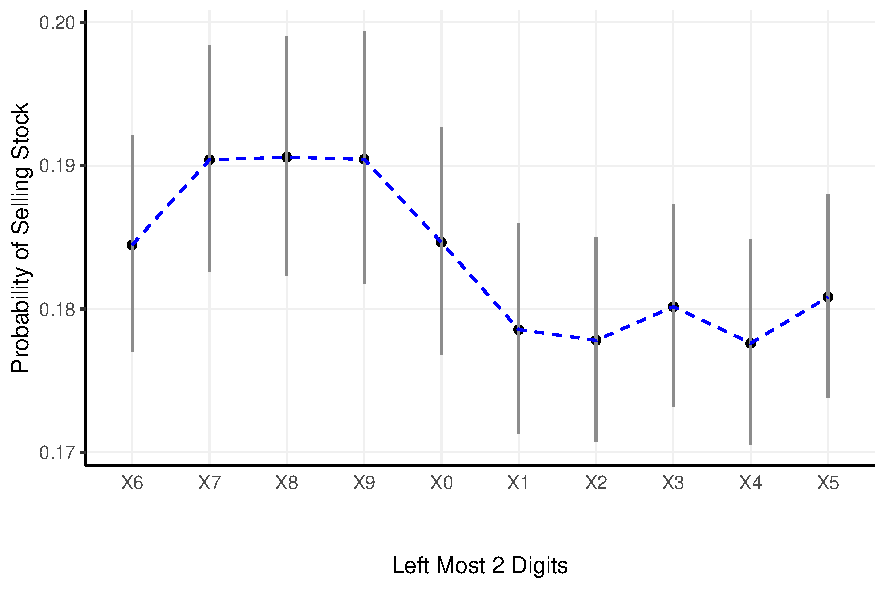
\includegraphics[width=0.65\textwidth]{figures/Left2decrease_sell_no_login.pdf}
	}		
	\fignote{  }
\end{figure}


\clearpage


\subsection{Changes in the Second Left Most Digit}

Now we will explore whether the changes in the second left most digit might have an effect in the probability to sell. We will analyse how the probabilities to sell change when the third digit becomes zero.

For convenience, I use the sample sample of quarters in which prices change the first digit. If they change the first digit, they should have changed the second digit too. There are not clear patterns. Even when I look at subsamples in \ref{fig:bars_probthird}.

\begin{landscape}

\subsubsection{Raw Patterns Showing the First Three Digits and the Probability to Sell}

\begin{figure}[hbt!]
	\centering%
	\caption{Probability of Selling  for Stocks that Change the First Digit \\ All Stocks (different bin size)}%
	\label{fig:all_obs}%
	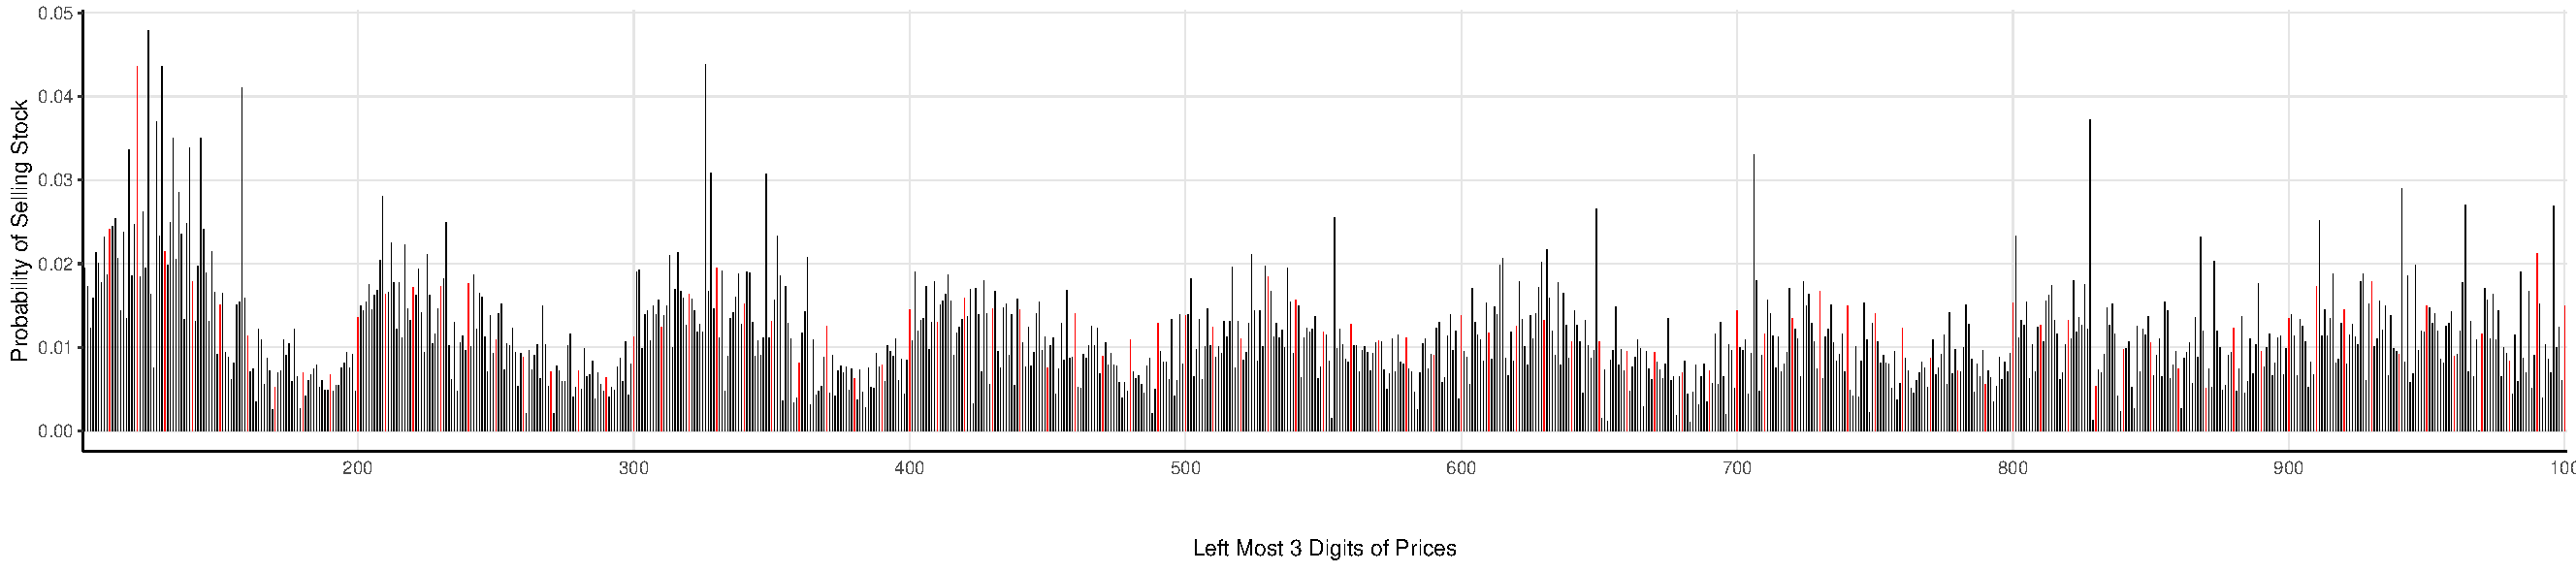
\includegraphics[width=1.6\textwidth]{figures/3left_increase.pdf}
	\fignote{}
\end{figure}
\end{landscape}

\clearpage
\subsubsection{Raw Patterns Showing the Third Digit and the Probability to Sell}

\begin{figure}[hbt!]
	\centering%
	\caption{Probability of Selling  for Stocks that Change the First Digit \\ All Stocks (different bin size)}%
	\label{fig:}%
	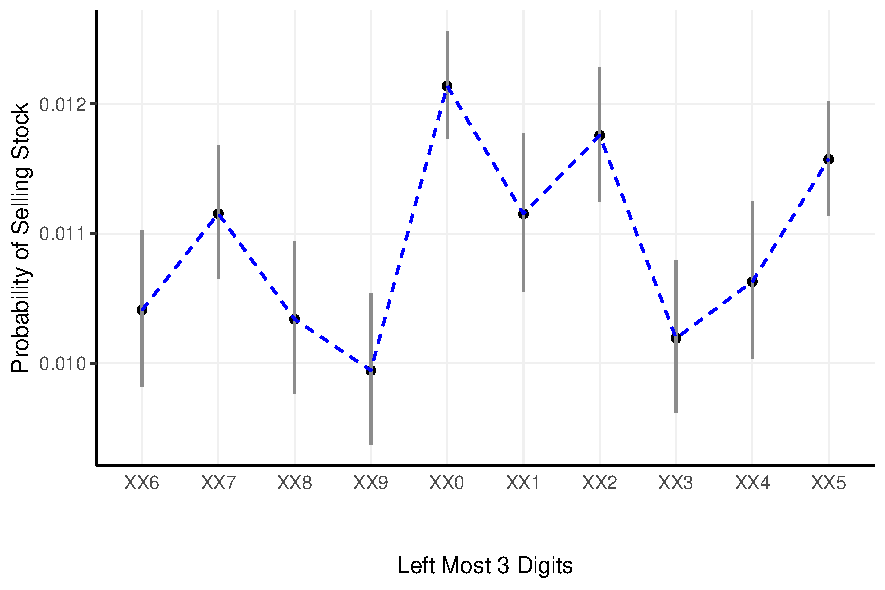
\includegraphics[width=0.65\textwidth]{figures/Left3increase_probCI.pdf}
	\fignote{}
\end{figure}


\begin{figure}[hp]
	\centering%
	\caption{Probability of Selling  for Stocks that Change the First Digit}%
	\label{fig:bars_probthird}%
	\subfigure[Stocks with Prices from £1.01 to £10.01 (1p bins)]{	
		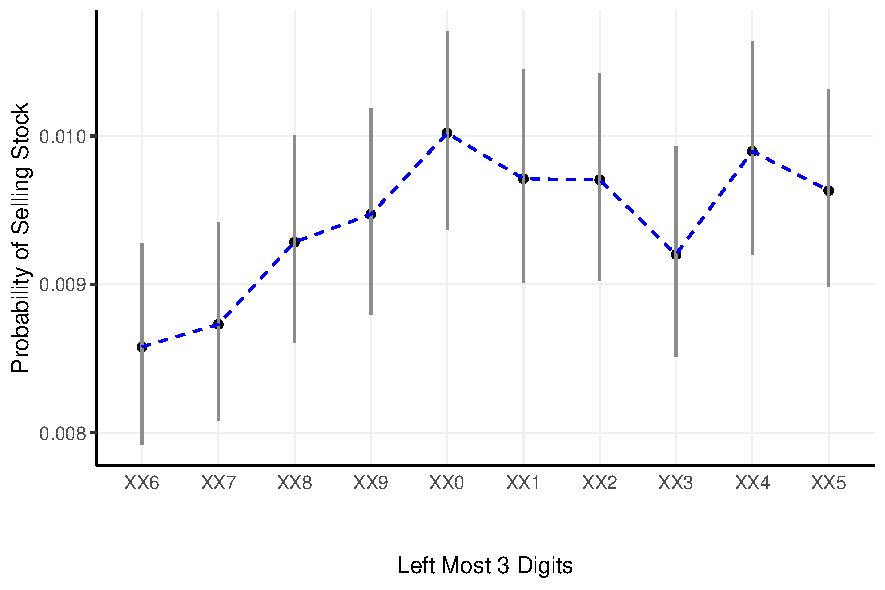
\includegraphics[width=0.65\textwidth]{figures/Left3increases_1pbin_CI.pdf}
	}
	\subfigure[Stocks with Prices from £10.1 to £100.1  (10p  bins)]{	
		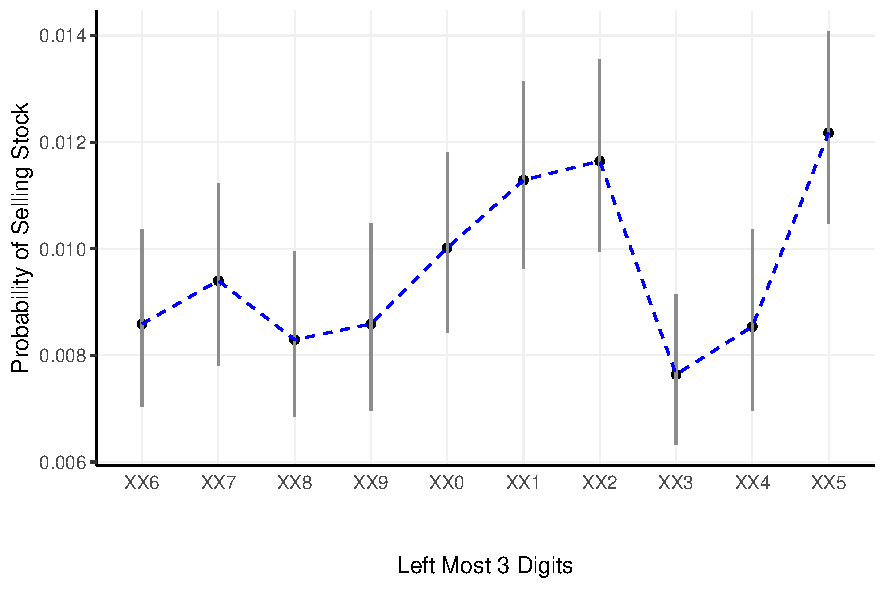
\includegraphics[width=0.65\textwidth]{figures/Left3increases_10pbin_CI.pdf}
	}		
	\fignote{  }
\end{figure}



\clearpage
\section{Selling patterns when the peak price is the highest price experienced by the investor}

\subsection{Definition of Peak Prices}
I have used four definitions of peak values. 

\begin{itemize}
	\item Case 1: The peak value is the highest price since the purchase day (there are no restrictions on how much prices decline after the peak day). The only requirement is that the day before (and the day after) the peak day the price have to be smaller than during the peak day. In this case, if an stock has crossed a peak price yesterday, the price yesterday could become a new peak price tomorrow if today the price has gone down.
	
	Because in Case 1, there are many new peak prices every time the stock crosses a peak value and goes down a bit, Cases 2, 3 and 4 add the restriction that a peak price has to be the highest price for some interval of time.
	
	\item Case 2: The potential peak value has to be the highest price for at least a week to be considerer a peak price.
	\item  Case 3: The potential peak value has to be the highest price for at least a month to be considerer a peak price.
	\item  Case 4: The potential peak value has to be the highest price for at least a quarter to be considerer a peak price.	
	
\end{itemize}


Cases 2 to 4 are not as restrictive as my earlier requirement of a decline in 5\% in prices after the peak day---because they allow to identify a higher number of peaks. 

\ref{fig:example_peak} shows the peak values under these four cases. Cases 2, 3 and 4 are compared against Case 1. In Panel A we compare cases 1 and 2, all points (green and blue) are peak values in Case 1. But the green points are only peak values for Case 2. So under Case 1, we have about 20 peak days (green and blue points in panel A); but under Case 2, we have only 12 peak days (green points in panel A). Panel B compares cases 1 and 3. There is only one peak day in Case 3 (green point in panel B). Panel C compares cases 1 and 4. There are no peak days in Case 4 (no green points in panel C).

\subsection{Disposition Effect Since Latest Peak Price Day}

\ref{fig:DE_peak} shows the DE since peak price for each case. In all cases there is a jump when investor is in gain since latest peak price. For cases 2 to 4, the jump does not always happen at zero returns, probably because people have a different peak value in memory since peak days are not that recent (or maybe people have a rounded value of the peak price in mind).

\subsection{Interaction Between DE Since Peak Price Day and DE Since Purchase Day}
\ref{fig:DE_peak_purc} shows the interaction between the DE since purchase day and the DE since latest peak price day. In Panel A, when investors are in gain since purchase, a gain since the peak price day increases the probability to sell the stock dramatically. This jump is smaller for cases 2, 3 and 4. But the magnitude of the jump is a result of how we defined peak prices.


\subsubsection{Why the effect of a gain since peak day is smaller in cases 2 to 4?}

When there are stronger restrictions to define a peak price, such as in  \textbf{Case 4} requiring that a price to be a peak price has to remain as the highest price for at least a quarter:

\begin{itemize}
	\item The number of peak values is smaller and so the number of observations crossing a peak price before reaching a new (larger) peak price is larger than in Case 1 (i.e., we have a large number of observations with  \textit{gain since peak = 1}). \ref{fig:hist_return_peak} shows the histograms of returns since peak prices for cases 1 and 4.
	
	\item For stocks that have a tendency to be up, the occurrence  of a \textit{gain since peak = 1} is more frequent because these stocks do not update peak values quickly (recall  in Case 4 a peak has to be the highest price for at least one quarter)
	\item  Although in Case 4 the probability to be in gain since peak is larger than in Case 1, the probability to sell an stock in gain since the peak price day should not be necessarily smaller. But it is smaller because people sell stocks the first weeks after crossing the peak value and if they have not done so the first weeks after crossing the peak value, they stick to their choice and do not sell afterwards.	
	
\end{itemize}

The same arguments explain the differences in the interaction between the DE since purchase and since the peak day for Cases 2 and 3.

 \textcolor{blue}{It is clear that there is a DE since peak price day. But to study the interaction between the DE since purchase and since peak price day, we need to decide which definition of peak prices to use. \\
Case 1 shows that the effect of a gain since the peak day is extremely large when peak prices are \textbf{very recent}. This effect is not driven by the effect of gains since latest login, because even though in Case 1 60\% of the peak days were login days, when investors are in \textit{gain since peak=1} only 3\% of the peak days are also the latest login days. \\
Case 4 shows a small effect of gains since peak day because the sells happened during the first days after crossing the peak prices. In Case 4, the median investor (after crossing a peak value) is in \textit{gain since peak=1} for about 39 days. But 50\% of the sales happened just during the first two weeks after crossing the peak value. This is quite different from Case 1 because there the median investor is in \textit{gain since peak=1} for just one day and 50\% of the sales happened just the day when the price crossed the peak value. \\
So to study the DE since peak day, I think that we need to control for how many days the stock has been in gain since the peak day and of course decide which definition of peak prices to use.}
 




\begin{figure}%
	\centering%
	\caption{Example Peak Prices  \\
	Comparison of Peak Prices for Cases 2, 3 and 4 against Case 1}%
	\label{fig:example_peak}%
	\subfigure[Case 2: Peak has to be the highest price for at least a week]{	
		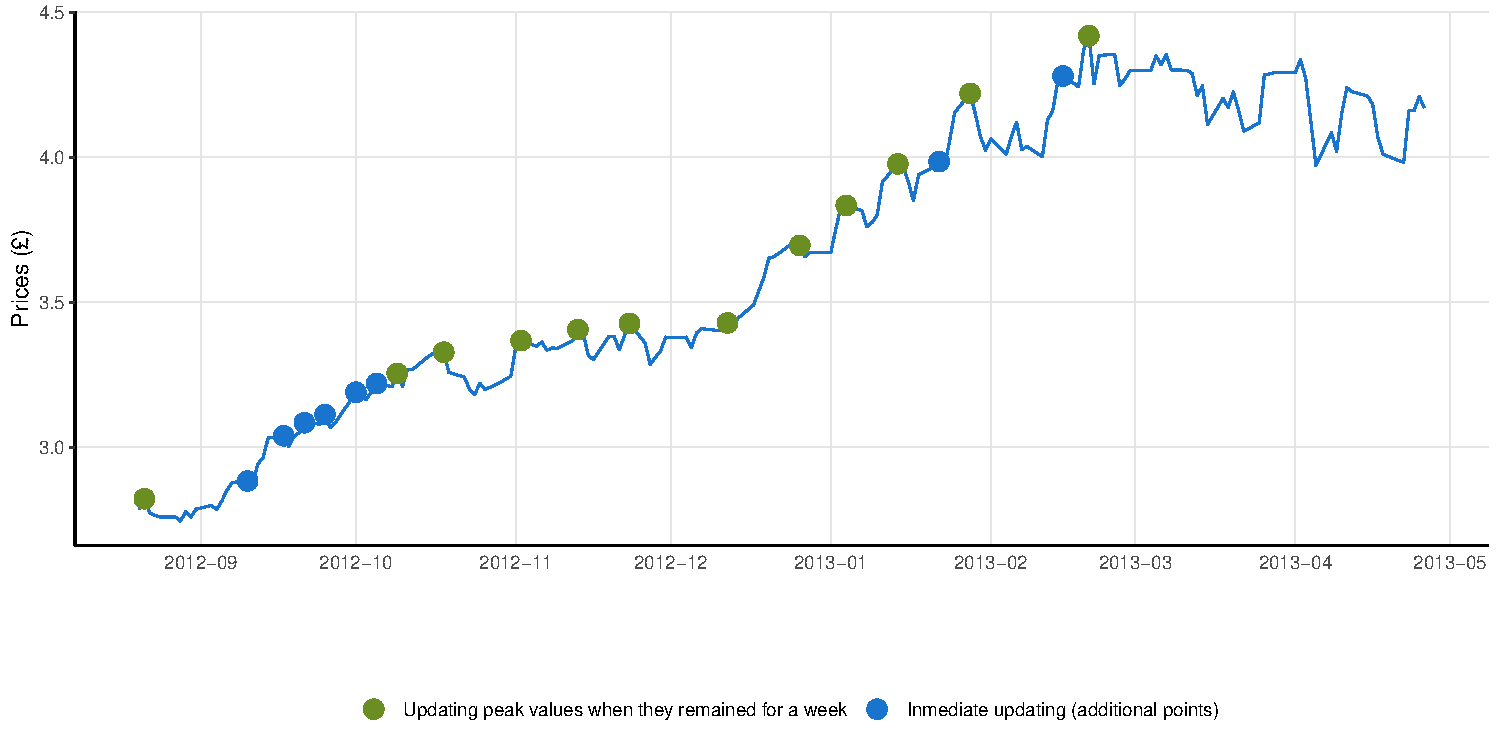
\includegraphics[width=0.7\textwidth]{figures/example_restriction_peaks_MAX.pdf}
	}
	\subfigure[Case 3: Peak has to be the highest price for at least a month]{	
		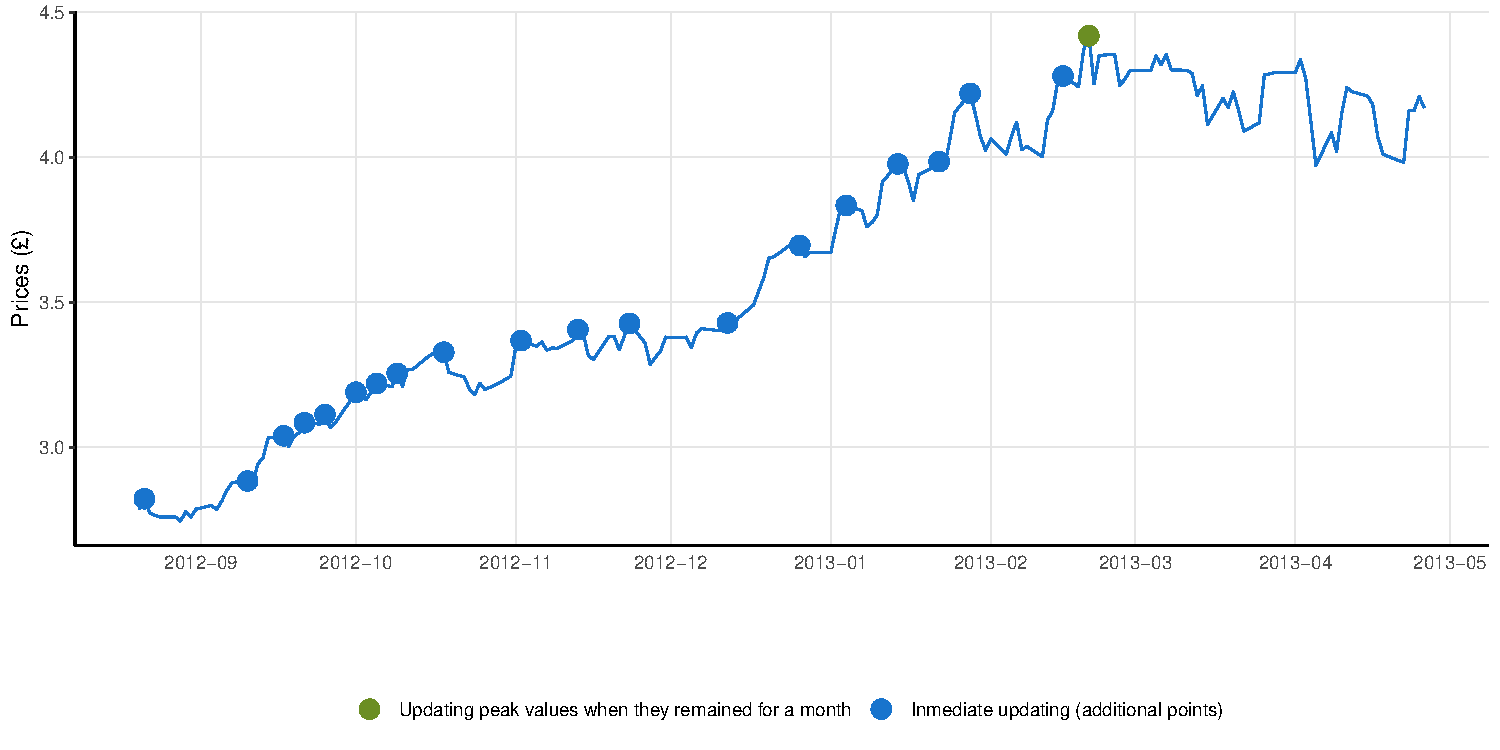
\includegraphics[width=0.7\textwidth]{figures/example_restriction_peaks_MAX20.pdf}
	}	
	\subfigure[Case 4: Peak has to be the highest price for at least a quarter ]{	
	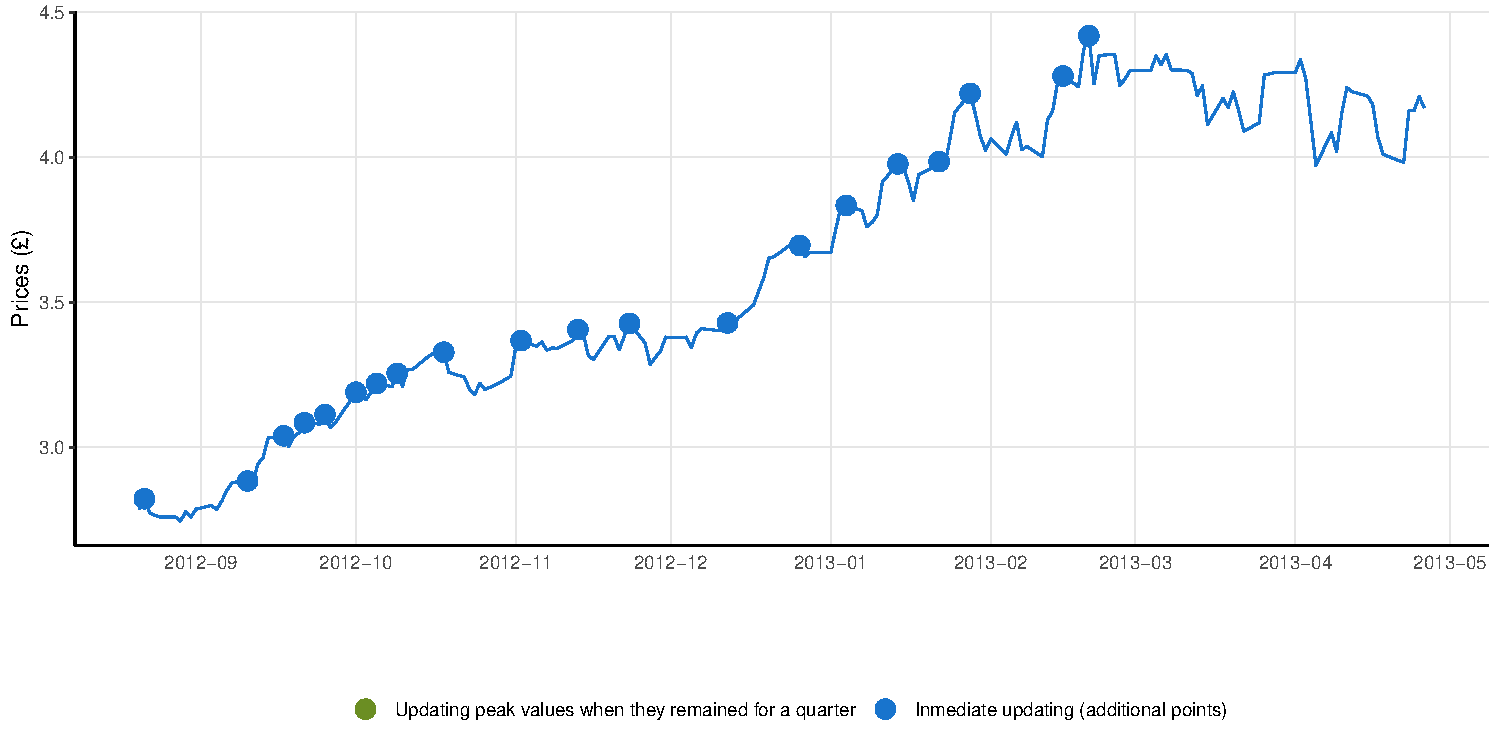
\includegraphics[width=0.7\textwidth]{figures/example_restriction_peaks_MAX60.pdf}
}
	\fignote{  }
\end{figure}
%%

\clearpage


\begin{figure}%
	\centering%
	\caption{DE Since Latest Peak Day}%
	\label{fig:DE_peak}%
		\subfigure[Case 1: Peak has to be the highest price]{	
		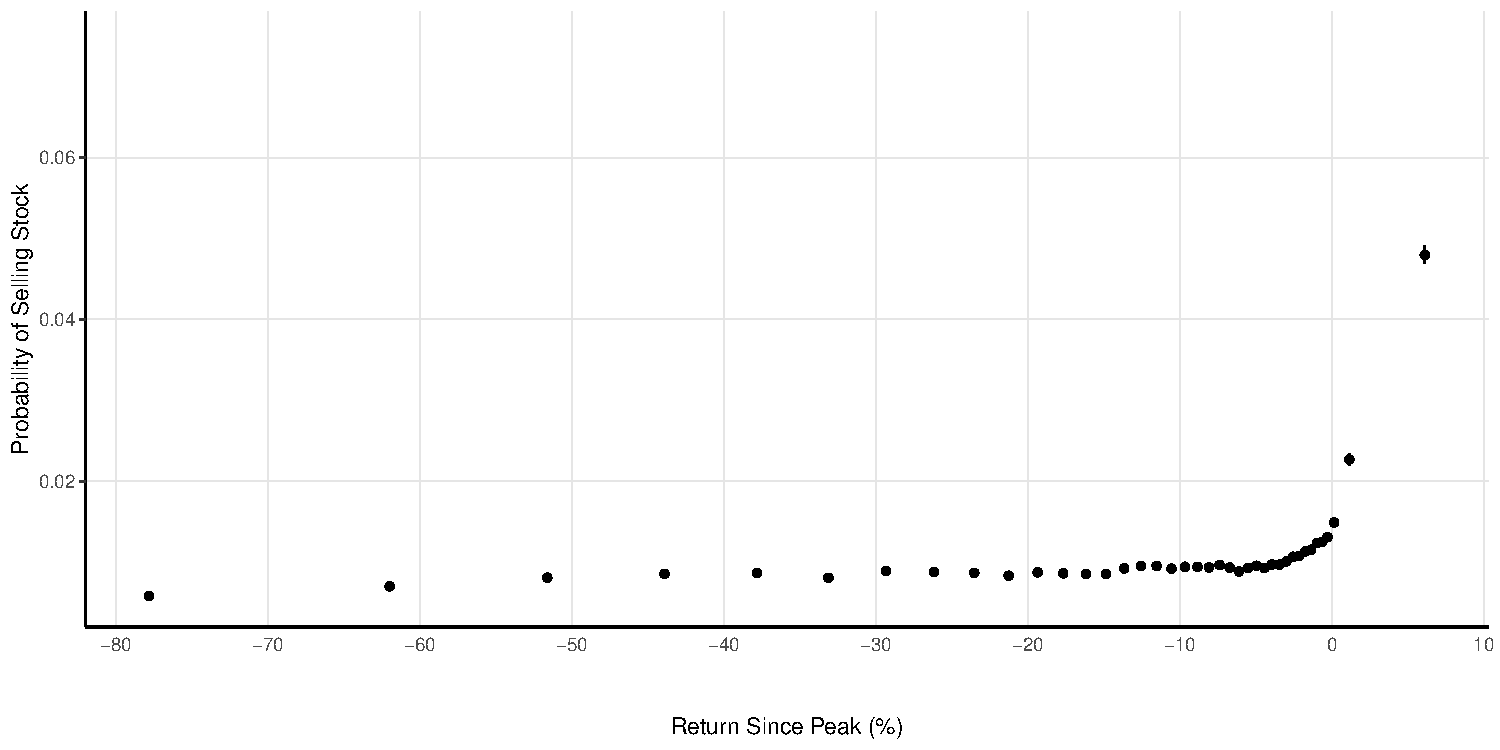
\includegraphics[width=0.6\textwidth]{figures/patter_DE_since_peak_window_year_login_sample2.pdf}
	}
	\subfigure[Case 2: Peak has to be the highest price for at least a week]{	
		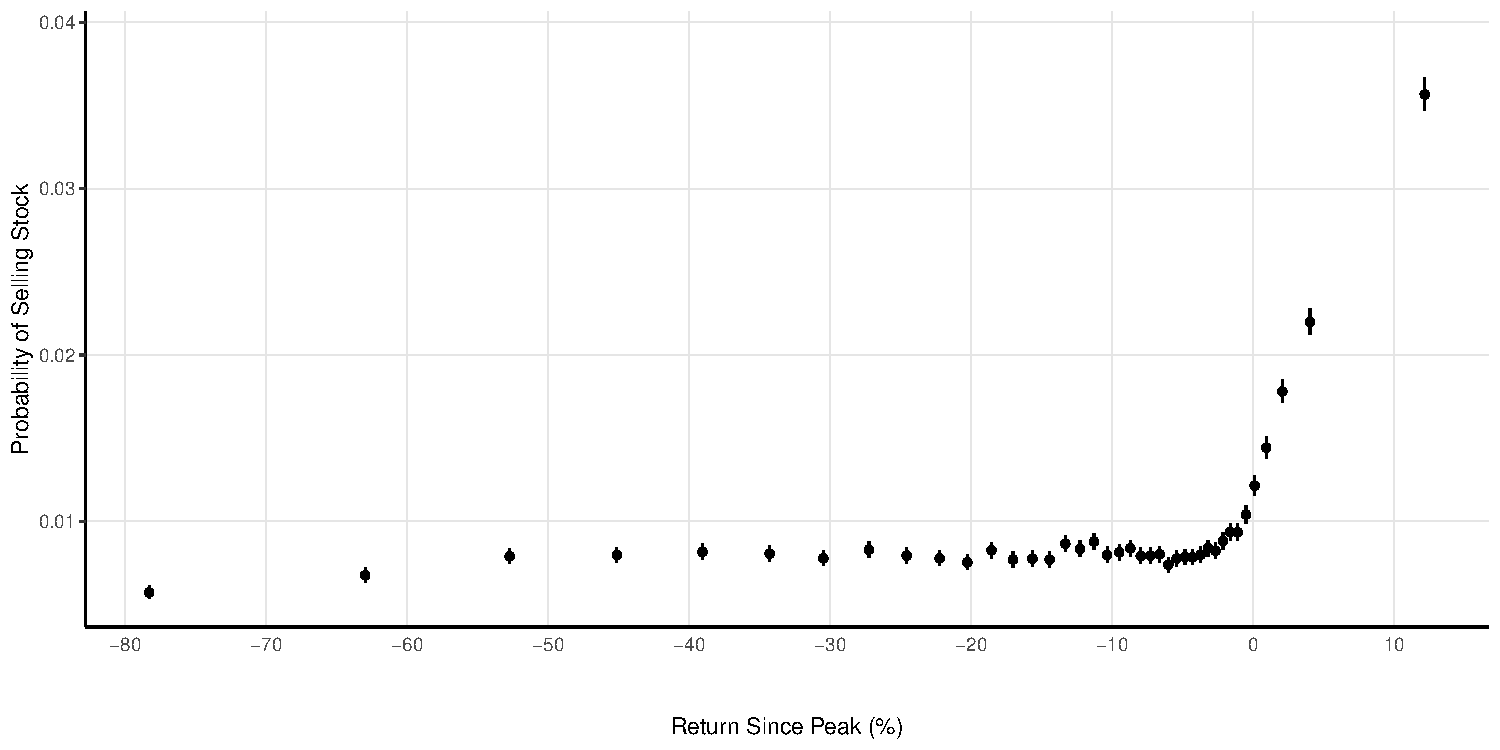
\includegraphics[width=0.6\textwidth]{figures/patter_DE_since_peak_window_year_login_sample_update_week2.pdf}
	}
	\subfigure[Case 3: Peak has to be the highest price for at least a month]{	
		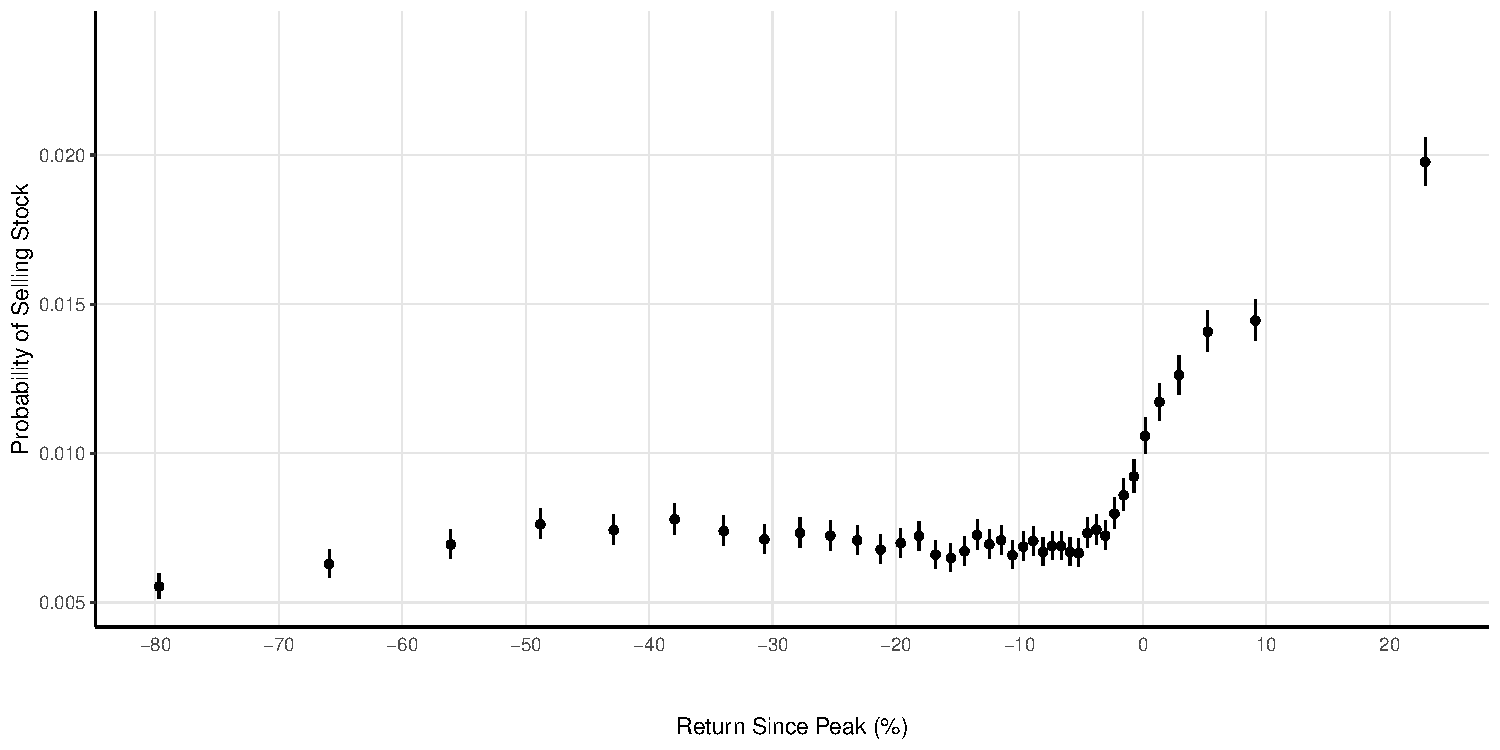
\includegraphics[width=0.6\textwidth]{figures/patter_DE_since_peak_window_year_login_sample_update_month2.pdf}
	}	
	\subfigure[Case 4: Peak has to be the highest price for at least a quarter ]{	
		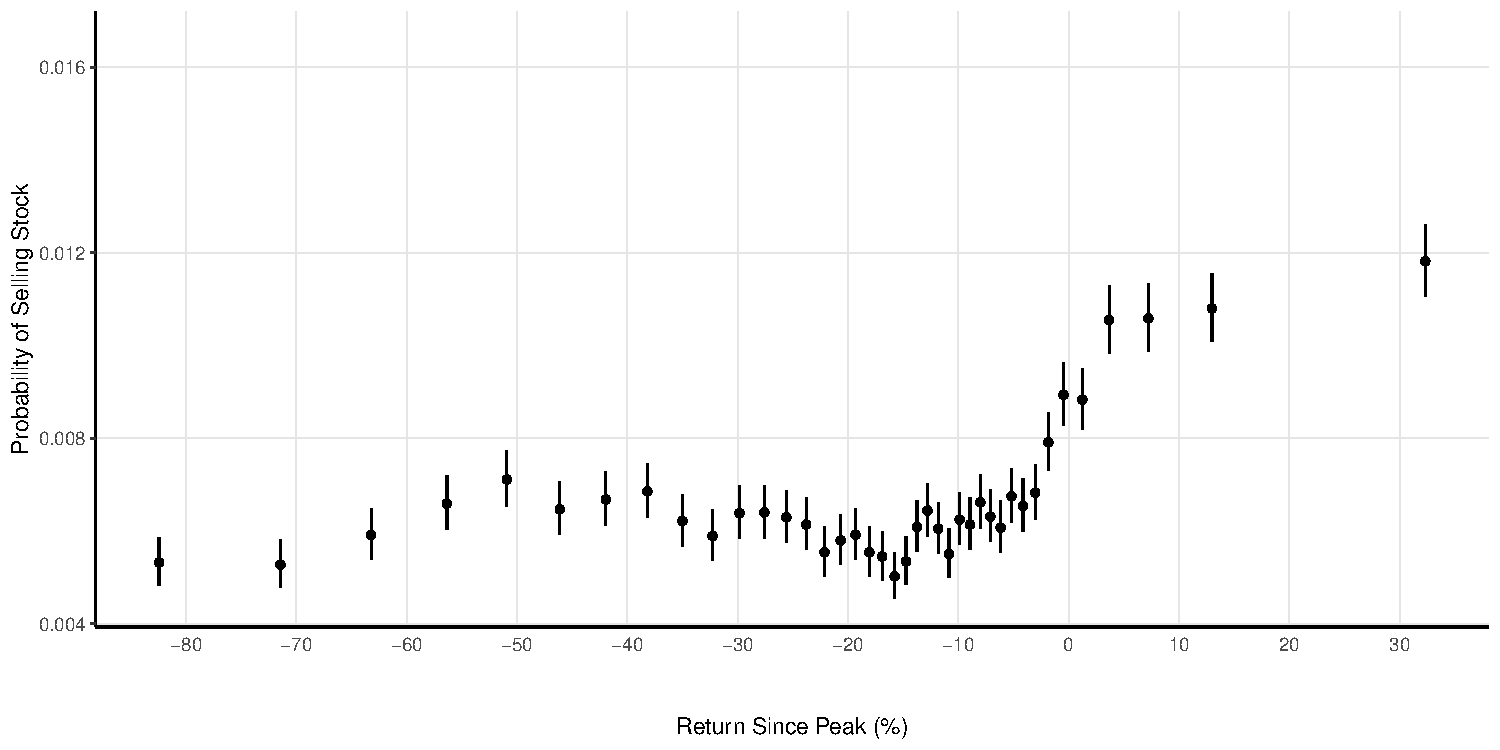
\includegraphics[width=0.6\textwidth]{figures/patter_DE_since_peak_window_year_login_sample_update_quarter2.pdf}
	}
	\fignote{  }
\end{figure}
%%

\clearpage


\begin{figure}%
	\centering%
	\caption{DE Since Latest Peak Day \& DE Since Purchase Day }%
	\label{fig:DE_peak_purc}%
	\subfigure[Case 1: Peak has to be the highest price]{	
		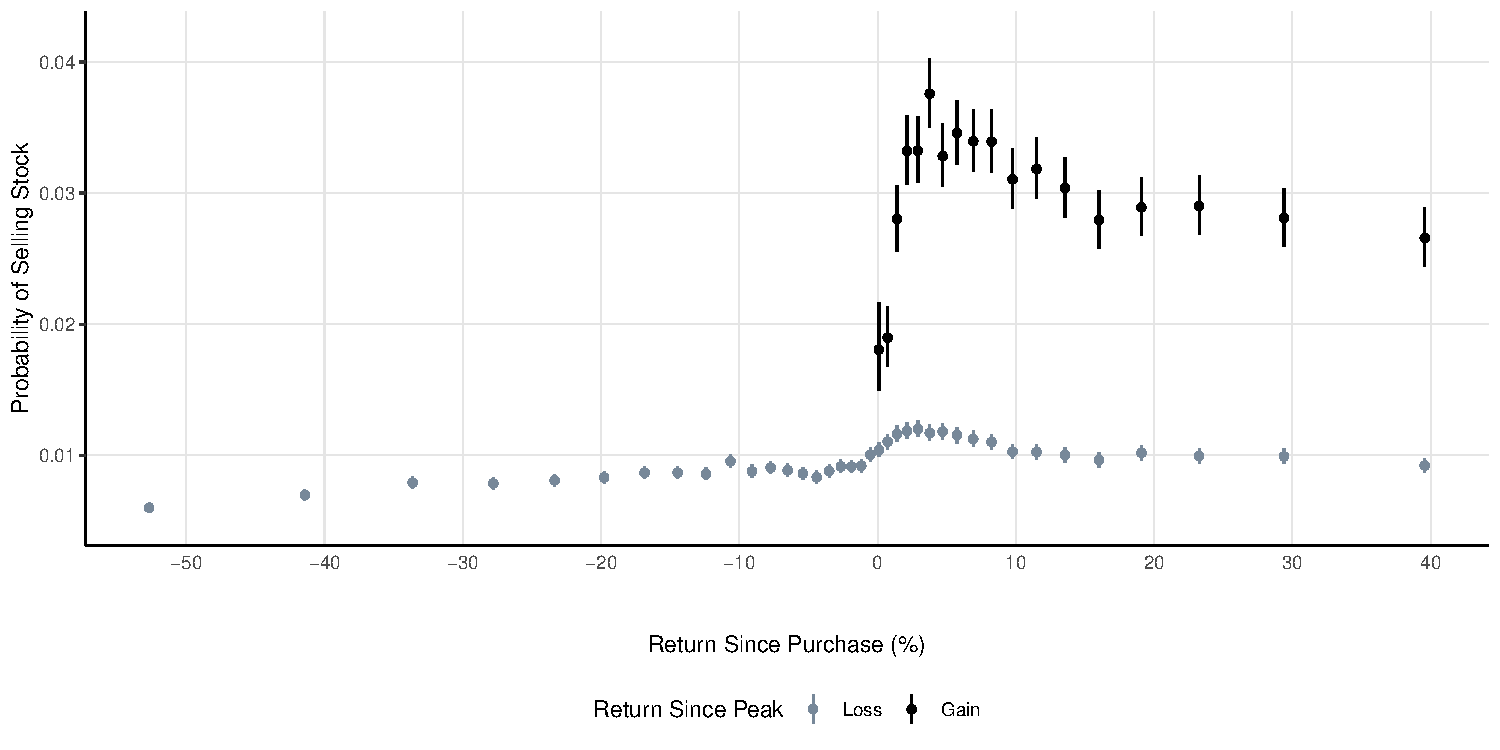
\includegraphics[width=0.6\textwidth]{figures/patter_DE_HOLDING_since_purch_peak_window_year_login_sample2_2.pdf}
	}
	\subfigure[Case 2: Peak has to be the highest price for at least a week]{	
		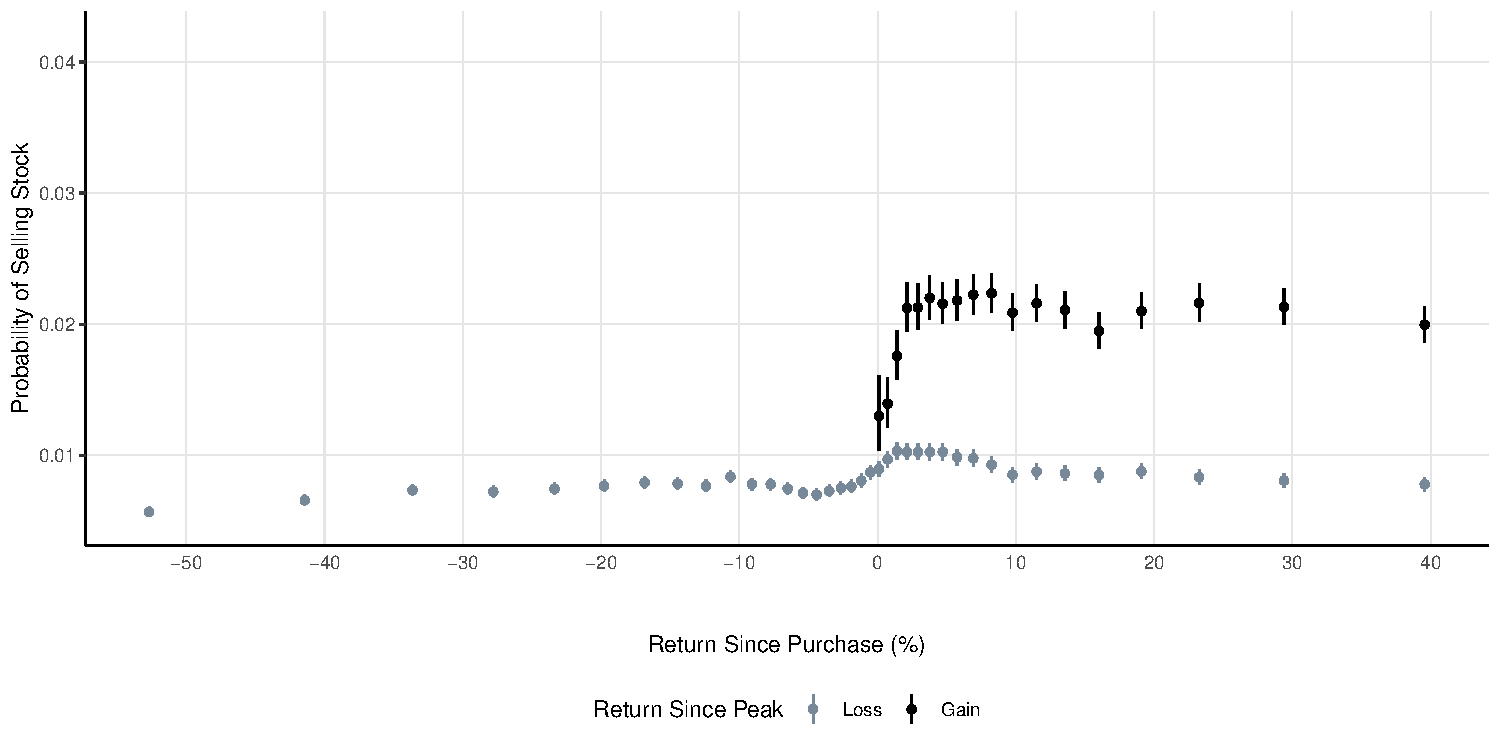
\includegraphics[width=0.6\textwidth]{figures/patter_DE_HOLDING_since_purch_peak_window_year_login_sample_update_week2_2.pdf}
	}
	\subfigure[Case 3: Peak has to be the highest price for at least a month]{	
		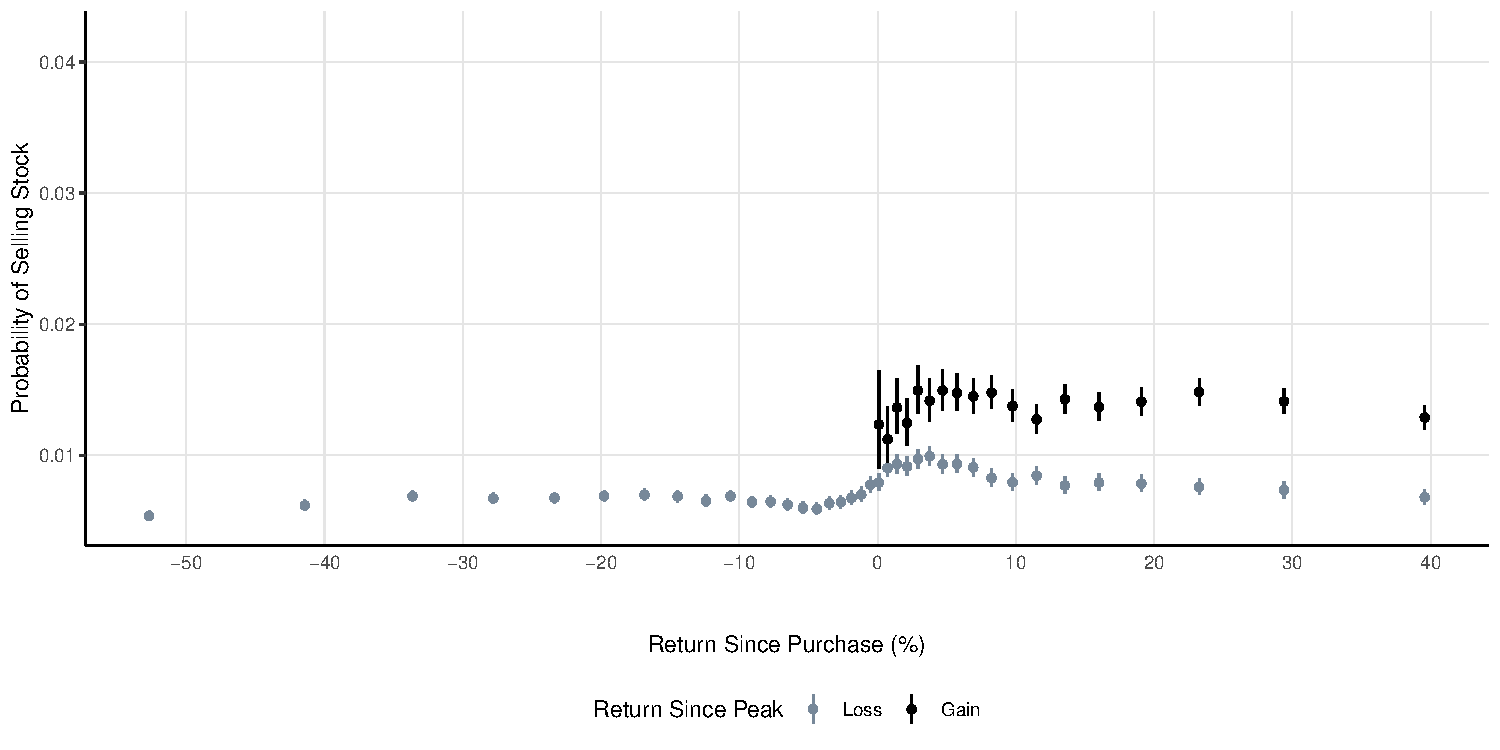
\includegraphics[width=0.6\textwidth]{figures/patter_DE_HOLDING_since_purch_peak_window_year_login_sample_update_month2_2.pdf}
	}	
	\subfigure[Case 4: Peak has to be the highest price for at least a quarter ]{	
		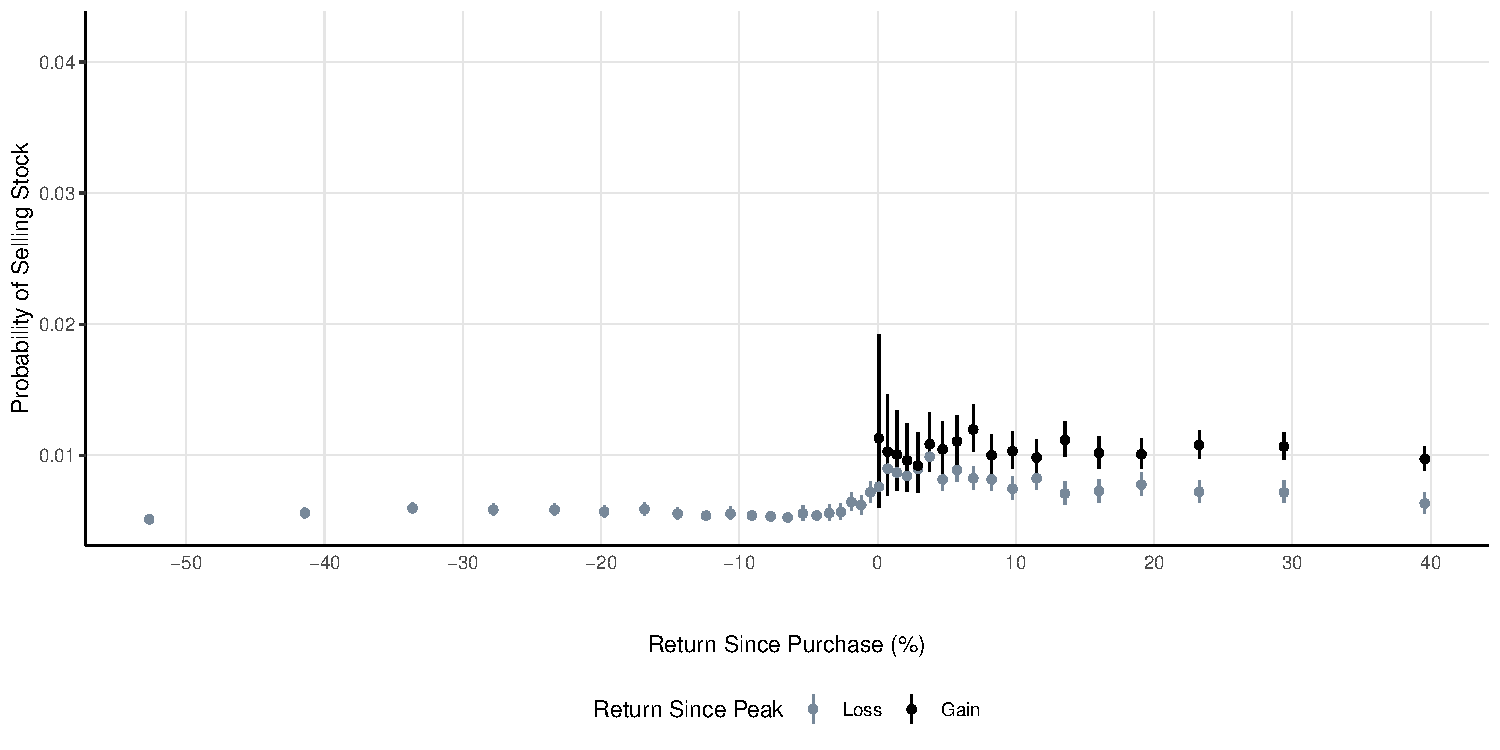
\includegraphics[width=0.6\textwidth]{figures/patter_DE_HOLDING_since_purch_peak_window_year_login_sample_update_quarter2_2.pdf}
	}
	\fignote{  }
\end{figure}
%%

\clearpage



\begin{figure}%
	\centering%
	\caption{Distribution of Returns Since Peak Day }%
	\label{fig:hist_return_peak}%
	\subfigure[Case 1: Peak has to be the highest price]{	
		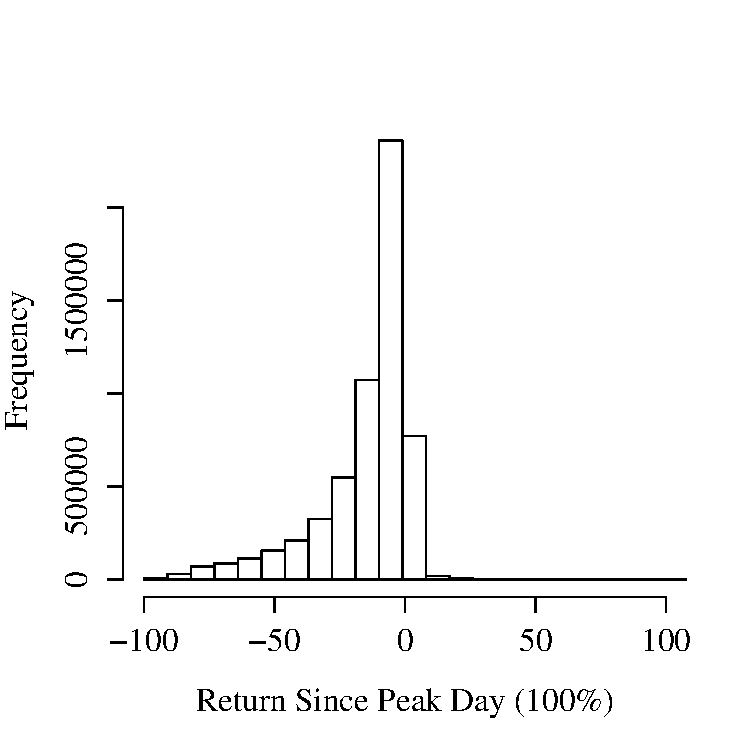
\includegraphics[width=0.6\textwidth]{figures/return_since_peak_MAX_inmediate_updated.pdf}
	}
		\subfigure[Case 4: Peak has to be the highest price for at least a quarter ]{	
		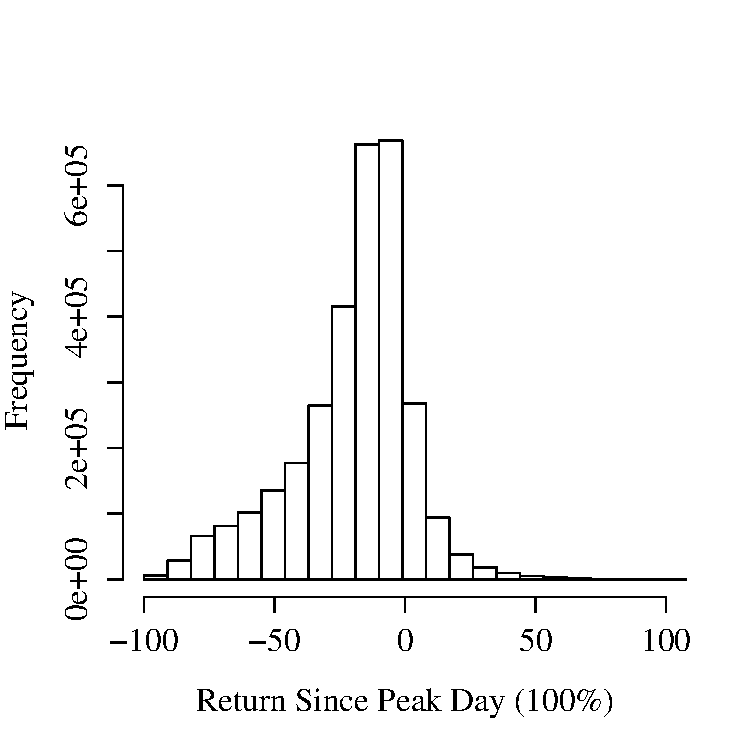
\includegraphics[width=0.6\textwidth]{figures/return_since_peak_MAX_inmediate_quarter_updated.pdf}
	}
	\fignote{  }
\end{figure}

\clearpage
\clearpage

\section{Selling patterns when the peak price is the highest price in the past year}

In the earlier section, the investor hold the stocks during the peak days and the gain since peak price was much more stronger than the gain since purchase. In this section, peaks days happen in the past year and could happen before the purchase day.

\subsection{Definition of Peak Prices}
For simplicity, I have analysed only two cases. 

\begin{itemize}
	\item Case 1: The peak price is the highest price in the past year (independently on whether the investo hold the stock or not). The only requirement is that the day before (and the day after) the peak day the price have to be smaller than during the peak day. In this case, if an stock has crossed a peak price yesterday, the price yesterday could become a new peak price tomorrow if today the price has gone down.
	
	
	\item Case 2: The potential peak value has to be the highest price for at least a week to be considerer a peak price.

	
\end{itemize}

I have not included cases 3 and 4 because the same conclusions from the last section apply also here (so the effect of a gain since the peak price day is smaller when we have fewer peak values) 

\ref{fig:example_peak_window} shows another example of peak points comparing Case 1 (blue and green points are peak prices) with Case 2 (only green points are peak prices).

\begin{figure}[h]%
	\centering%
	\caption{Example Peak Prices  \\
		Comparison of Peak Prices for Case 2 against Case 1}%
	\label{fig:example_peak_window}%
		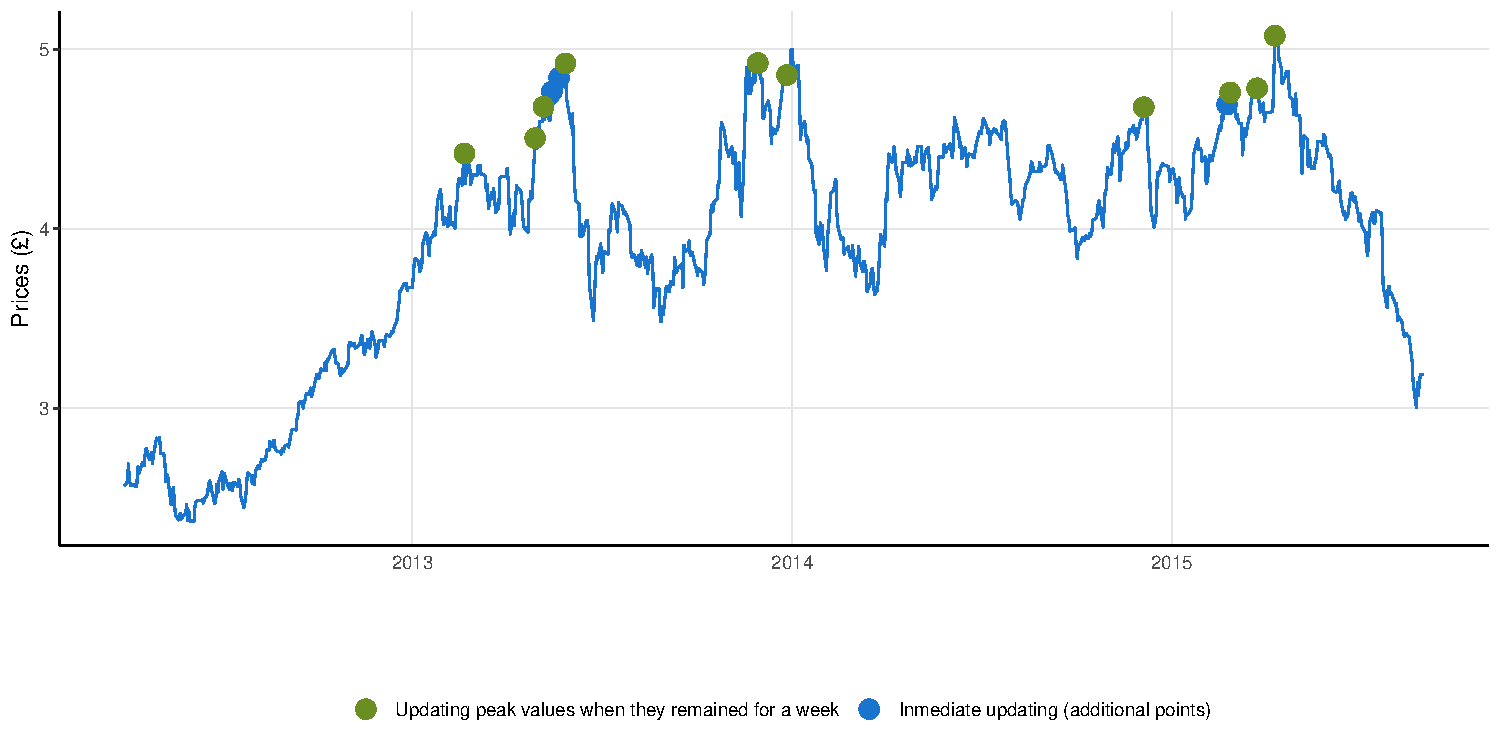
\includegraphics[width=0.7\textwidth]{figures/example_restriction_peaks.pdf}
	\fignote{  }
\end{figure}

\subsection{Disposition Effect Since Latest Peak Price Day}

\ref{fig:DE_since_peak_window} shows the DE since peak price. We see a jump around zero returns. In \ref{fig:de_peak_holding_window} we see how these patterns change when the investor hold or not the stock.

In \ref{fig:example_peak_gain_loss}, I have included some random examples of login days (Day t) for when an stock is in gain or loss since the past peak price. 

\subsubsection{Losses Since Peak Price Day} 
In \ref{fig:de_peak_holding_window}, we observe that \textcolor{blue}{\textbf{when the investor has experienced the peak price and is now in loss since that peak, he is reluctant to sell}} (black points, left side of zero) (for some examples, see \ref{fig:example_peak_gain_loss}, Plots A and B, days following the Peak Day. But note that Plot A is a rare pattern.) 

However, when the peak price occurred before purchasing the stock and the stock is today in loss since that peak, the investor might make some sells (grey points, left side of zero) (See \ref{fig:example_peak_gain_loss}, Plot D, days after the purchase day and before Day t). Perhaps the peak price is not that important for the investor and he does not feel a real loss. 

All these days with loss since the peak price day could be a gain or a loss since purchase. 

\subsubsection{Gains Since Peak Day} 
Now, \textcolor{blue}{\textbf{when the investor has experienced the peak price and is now in gain since that peak (black points, right side of zero) he is selling. These days are always a gain since purchase (See \ref{fig:example_peak_gain_loss}, Plot B, Day t for instance). \\
But when the peak price occurred before purchasing the stock and the stock is today in gain since that peak, the investor is making even more sells}} (grey points, right side of zero in \ref{fig:de_peak_holding_window}). These days are always a gain since purchase for Case 1. For Case 2, there are few days in which the stock could be in loss since purchase and in gain since the peak price day if a higher price than the peak price has happened before the purchase day but was not considered a peak price--- because it was not the highest price for at least a week. For example, see \ref{fig:example_peak_gain_loss}, Plot C, the prices before the purchase day. But these are very rare events and most days with gains since the peak price day are also days with gains since purchase. 


\textcolor{blue}{\textbf{I am puzzled with this result. Why there is a jump when the stock has crossed a peak that occurred before the purchase day? Part of this jump is explained because stocks are a gain since purchase. But why people would sell more under Plot D (on Day t) than under Plot B (on Day t)? Perhaps beating a past peak that happened long time ago feels more incredible that people want to realize the gain as soon as possible?}}



\begin{figure}%
	\centering%
	\caption{DE Since Latest Peak Day}%
	\label{fig:DE_since_peak_window}%
	\subfigure[Case 1: Peak has to be the highest price in the past year]{	
		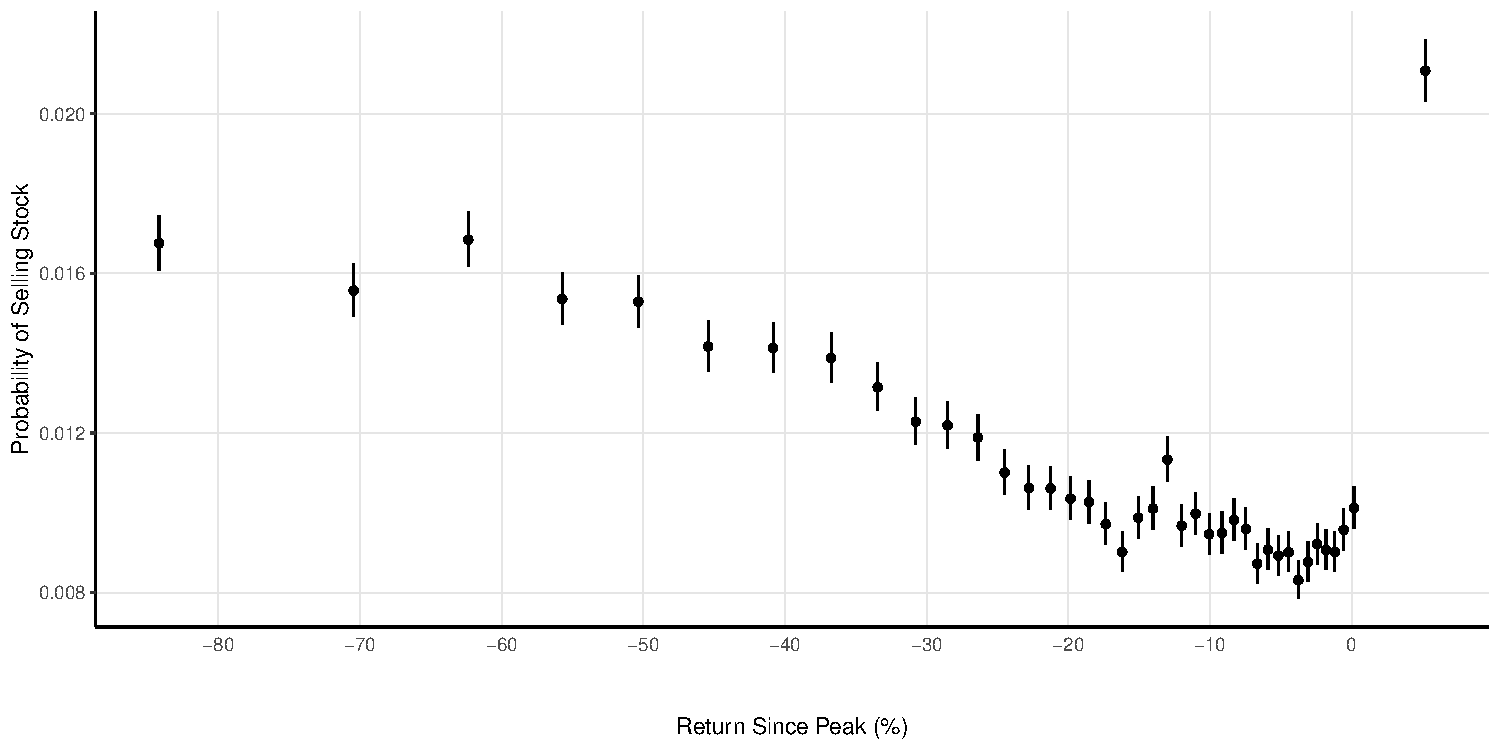
\includegraphics[width=0.7\textwidth]{figures/patter_DE_since_peak_window_year_login_sample.pdf}
	}	
	\subfigure[Case 2: Peak has to be the highest price in the past year for at least a week ]{	
		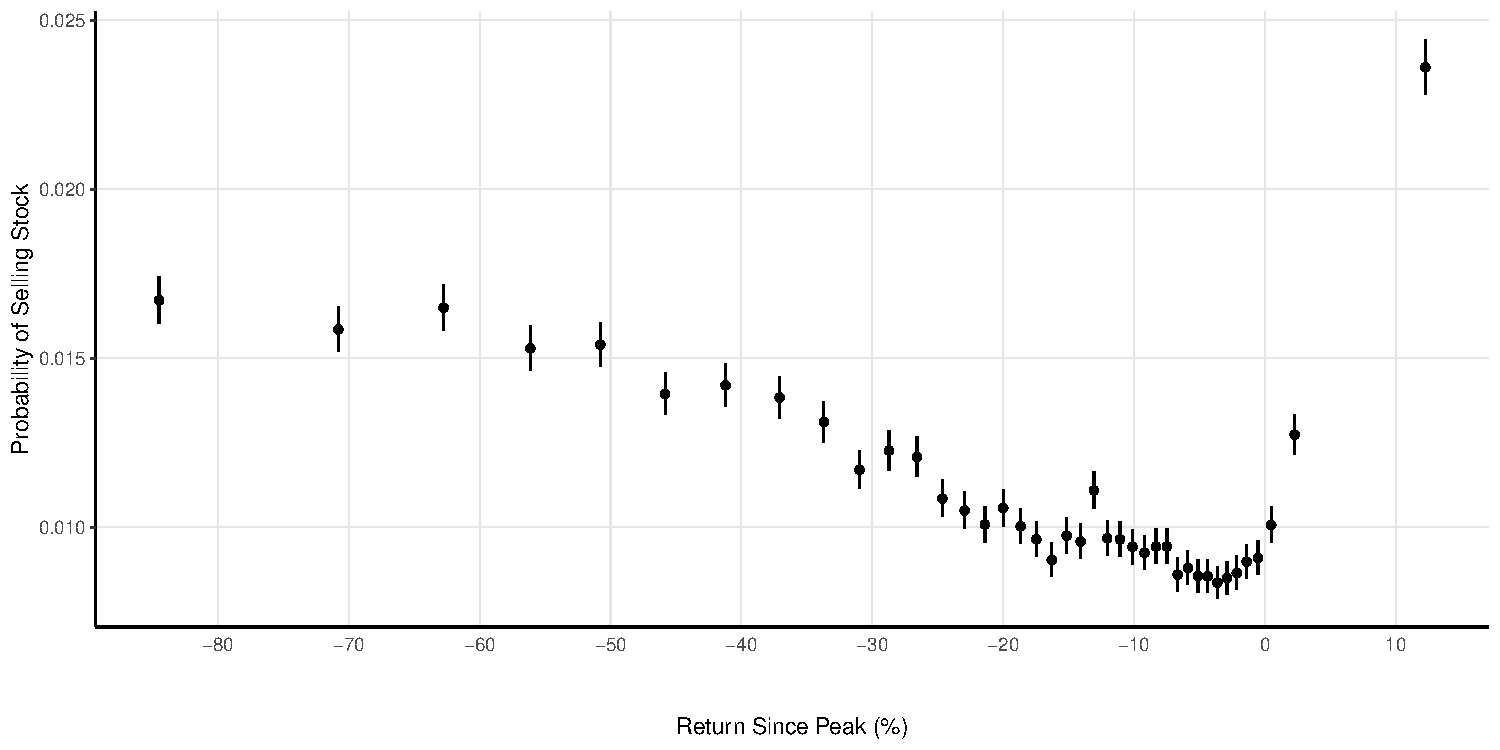
\includegraphics[width=0.7\textwidth]{figures/patter_DE_since_peak_window_year_login_sample_update_week.pdf}
	}
	\fignote{  }
\end{figure}

\begin{figure}%
	\centering%
	\caption{DE Since Latest Peak Day}%
	\label{fig:de_peak_holding_window}%
	\subfigure[Case 1: Peak has to be the highest price in the past year]{	
		\includegraphics[width=0.7\textwidth]{figures/patter_DE_HOLDING_since_peak_window_year_login_sample.pdf}
	}	
	\subfigure[Case 2: Peak has to be the highest price in the past year for at least a week ]{	
		\includegraphics[width=0.7\textwidth]{figures/patter_DE_HOLDING_since_peak_window_year_login_sample_update_week.pdf}
	}
	\fignote{  }
\end{figure}


\begin{figure}%
	\centering%
	\caption{Examples of Days with Gains Since Purchase Day or Gains Since Peak Day}%
	\label{fig:example_peak_gain_loss}%
	\subfigure[Holding Stock on Peak Day - Loss Since Purchase - Gain Since Peak]{	
		\includegraphics[width=0.7\textwidth]{figures/hold_gainpeak_losspurch.pdf}
	}	
	\subfigure[Holding Stock on Peak Day - Gain Since Purchase - Gain Since Peak ]{	
		\includegraphics[width=0.7\textwidth]{figures/hold_gainpeak_gainpurch.pdf}
	}
	\subfigure[No Holding Stock on Peak Day - Loss Since Purchase - Gain Since Peak (Only for Case 2)]{	
		\includegraphics[width=0.7\textwidth]{figures/nohold_gainpeak_losspurch_update_week.pdf}
	}	
	\subfigure[No Holding Stock on Peak Day - Gain Since Purchase - Gain Since Peak ]{	
		\includegraphics[width=0.7\textwidth]{figures/nohold_gainpeak_gainpurch.pdf}
	}
	\fignote{Across panels, Day t reflects examples of login days with a gain or loss since the past peak day. Panels A, B and D correspond to Case 1, and only Panel C, to Case 2.    }
\end{figure}

\clearpage
\subsection{DE Since Purchase Day vs Holding the Stock During the Peak Price Day}

\textcolor{blue}{In \ref{fig:DE_purch_holding}, we see that when a peak day happened after the purchase of the stock, the DE since purchase is almost vanished. See the horinzontal black lines. So the price on the peak day might have replace the purchase price in peoples' mind.}


 

 
\begin{figure}[h]%
	\centering%
	\caption{DE Effect Since Purchase Day}%
	\label{fig:DE_purch_holding}%
	\subfigure[Case 1: Peak has to be the highest price in the past year]{	
		\includegraphics[width=0.7\textwidth]{figures/patter_DE_HOLDING_since_purch_window_year_login_sample.pdf}
	}	
	\subfigure[Case 2: Peak has to be the highest price in the past year for at least a week ]{	
		\includegraphics[width=0.7\textwidth]{figures/patter_DE_HOLDING_since_purch_window_year_login_sample_update_week.pdf}
	}
	\fignote{  }
\end{figure}

\textcolor{blue}{Above we are not considering whether the stock is in gain since the peak price. But in \ref{fig:DE_pur_peak_hold} we see that this reduction of the DE since purchase (only when the peak price day occurred after the purchase of the stock) happens when the stock is in loss since the peak price day. See the flat grey lines on the right panels. The left panels show, however, than when the peak price happened before the purchase day, the purchase price still has an effect on selling decisions.}

The right panels (for when the investor hold the stock during the peak price day) very much agree with the results of the earlier section that defines peak prices as the highest price since purchase. So a loss  since the peak price day vanishes the effect of the purchase price.

There are very few observations with gain since peak day and loss since purchase day. So the confidence intervals for these events are huge. Example of these rare events are in \ref{fig:example_peak_gain_loss}. For Case 1, see Plot A and Day t; and for Case 2, see Plot C and Day t. Perhaps we can make exclude these points for the main analysis and show the full figures in an Appendix? \\



\begin{figure}[h]%
	\centering%
	\caption{DE Since Purchase  Day}%
	\label{fig:DE_pur_peak_hold}%
	\subfigure[Case 1: Peak has to be the highest price in the past year]{	
		\includegraphics[width=0.7\textwidth]{figures/patter_DE_HOLDING_since_purch_peak_window_year_login_sample2.pdf}
	}	
	\subfigure[Case 2: Peak has to be the highest price in the past year for at least a week]{	
		\includegraphics[width=0.7\textwidth]{figures/patter_DE_HOLDING_since_purch_peak_window_year_login_sample_update_week2.pdf}
	}
	\fignote{  }
\end{figure}
%ggsave("patter_DE_HOLDING_since_purch_peak_window_year_login_sample2.pdf", width = 10, height = 5)
%ggsave("patter_DE_HOLDING_since_purch_peak_window_year_login_sample_update_week2.pdf", width = 10, height = 5)


\clearpage
\textcolor{blue}{\textbf{Points to discuss for the study of the maximum peak price experienced by the investor : 
		\begin{itemize}
			\item Which definition of peak price to use? We do not want to add subjective restrictions that a reviewer my question, but Case 1 has many peak values that happened on day t-2. I would prefer to use the definition given by Case 2 (peak price has to be the highest price for at least one week).
			\item We planned to follow the same regression used for the DE paper. So regressing sells on a dummy for gain since purchase, a dummy for gain since peak price day and the interaction between the dummies. But because all days with \textit{ gain since peak price day = 1} are also days with \textit{ gain since purchase day = 1}, the interaction is going to give me the EXACT SAME vector of the \textit{gain since peak price day} dummy. So it makes no sense to control for the independent effects and the interaction---the dummy for \textit{gain since peak price day} is already telling us the effect of having both gains occurring on the same day.
			Then, our focus has to be in the coefficient of the \textit{gain since peak price day} dummy, which we expect to be positive. \\
\end{itemize}}}		




\textcolor{blue}{\textbf{Points to discuss for the study of the maximum peak price in the past year: 
		\begin{itemize}
			\item Again, which definition of peak price to use? 
			\item Since the focus here is on the effect of holding the stock, I think we should do first a regression interacting the \textit{gain since purchase day} with a dummy for holding the stock when the peak price happened. Then, the same regressions described in the previous points but for two separate samples (holding or not the stock). I have done some preliminary analysis in the next pages, using the definition of peak prices in Case 2 (Case 1 will give bigger effects). 	
			\item Because in this setting it is possible to have a \textit{gain since peak price day=1} and a \textit{gain since purchase =0}, see Plot A in \ref{fig:example_peak_gain_loss}, technically we can add the interaction of  both dummies for gains because there is no perfect multicollinearity. But it makes no sense to do so. The interaction is highly collinear with the \textit{gain since peak price day} dummy and the  coefficients of these two variables are going to be unstable. I have added these results just to show you why we should not include this interaction. 
			\item Because cases with  \textit{gain since peak price day=1} and a \textit{gain since purchase =0} are very rare, I think we should exclude them. 
\end{itemize}}}



%regressions
\clearpage
\textcolor{blue}{We start by looking at the maximum price experienced by the investor. See in column 3 that a gain since the peak price day has a positive coefficient. }

\begin{econtable}[h]\footnotesize
	\caption{DE Since Latest Peak Price Day \\ (Case 2: Peak has to be the highest price experienced for at least a week) }
	\label{tab:}
	\estauto{l c c c c   }{
		& \multicolumn{3}{c}{$Probability\:  of\:  Sale_{ijt}=1$} \\ 
		%	\cmidrule(rr){2-7}
		& \multicolumn{1}{c}{(1)} & \multicolumn{1}{c}{(2)} & \multicolumn{1}{c}{(3)} & \\ 
		\midrule
		 Gain Since Purchase=1 & 0.0060{***} &  & 0.0018{***} \\ 
  & (0.0004) &  & (0.0002) \\ 
  & & & \\ 
 Gain Since Latest Peak Price=1 &  & 0.0129{***} & 0.0118{***} \\ 
  &  & (0.0006) & (0.0005) \\ 
  & & & \\ 
 Constant & 0.0086{***} & 0.0081{***} & 0.0074{***} \\ 
  & (0.0002) & (0.0002) & (0.0002) \\ 
  & & & \\ 
Observations & \multicolumn{1}{c}{5,840,342} & \multicolumn{1}{c}{5,478,072} & \multicolumn{1}{c}{5,478,072} \\ 
R$^{2}$ & \multicolumn{1}{c}{0.0008} & \multicolumn{1}{c}{0.0018} & \multicolumn{1}{c}{0.0018} \\ 
 
	}
	\fignote{The unit of observation is an investor $\times$ stock $\times$ day. The samples is restricted to login days. SE clustered by account and day.}
\end{econtable}



\clearpage
\textcolor{blue}{Now we moved to the maximum price in the past year. Regressions in the next tables are omitting the observations with \textit{gain since peak price day=1} and a \textit{gain since purchase =0}. The effect of the gain since peak price day dummy in column 2 is just capturing the effect of a gain since purchase. See that the effect of the peak price in column 3 is only relevant when holding the stock during the peak price day.   }

\begin{econtable}[h]\footnotesize
	\caption{DE Since Latest Peak Price Day \\\textbf{ No Holding Stock on Peak Price Day} \\ (Case 2: Peak has to be the highest price in the past year for at least a week) }
	\label{tab:}
	\estauto{l c c c c   }{
		& \multicolumn{3}{c}{$Probability\:  of\:  Sale_{ijt}=1$} \\ 
		%	\cmidrule(rr){2-7}
		& \multicolumn{1}{c}{(1)} & \multicolumn{1}{c}{(2)} & \multicolumn{1}{c}{(3)} & \\ 
		\midrule
		 Gain Since Purchase=1 & 0.0160{***} &  & 0.0159{***} \\ 
  & (0.0007) &  & (0.0008) \\ 
  & & & \\ 
 Gain Since Latest Peak Price=1 &  & 0.0118{***} & 0.0012 \\ 
  &  & (0.0011) & (0.0011) \\ 
  & & & \\ 
 Constant & 0.0100{***} & 0.0154{***} & 0.0100{***} \\ 
  & (0.0003) & (0.0004) & (0.0003) \\ 
  & & & \\ 
Observations & \multicolumn{1}{c}{2,589,709} & \multicolumn{1}{c}{2,589,709} & \multicolumn{1}{c}{2,589,709} \\ 
R$^{2}$ & \multicolumn{1}{c}{0.0038} & \multicolumn{1}{c}{0.0003} & \multicolumn{1}{c}{0.0038} \\ 
 
	}
	\fignote{The unit of observation is an investor $\times$ stock $\times$ day. The samples is restricted to login days. SE clustered by account and day.}
\end{econtable}




\begin{econtable}[h]\footnotesize
	\caption{DE Since Latest Peak Price Day \\\textbf{ Holding Stock on Peak Price Day} \\ (Case 2: Peak has to be the highest price in the past year for at least a week) }
	\label{tab:}
	\estauto{l c c c c   }{
		& \multicolumn{3}{c}{$Probability\:  of\:  Sale_{ijt}=1$} \\ 
		%	\cmidrule(rr){2-7}
		& \multicolumn{1}{c}{(1)} & \multicolumn{1}{c}{(2)} & \multicolumn{1}{c}{(3)} & \\ 
		\midrule
		 Gain Since Purchase=1 & 0.0017{***} &  & 0.0008{***} \\ 
  & (0.0002) &  & (0.0002) \\ 
  & & & \\ 
 Gain Since Latest Peak Price=1 &  & 0.0053{***} & 0.0048{***} \\ 
  &  & (0.0004) & (0.0004) \\ 
  & & & \\ 
 Constant & 0.0063{***} & 0.0067{***} & 0.0063{***} \\ 
  & (0.0002) & (0.0002) & (0.0002) \\ 
  & & & \\ 
Observations & \multicolumn{1}{c}{2,856,939} & \multicolumn{1}{c}{2,856,939} & \multicolumn{1}{c}{2,856,939} \\ 
R$^{2}$ & \multicolumn{1}{c}{0.0001} & \multicolumn{1}{c}{0.0004} & \multicolumn{1}{c}{0.0004} \\ 
 
	}
	\fignote{The unit of observation is an investor $\times$ stock $\times$ day. The samples is restricted to login days. SE clustered by account and day.}
\end{econtable}


\clearpage
\textcolor{blue}{Here I repeated the previous regressions but I do not omit any observation. So it was possible to include the interaction. The coefficients in column 4 are unreliable because of the high degree of multicollinearity between the interaction and the dummy for gain since peak price day. Also, see in column 3 that a gain since the peak price day matters even when no holding the stock during that day. But this result is just an effect of the rare events that I omitted in the previous tables. This positive coefficient is affected by the rare events in  \ref{fig:DE_pur_peak_hold}, Plot B, left side,  days with \textit{gain since peak price day=1} and a \textit{gain since purchase =0}   }



\begin{econtable}[h]\footnotesize
	\caption{DE Since Latest Peak Price Day \\\textbf{ No Holding Stock on Peak Price Day} \\ (Case 2: Peak has to be the highest price in the past year for at least a week) }
	\label{tab:}
	\estauto{l c c c c c  }{
		& \multicolumn{4}{c}{$Probability\:  of\:  Sale_{ijt}=1$} \\ 
		%	\cmidrule(rr){2-7}
		& \multicolumn{1}{c}{(1)} & \multicolumn{1}{c}{(2)} & \multicolumn{1}{c}{(3)} &  \multicolumn{1}{c}{(4)} & \\ 
		\midrule
		 Gain Since Purchase=1 & 0.0158{***} &  & 0.0154{***} & 0.0159{***} \\ 
  & (0.0007) &  & (0.0008) & (0.0008) \\ 
  & & & & \\ 
 Gain Since Latest Peak Price=1 &  & 0.0131{***} & 0.0048{***} & 0.0274{***} \\ 
  &  & (0.0011) & (0.0012) & (0.0032) \\ 
  & & & & \\ 
 Gain Since Purchase=1 $\times$ Gain Since Lastest Peak Price=1 &  &  &  & -0.0262{***} \\ 
  &  &  &  & (0.0031) \\ 
  & & & & \\ 
 Constant & 0.0102{***} & 0.0154{***} & 0.0102{***} & 0.0100{***} \\ 
  & (0.0003) & (0.0004) & (0.0003) & (0.0003) \\ 
  & & & & \\ 
Observations & \multicolumn{1}{c}{2,601,643} & \multicolumn{1}{c}{2,601,643} & \multicolumn{1}{c}{2,601,643} & \multicolumn{1}{c}{2,601,643} \\ 
R$^{2}$ & \multicolumn{1}{c}{0.0037} & \multicolumn{1}{c}{0.0004} & \multicolumn{1}{c}{0.0037} & \multicolumn{1}{c}{0.0039} \\ 
 
	}
	\fignote{The unit of observation is an investor $\times$ stock $\times$ day. The samples is restricted to login days. SE clustered by account and day.}
\end{econtable}




\begin{econtable}[h]\footnotesize
	\caption{DE Since Latest Peak Price Day \\\textbf{ Holding Stock on Peak Price Day} \\ (Case 2: Peak has to be the highest price in the past year for at least a week) }
	\label{tab:}
	\estauto{l c c c c c  }{
		& \multicolumn{4}{c}{$Probability\:  of\:  Sale_{ijt}=1$} \\ 
		%	\cmidrule(rr){2-7}
		& \multicolumn{1}{c}{(1)} & \multicolumn{1}{c}{(2)} & \multicolumn{1}{c}{(3)} & \multicolumn{1}{c}{(4)} & \\ 
		\midrule
		 Gain Since Purchase=1 & 0.0017{***} &  & 0.0008{***} & 0.0008{***} \\ 
  & (0.0002) &  & (0.0002) & (0.0002) \\ 
  & & & & \\ 
 Gain Since Latest Peak Price=1 &  & 0.0053{***} & 0.0049{***} & 0.0109{***} \\ 
  &  & (0.0004) & (0.0004) & (0.0024) \\ 
  & & & & \\ 
 Gain Since Purchase=1 $\times$ Gain Since Lastest Peak Price=1 &  &  &  & -0.0061{**} \\ 
  &  &  &  & (0.0024) \\ 
  & & & & \\ 
 Constant & 0.0064{***} & 0.0067{***} & 0.0063{***} & 0.0063{***} \\ 
  & (0.0002) & (0.0002) & (0.0002) & (0.0002) \\ 
  & & & & \\ 
Observations & \multicolumn{1}{c}{2,861,234} & \multicolumn{1}{c}{2,861,234} & \multicolumn{1}{c}{2,861,234} & \multicolumn{1}{c}{2,861,234} \\ 
R$^{2}$ & \multicolumn{1}{c}{0.0001} & \multicolumn{1}{c}{0.0004} & \multicolumn{1}{c}{0.0004} & \multicolumn{1}{c}{0.0004} \\ 
 
	}
	\fignote{The unit of observation is an investor $\times$ stock $\times$ day. The samples is restricted to login days. SE clustered by account and day.}
\end{econtable}



\clearpage
\section{DE Since Purchase vs Recent Gains}

This part is related to our DE since purchase paper. Here, I included some interactions with recent gains/losses. We still observe the effect of the latest login price. But when there was a very recent loss people enter into panic and start selling as soon as they can make a gain since purchase (i.e., when returns are positive but near zero). But these people selling in panic need to see a gain since the latest login day (perhaps that gain gives them the relief that at least they make a good decision and sell the stock before it goes further down).


In \ref{fig:DE_recent_gain}, se observe the DE since purchase for recent gains: 

\begin{itemize}
	\item Gain since purchase, but stock going down recently: danger of going into loss since purchase, so sell fast when returns since purchase are positive, but close to zero. 
\item	Gain since purchase, and stock going up recently: realize sell. 
\item	Loss since purchase, and stock going down recently: never sell.

\item	Loss since purchase, but stock going up recently: never sell.
	
\end{itemize}

In \ref{fig:DE_recent_gain_login}, we observe that the decisions to sell in the first two scenarios (when there is a gain since purchase) require a gain since the latest login day.

\textcolor{blue}{In summary, under a recent loss, people realize gains since purchase and sell only when the loss is bringing them close to zero returns. Generally a recent loss makes them reluctant to sell when they have already made good gains since purchase (so the loss might be perceived as temporal). \\
Very recent losses (past week), \ref{fig:DE_recent_gain}, Plot A, are very much like the pattern for a loss since latest login (a flat line). I think this might be because many logins happened in the past week (and returns since latest login and since the past week might be correlated). But it is nice to see that we can distinguish these two effects in \ref{fig:DE_recent_gain_login}, Plot A.}

Does this makes sense to you?

\begin{figure}%
	\centering%
	\caption{ DE Since Purchase Day - Login Sample }%
	\label{fig:DE_recent_gain}%
	\subfigure[Recent Gain in Past Week]{	
		\includegraphics[width=0.6\textwidth]{figures/DE_recent_gain_week.pdf}
	}
	\subfigure[Recent Gain in Past Month]{	
		\includegraphics[width=0.6\textwidth]{figures/DE_recent_gain_month.pdf}
	}
	\subfigure[Recent Gain in Past Quarter ]{	
		\includegraphics[width=0.6\textwidth]{figures/DE_recent_gain_quarter.pdf}
	}	

	\fignote{  }
\end{figure}
%%


\begin{figure}%
	\centering%
	\caption{ DE Since Purchase Day - Login Sample }%
	\label{fig:DE_recent_gain_login}%
	\subfigure[Recent Gain in Past Week]{	
		\includegraphics[width=0.6\textwidth]{figures/DE_login_recent_gain_week.pdf}
	}
	\subfigure[Recent Gain in Past Month]{	
		\includegraphics[width=0.6\textwidth]{figures/DE_login_recent_gain_month.pdf}
	}
	\subfigure[Recent Gain in Past Quarter ]{	
		\includegraphics[width=0.6\textwidth]{figures/DE_login_recent_gain_quarter.pdf}
	}	
	
	\fignote{  }
\end{figure}
%%


\begin{figure}%
	\centering%
	\caption{ DE Since Purchase Day - Sell Sample }%
	\label{fig:DE_recent_gain}%
	\subfigure[Recent Gain in Past Week]{	
		\includegraphics[width=0.6\textwidth]{figures/DE_recent_gain_week_sell_sample.pdf}
	}
	\subfigure[Recent Gain in Past Month]{	
		\includegraphics[width=0.6\textwidth]{figures/DE_recent_gain_month_sell_sample.pdf}
	}
	\subfigure[Recent Gain in Past Quarter ]{	
		\includegraphics[width=0.6\textwidth]{figures/DE_recent_gain_quarter_sell_sample.pdf}
	}	
	
	\fignote{  }
\end{figure}
%%


\begin{figure}%
	\centering%
	\caption{DE Since Purchase Day - Sell Sample }%
	\label{fig:DE_recent_gain_login}%
	\subfigure[Recent Gain in Past Week]{	
		\includegraphics[width=0.6\textwidth]{figures/DE_login_recent_gain_week_sell_sample.pdf}
	}
	\subfigure[Recent Gain in Past Month]{	
		\includegraphics[width=0.6\textwidth]{figures/DE_login_recent_gain_month_sell_sample.pdf}
	}
	\subfigure[Recent Gain in Past Quarter ]{	
		\includegraphics[width=0.6\textwidth]{figures/DE_login_recent_gain_quarter_sell_sample.pdf}
	}	
	
	\fignote{  }
\end{figure}
%%